\RequirePackage[final]{graphicx}
\documentclass[12pt,draft]{cmuthesis}
\usepackage{silence}
\WarningFilter*{latex}{Marginpar on page \thepage\space moved}
\usepackage{footnote}
\usepackage{latexsym}
\usepackage{multirow}
\usepackage{todonotes}
\usepackage{syntax}
\usepackage{amsmath}
\usepackage{amssymb}
\usepackage{wasysym}
\usepackage{subfigure}
\usepackage{proof}
\usepackage{enumitem}
\usepackage{xspace}
\usepackage[numbers,sort]{natbib}
\usepackage[letterpaper,twoside]{geometry}
\usepackage{changepage}
\usepackage[final]{listings}
\lstset{numbers=left}
\lstset{language=prolog, breaklines=true, basicstyle=\small, escapeinside={(*}{*)},
        moredelim=**[is][\color{green}]{|+}{|},
	        moredelim=**[is][\color{red}]{|-}{|}
}

\draftstamp{\today}{DRAFT}

\newcommand{\fyes}{\CIRCLE}
\newcommand{\fhalf}{\LEFTcircle}
\newcommand{\fno}{\Circle}

\newenvironment{inset}{\begin{adjustwidth}{1cm}{1cm}}{\end{adjustwidth}}

%I'll need to double space it for submission, but double
%spacing is a terrible relic of a time gone by, and hurts
%my eyes, so we'll turn it on later.
\usepackage{setspace}
\doublespacing
\usepackage[
  backref,pageanchor=true,plainpages=false, pdfpagelabels, bookmarks,bookmarksnumbered,
  final
]{hyperref}
\hypersetup{linktoc=all}

\newcommand{\pred}[2]{{\bf #1}(#2)}
\newcommand{\id}[1]{{\it #1}}
\newcommand{\var}[1]{{\bf #1}}
\newcommand{\frule}[2]{#1 \Leftarrow #2}
\newcommand{\brule}[2]{#1 \leftarrow #2}
\newcommand{\query}[1]{?#1}
\newcommand{\imp}{\rightarrow}

\begin{document}
\frontmatter
\pagestyle{empty}
\newcommand{\sysname}{Holmes\xspace}
\title{\bf \sysname}
\author{Matthew Maurer}
\Year{2018}
\trnumber{}

\committee{\
David Brumley, Chair \\
Frank Pfenning \\
Lujo Bauer \\
Manuel Egele, Boston University 
}

%\support{}
%\disclaimer{}

\keywords{binary analysis, logic programming}
\maketitle

%\begin{dedication}
%\end{dedication}

\pagestyle{plain}
\clearpage

\begin{abstract}
        {\small %Scope Statement
%tl;dr I want to deal with the interaction of binary analyses
This thesis is focused on the interleaving, interaction, and scheduling of analyses over binary code.
%Compiled code, sans source, is everywhere
Most commercial software tends to come in the form of a compiled binary sans source.
%Compiled code needs to be analyzable
This software needs to be analyzable in order to allow for security audits of libraries and executables, continued use of legacy code, and attack development.
%This is difficult because binaries are turing complete, and even "well behaved" code does crazy shit
Analysis of compiled code provides a number of unique challenges due to the stripping away of information the original programmer had access to, such as intended control flow information, types, and variable locations.
%General statement about how we can help?
A wide variety of techniques for attacking this problem from different angles have been developed, but are typically resource intensive and not integrated with one another.

%Previous Work
%VSA
%Jakstab
%Types shit
Previous work in analyzing binary code has performed type recovery\cite{bitr}, variable identification\cite{divine}, control flow recovery\cite{jakstab,phoenix}, and value analysis\cite{vsa}.
However, this work tends to have issues with the relative expense of running the analyses, the coupling between analyses, and the integration of the current state of the art in each area.
While many interesting analyses have been developed, cooperation and integration of these analyses has been largely ignored.

%This is Holmes
I intend to build \sysname, a logic language inspired by Datalog with several features geared towards the ability to use a logic program as a means of coordinating several independent analyses.
%Features:
% Forwards + Backwards chaining
% Caching
% Remote user defined predicates
% Scheduling
% Combining
By providing the ability to expose external functions to the language, and allowing them to transform bound variables during rule execution, \sysname\ will allow the use of other paradigms and languages for writing analyses.
Binding analyses to rule firing also allows the framework to provide caching, re-running analyses only when needed.
\sysname\ will mix forwards and backwards chaining execution, defined per rule, to enable the rapid processing of things that will nearly always want to be done, such as lifting of reachable addresses to an intermediate language, while allowing for goal-directed execution of longer procedures such as fuzzing campaigns.
These per-rule planning hints form the beginning of scheduling rules which are costly or non-terminating.
\sysname\ will provide a mechanism for registering combining functions for related facts to a subsuming fact for simpler reasoning about accumulated information.
The logic language representation of knowledge provides a good way to deal with the partial information that tends to be imparted by program analyses. As more new facts are generated, the dependencies in the rules make it explicit which rules can use the new information.

%Work Plan
\sysname\ provides a way to mesh the many existing styles of analysis together, taking into account the potential for nontermination or high cost of various analyses. This thesis will provide semantics for the \sysname\ language, an implementation of a program which actually runs the language, and example applications coordinating multiple analyses to achieve better results than they could achieve alone.
}
\end{abstract}

%\begin{acknowledgements}
%\end{acknowledgements}

\tableofcontents

\mainmatter
\chapter{Introduction}
% General motivation
% * Bulk of software is binary only
% * Reasoning about the behavior and safety of software is important
% * Need more powerful inspection capabilities
%
% * Existing approaches are not integrated
% * Existing approaches play fast and loose with soundness/assumptions
% * When approaches are integrated, effort is being wasted on reimplementation
% * Data cycling doesn't occur
%
% * Can a tailored logic language solve this problem?
The bulk of modern software is distributed in binary-only form, for reasons ranging from a desire to keep proprietary information secret to wanting to avoid compilation or interpretation overhead on the client.
Given that these programs are given privileges to act on behalf of the user, either poorly or maliciously coded software can cause significant damage.
Unfortunately, inspecting the behavior of machine code is a known difficult problem:
It is undecidable for pathological cases,\footnote{\
        Rice's theorem gives this, assuming we ignore the technically finite size of memory.
} and difficult to approximate in common ones.
 
Existing tools\cite{ida} tend to be designed as a sequence of analyses to perform, with the results of each previous analysis being available to the next as some form of data structure.
This model is essentially an ad-hoc form of LLVM\cite{llvm}'s pass model.
Since these tools lack any framework for integrating with each other, they have to deal with a variety of pitfalls.
Analyses do not use infomation that would be helpful to them, in order to avoid reimplementing previous work that is not strictly required.\todo{forwardref}
Similarly, even when a piece of information is required, the state of the art methods for determining it are not always employed to reduce implementation complexity.\todo{forwardref}
Additionally, the interface between analyses is a source of soundness issues, as dependent analyses do not fully realize the assumptions results are based on, or attempt to simplify a result to one they feel they can consume.\todo{forwardref}

% Past work sets the stage for / encourages this
Previous work in program analysis suggests that logic languages can help to structure this problem.
% * Datalog/prolog as a program analysis tool
Datalog has previously been successfully used to analyze programs\cite{Lam2005a, Brumley2006b, Alpuente2011, Smaragdakis, Whaley2007}. 
%   * Shows fact-like representation of program properties is feasible
While the ability to write analyses directly in logic language is interesting, of more potential importance to the feasability of this project is that they were able to model both their input and output knowledge as logic language predicates successfully.
A wide variety of properties from aliasing in binary code\cite{Brumley2006b} to security properties such as SQL injectability and XSS\cite{Lam2005a} have been modeled as facts in a deductive database, suggesting this as a potential common representation. 

%   * Natural way to describe incremental information buildup
Logic languages also provide a natural way to describe incremental discovery of new information.
In a traditional stateful approach to representing new information some analyses may consume old information and never consume the update.
When analyses expressed as logical rules, it is clear exactly when newly discovered information can be usefully consumed.
% It'd be nice to have research to cite, but people don't seem to have considered logic language incrementally

% * Analysis Integration improved results
As using a logic language to describe the analysis process gives us both a common representation for information and the ability to see which analyses can and should be run when, integration should be easier.
%   * Jakstab
Jakstab\cite{jakstab} is one example where simply integrating two analyses (value analysis and control flow recovery/disassembly) lead to substantially better results.
If both analyses had been specified as logical rules within the same environment, the additional power Jakstab found by integrating them would have come for free.
%   * Compositional May Must
Similarly, \textsc{Smash}\cite{maymust} combined two previous techniques for proving program properties: may analysis and must analysis.
May-analysis derives facts about procedures stating that if a given property holds on an input, a separate property holds at the output (traditionally corresponding to static analysis).
Must-analysis derives facts stating that within a given set of inputs, there exists at least one that goes to each of a given set of outputs (traditionally corresponding to dynamic analysis).
The authors were able to prune a number of search paths via this combination, leading to property checks terminating which previously took too long to be feasible to run.
With a (backwards-chaining\footnote{Goal driven execution, more explanation in \S\ref{sec:bchain}}) representation of may and must analyses separately, their analysis could be derived by adding a relatively small number of rules to describe the yes/no property check fact they introduce.

% * Analysis soundness-failure
% TODO I can't argue for this without concrete examples, which I don't have.

% External code
Using a fairly common extension of logic language, we can even call out to code not written as logical rules\footnote{We will use a system similar to external predicates \S\ref{sec:extpred}}.
This makes it possible to repurpose previously written analyses, or to write new analyses which may not be best represented as rules.
There are still some restrictions on how such code can operate (e.g.\ no preserved state across calls) but taking this approach gives the flexibility to be an integration system.
Without this, a substantial amount of reimplementation would need to occur, and it would be unlikely that new analysis authors would choose to use this approach if they were not already familiar with logic language.

\begin{inset}
{\bf Thesis statement.}
Integrating codependent binary analyses via logic language yields higher quality results and simpler integration efforts.
\end{inset}

% Roadmap to defending the thesis statement
\section{Defense Roadmap}
% * Show the power by
%   * Implementing the integration of several real analyses using the language
%   * Attempting to do so without using circumscription or aggregation, and seeing what happens.
I will seek to show the practicality of this approach by implementing \sysname, a logic language engine designed for the integration of binary analyses.
I will also implement and integrate several real analyses using \sysname.
This implementation should provide evidence for feasibility of this technique and provide a model for checking result quality.

% * Show it can be reasoned about by
%   * Proving formally the monotonicity of
%     * Aggregation with our restrictions
%     * Circumscription with our restrictions
%   * Attempting to slice out a restricted segment which is terminating
I will attempt to demonstrate that this approach, as realized in \sysname, can be reasoned about by writing proofs supporting the soundness of the reasoning system.
Being able to reason about a system constructed with this approach supports the claim that it is simpler to work with.
The two primary properties I will investigate are proving the monotonicity of my aggregation scheme (\S~\ref{sec:monagg}) and the soundness of my circumscription (\S~\ref{sec:hypcirc}).
If time permits, I will try to determine a restricted segment of \sysname\ which can be proved to terminate, providing a subset within which to write preprocessing phases.

% * Show result improvement by
%   * Measuring integrated/unintegrated analyses against ground truth on several tasks
%     * CFG recovery
%     * Value analysis
%     * Type recovery
%     * Alias analysis
I intend to show improvements from integration by comparing integrated and unintegrated analyses against ground truth on a number of tasks.
Primarily, I intend to focus on CFG recovery, value analysis, type recovery, and alias analysis.
In the case of CFG recovery, I anticipate success even more strongly than in the other cases, as it should meet or exceed the boost previously observed\cite{jakstab} due to the presence of strictly more information.

\section{Contributions}
% Contribution Summary
% * Monotonic aggregators
% * Hypothetical circumscription
% * Study of interaction between binary analysis techniques
% * Practical system implementation
The main contributions of this work will be:
\begin{itemize}
        \item Monotonic Aggregators --- adding the ability to efficiently reason about collections of facts in a single rule invocation while not breaking monotonicity.
        \item Hypothetical Circumscription --- giving a ``stuck'' or incomplete system an Occam's razor motivated set of assumptions to allow it to proceed hypothetically, re-examining the plausibility of the hypotheses when necessary. 
        \item Study of interaction between binary analysis techniques --- using \sysname\ to quantitatively examine combinations of existing analyses for improvements in performance or efficiency.
        \item A practical system implementation --- designing \sysname\ such that it is stable, efficient, and usable enough to see continued use after the completion of this thesis.
\end{itemize}

\subsection{Alias Analysis}
An alias analysis endeavors to answer the question ``Do these two pointers point to the same thing?''
There are two basic varieties: may and must alias.
Must alias means that two values will definitely point to the same thing, but the lack of such a relationship means nothing.
May alias means that two values might point to the same thing, and the lack of such a relationship means they definitely will not.

Additionally, alias analyses have different degrees of sensitivity.
The sensitivity of an alias analysis refers to what additional parameters the analysis examines when asking whether two pointers alias.
A flow-sensitive analysis uses the program counter or statement location as a parameter.\footnote{
This implicitly encodes the location within the control flow graph since the analysis is also conditioned on the particular compilation of the source program.}
A context-sensitive analysis uses program call stack as a parameter.
This term is also sometimes used to discuss the granularity of the memory model in use, e.g. a ``field sensitive analysis'' is one in which the model distinguishes between writes to \texttt{s->x} vs \texttt{s->y}.
In our case, a lack of type information and the presence of pointer arithmetic adds complexity to field sensitivity, so it differs from the traditional presentation (\S~\ref{sec:field}).

Analysis which is both context and flow insensitive is generally efficient, in nearly linear time~\cite{steensgaard-alias}.
However, their lack of sensitivity makes the drawing of variable boundaries important and removes all ability to reason about a variable being overwritten as a safety property.
Common examples of this are Steensgaard~\cite{steensgaard-alias} and Andersen's~\cite{andersen-alias}.

Flow-sensitive analyses are still more seldom used due to their longer run times, but modern techniques are beginning to allow them to scale to larger codebases~\cite{sfs}.
Flow sensitivity is the most important sensitivity for our use case because it helps us to reason about overwritten variables.
For example, if the program frees a variable, then overwrites it with a fresh pointer (for example, \texttt{free} followed by \texttt{strdup}), this avoids leaving the variable as potentially free.
It is additionally specifically important to the binary domain due to the repeated re-use of registers.
Over the course of a function, the register \texttt{RAX} probably maps to multiple different variables, depending on the current program counter.
Flow sensitivity helps to keep these relationships separated by parameterizing the alias relationship accordingly.
The implementation of a flow sensitive analysis generally follows the pattern of performing dataflow on a points-to relationship to a fixpoint.

Context-sensitive analyses are frequently used in analysis of Java and other object oriented programs because it helps to reason about which class of objects may have been the argument to a function, and thus which methods may be the target of the call.
The two primary ways to accomplish this are to either take a call-site approach (tracking a stack of return addresses), or an object based approach where method calls take as a parameter which objects they may have occurred on.
We will focus on the call-site approach in this thesis as not all the code under examination is object oriented, and we are not performing object recovery on the code which is.

The call-site approaches are generally distinguished from one another based on the domain used for the stack tracking.
With an unbounded stack, it reduces to inlining every function call.
This can result in an expansion of problem size, and cannot terminate in the case of recursion.
If an analysis can handle the larger control flow graph, it can special case out recursion by either contracting strongly connected components of the function call graphs to single nodes, or by truncating stacks on recursive calls to the last time this call site occurred.
Another option is to limit how much of the context the domain tracks.
A common approach is to limit the domain by tracking only the most recent $k$ calls for some fixed $k$.
In this case, a strategy to deal with recursion is not required, but may still prove useful to put available precision to the best use possible.

One of the most focused on analyses for alias analysis over binaries is VSA~\cite{vsa}.
VSA integrates the problem of alias and value analysis by doing abstract interpretation over a domain called a strided interval, with dynamic allocations appearing as free variables.
This formulation has produced useful results in the past, but its relative expense~\cite{angr-sok} has limited its applications, especially with regards to whole program analysis.
The authors of VSA also applied to variable recovery~\cite{divine}.

\chapter{Holmes}
% Overview
\section{Overview}
% * Binary analysis information as facts in a deductive database
The general approach of \sysname\ is to view information about the binary as facts in a deductive database, and analyses as logic-language rules used to derive additional facts.
% * Traditional logic language approaches treated the logic language as an analysis module in a larger scheme
Logic languages used in binary analysis have traditionally been relegated to a role of implementing a particular analysis, to be later integrated by custom code\cite{bddbddb,Alpuente2011,Brumley2006b,Lam2005a,Smaragdakis}.
% * Use the logic language to integrate other analyses, treating external code as where-clause-functions (analogous to external predicates)
Instead, I seek to use a logic language as the medium for integration, treating traditional analyses in a manner similar to external predicates.
I expect to see benefits in the form of explicit provenance (knowledge of what information was used in the derivation of any given property), ease of integrating new analyses, and clarity of what forms of reasoning are in use (\S~\ref{sec:callcc}).
However, existing logic languages have limitations which make them less than ideal for this purpose.
% * Use monotonic aggregators (secref) to enable functions to consume 'all' of something monotonically
In order to express an analysis wanting to use information from many facts of a given kind, I introduce \emph{monotonic aggregators} (\S~\ref{sec:monagg}).
% * Use hypothetical circumscription (secref) to enable functions to consume 'all' of something in a non-monotonic way, while still allowing the database to maintain a monotonic view
For those analyses which intend to use aggregated information in a non-monotonic way (such as knowing that a fact has not yet been discovered), I introduce \emph{hypothetical circumscription} (\S~\ref{sec:hypcirc}).
% * Use explicit backwards chaining to enable expensive or nonterminating functions (esp. fuzzing) (secref)
To deal with an environment in which there are both analyses which run quickly and have nearly-always-used result, and those which are potentially expensive to run and will only be relevant to certain queries, \sysname\ mixes forwards and backwards chaining rules (\S~\ref{sec:bidisearch}).
% * Implement system in a way that is efficient and will scale to large datasets (secref)
Finally, as I intend to analyze real binaries with the resulting system, \sysname\ will be built to be efficient and scale to large datasets --- the resulting implementation is intended to be practical (\S~\ref{sec:impl}).

As I explain the additional features, begin by assuming \sysname\ is Datalog with the key difference that saturation may not be possible due to non-terminating external predicates (normally these are assumed to terminate).
This gives rise to a notion that a new fact for any given predicate may appear in the database at any time, and informs the design of the new features.

% Monotonic Aggregators
\section{Monotonic Aggregators}
\label{sec:monagg}
% * Why does external code need this? (explicit example)
Sometimes, we need to describe a property over a group of facts.
For example, consider the statement ``My upper bounds on $\id{x}$ preclude the unsafe inputs to the function $\id{f}$, so $\id{f}(\id{x})$ is safe.''
We can model our initial knowledge in this situation by declaring a predicate $\pred{unsafeInputs}{\cdot, \cdot}$ which gives a relation between functions and a superset of their unsafe inputs, and a predicate $\pred{upperBound}{\cdot, \cdot}$ which gives an overapproximation of the possible values a variable may contain.
We also want to express a rule which gathers together upper bounds to check if together they can rule out all the unsafe inputs.
Consider the facts:
\begin{gather*}
  \pred{upperBound}{\id{x}, \{1, 3, 5\}} \quad \pred{upperBound}{\id{x}, \{1, 5, 9\}}\\
  \pred{unsafeInputs}{\id{f}, \{3, 9\}}\\
\end{gather*}
If we match on each fact, neither upper bound can demonstrate that the unsafe inputs are excluded.
If working in regular Datalog, here we could use a rule to create derived upper bounds, producing the desired aggregate fact ($\pred{upperBound}{\id{x}, \{1, 5\}}$).
However, we would have many aggregate facts lying around, only one of which would represent the current ``best estimate'' of the upper bound, and all rules depending on this value would have to evaluate against all of them.
This approach quickly becomes inefficient as the number of contributed upper bound sets scales up.
A combination rule will run $n$ choose 2 times initially, then $n'$ choose 2 times, etc. until it fails to produce a new bound.
By writing the rule somewhat more cleverly, making the derived upper bounds a separate predicate, and only allowing a derived upper bound to be combined with a concrete upper bound, this can be made more efficient: only $n^2$ firings.
However, both of these situations are worse than we would like to see both in number of rule firings, and the number of facts stored.

An alternative approach is to explicitly represent this notion of an improving best estimate of information.
However, naive aggregation (i.e. making the intersection of all upper bounds available) quickly enters into the realm of non-monotonic reasoning since added facts change its value.
I propose to solve this by combining an aggregation method with a safe query method, such that the aggregated value will never change the result of the query method from match to no match when additional facts are aggregated.
With such an extension, the rule we want might look something like this:
\begin{gather*}
        \brule{\pred{safeCall}{\var{F}, \var{X}}}{\pred{upperBound}{\var{X}, \var{U} \not \cap}, \pred{unsafeInputs}{\var{F}, \var{U}}}
\end{gather*}
Here, I am using $U \not \cap$ to indicate that the intersection of $U$ with everything residing in that slot of the predicate with a matching $X$ is the empty set.
While this rule is matching on an aggregation of all current upper bounds, it is doing so in a monotonic way.
Since it is only checking for the ability of the aggregate value to rule out inputs, and adding more upper bounds will never cause it to rule out fewer inputs, this rule is still monotonic.

% * Definition (see agda in contributions localfile)
The general idea of a monotonic aggregator is to describe reasoning about a collection of facts of reasoning while formalizing the requirements to ensure monotonicity.

A monotonic aggregator is defined by an bounded semilattice.
The join operation functions as the merge (set intersection in the case above).
The unit value for the semilattice is the value the aggregation takes when no facts matching the collection are present.
The partial ordering defined on the lattice defines the set of allowable queries.
Queries must be of the form $P \leq A$ where $P$ is a rule varying parameter, and $A$ is the current aggregate.
Intuitively, this formulation creates a monotonic framework for aggregation since the aggregate can only move in one direction along the semilattice, and the query operation can only go from false to true along this direction.
I want to attempt to show this more formally as part of my thesis work.

% * Set-bound examples
As a simple example, consider an aggregator for lower bounds defined as sets.
In this case, the aggregator's null element is the empty set, merge function is union, and query function is subset.
As union is known to be idempotent, commutative, and associative, it is order independent.
Since a union can only grow the set, if a query set was a subset before a merge, it will be so after as well.

% * Abstract interpretation example (strided intervals)
In the example problem, we dealt with upper bounds.
Here, the aggregator's null element can be defined as the empty set, merge as intersection, and query as non-intersection of a parameter set.
Similarly to union, intersection is well behaved in terms of order independence.
Since intersection can only shrink the set, any set which was non-intersecting before will be non-intersecting afterwards.

% Hypothetical Circumscription
\section{Hypothetical Circumscription}
\label{sec:hypcirc}
% * Why do we need this? (CFG example)
Unfortunately, sometimes the reasoning we need to do is fundamentally nonmonotonic.
Following the previous example, we might want to know that a particular input was not ruled out of the feasible set of inputs before proceeding with symbolic execution, fuzzing, or some other form of expensive analysis.
However, this would be non-monotonic, since the upper bound could later rule it out upon discovery of stricter upper bounds.
Since we may never have a final upper bound, we need some way to safely perform this type of reasoning.

A driving example for this feature is control flow graph recovery.
As mentioned earlier (\S~\ref{sec:cfg}), this procedure involves explicitly postulating that our current knowledge of control flow is complete, computing potential values, determining whether our assumptions were violated, and updating them if they were.
Acquiring a complete list of known successors or predecessors of the node (the initial assumption phase) is fundamentally non-monotonic, as it gives us information about which facts are not yet in the database.

% * Definition (reveal domain explicitly)
Initially, we define hypothetical circumscription as accessing an aggregate value from one of the previous aggregators, but with direct access to the value rather than via a query function.
If at any point later, that aggregate value changes, any rules which circumscribed based on it must be re-executed, and if they produce differing results, anything depending on the previous execution needs to be forgotten.

% * Why is this circumscription? (Minimizing the extent of a given pattern)
It may not be immediately clear why this is circumscription.
Recall that circumscription consists of picking from amongst multiple possible assignments of truth by minimizing the extent of portion of the model (\S~\ref{sec:circumscription}).
In this case, we are minimizing the extent of a given match by making the assumption that no new matching facts will be discovered.
% * Why is this hypothetical? (It is possible we will receive future evidence suggesting the minimum extent is larger)
However, since it is expected that in some cases new facts \emph{will} be discovered which change the extent of the match, we need to track these assumptions and consider reasoning off one of these branches to be hypothetical --- it makes the falsefiable hypothesis that the circumscription will not be contradicted.

% * Why does revealing the domain constitute this?
Why does revealing the aggregate constitute precisely the power of circumscription over a given match?
%   * At least as powerful because we could use list union + any query + this to get explicit membership
It is at least as powerful since we could define an aggregator adding elements to a list, reveal the aggregate and so extract the exact current membership of the database for a given match.
%   * At most as powerful because we could fold over membership to produce the given domain
It is at most as powerful because we could manually fold the merge operation over the membership results of circumscription, acquiring the aggregate.
%   * It could be more powerful if order-indep wasn't a property on aggregators
As a side note, it could be more powerful if we did not require the merge order independence property --- then it could potentially be relevant in what order the database had arrived at each conclusion, and it would not be possible to replicate the aggregate just by knowing the membership of the database.

% * Call-CC
\subsection{Call-CC}
\label{sec:callcc}
While circumscription captures reasoning from the assumption that new information will not be discovered, by itself it fails to describe the information gained from a failed assumption.
Specifically, if by assuming $\neg A$ we derive $A$, our circumscription of $\neg A$ was inconsistent, and $A$ should be added as part of the circumscription instead.
One way to deal with this would be to attempt to mandate that we assign truth values consistent with the whole formula (translated from the program).
This approach fails in our context because the functions attached to the rules may prevent termination.

%   * Why do we need this extension? (CFG->CFG example)
The motivating example for including call-cc as part of evaluation is hypothetical circumscription of control flow graphs.
After computing a partial control flow graph, we want to reason from the assumption that it is a complete control flow graph in order to derive information about values, which may in turn violate the original circumscription.
However, this information came from inside the circumscription, and so does not have an obvious derivation.

\subsubsection{Example}
\label{sec:cfgexample}
%   * Simplified 1,2,3 -> 1,2,3,neg4 -> 1,2,3,neg4,4 -> 1,2,3,4 example
More concretely, consider the program in Figure~\ref{fig:simpprog}
\begin{figure}
        \begin{lstlisting}
                xor %eax, %eax
                add %eax, 4
                jmp %eax
                jmp 2
                nop
                nop
                nop
                call foo
        \end{lstlisting}
        \caption{Simple Program}
\label{fig:simpprog}
\end{figure}
Here we pretend that all instructions are 1 byte long for simplicity of addressing.
Starting with a simple recursive disassembly, we get the partial CFG in Figure~\ref{fig:cfg0}.
\begin{figure}
        \begin{center}
                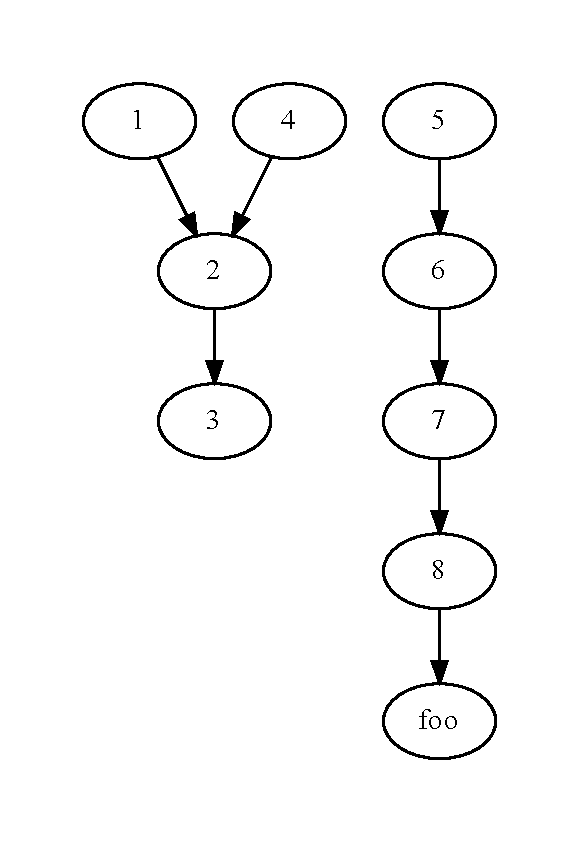
\includegraphics[scale=0.5]{cfg.pdf}
        \end{center}
        \caption{Initial CFG}
\label{fig:cfg0}
\end{figure}
Hypothetically circumscribing over the $\pred{successor}{\cdot, \cdot}$ predicate representing known transitions gives us a ``complete'' control flow graph to pass to a value analysis.
This circumscription assumed that $\forall{X}. \neg \pred{successor}{3, \var{X}}$.
However, the value analysis will quickly determine that \texttt{eax} may hold 4, and so finds $\pred{successor}{3, 4}$.
At this point, the informal version of this analysis reasons that since $\neg \pred{successor}{3, 4}$ contradicts itself, the next step is to assume $\pred{successor}{3, 4}$.\footnote{\
        It is actually possible to avoid reasoning from contradiction here: since VSA\cite{vsa} will only widen its value upper bound in response to new edges, and new edges are being discovered via these upper bounds, at a minimum those edges found in the current graph will be found in the true graph.
        However, VSA is still nonmonotonic, since the upper bounds it produces are invalidated (since they could become wider).
        Without modeling a property only present in composition, contradiction-based reasoning is unavoidable.
}

%   * Why is this call-CC?
One way to express such an ability would be to tie it to the law of excluded middle: $A \vee \neg A$.
However, an equivalent property $((A \imp \bot) \imp A) \imp A$ better captures the action of the evaluation procedure conceptually.
First, the evaluator guesses that $A$ cannot happen during the circumscription, i.e. $(A \imp \bot)$.
From that, it derives $A$.
As a result, outside the circumscribed world, we want $A$ to be visible as a fact.

% Bidirectional Proof Search
\section{Bidirectional Proof Search}
\label{sec:bidisearch}
In the background, I reviewed forwards (\S~\ref{sec:fchain}) and backwards (\S~\ref{sec:bchain}) chaining analyses.
Which to use is generally selected situationally, but I argue that for our use case, both are needed.
% * Forwards chaining = datalog
\subsection{Forwards Chaining}
Forwards chaining corresponds to the simpler ``do this when possible'' style of organization that program analysis authors are likely more familiar with.
%   * Want this to represent things which
%     * Almost always need to be done
It is good for representing things that will nearly always need to be done,
%     * Can be done efficiently
can be done efficiently,
%     * Have a reasonably bounded extent
and whose extent is reasonably bounded.
If the analysis does not usually need to be done, it will fire when it does not need to.
If it cannot be done efficiently, it will burn resources that may be needed elsewhere.
If its extent is not reasonably bounded, the analysis will pollute the database with a large morass of facts.

%   * Examples
There are several good examples of analyses which fit the forward chaining mold well.
%     * Parse
Parsing the binary container format will need to be done before nearly every other kind of analysis, is quite fast, and will produce facts bounded linearly in the size of the input binary.
%     * Lifting
Lifting of an address identified as executable will nearly always be needed to make any further queries about it, is a constant time operation per address, and produces a bounded data value.

%   * Good for preprocessing/directed auto-analysis
Overall, forwards chaining gives a good representation of what is normally viewed as preprocessing or auto-analysis.

% * Backwards chaining = prolog
\subsection{Backwards Chaining}
Backwards chaining corresponds to the ``do this when needed'' strategy of execution analogous to what occurs in user facing analysis tools or program property checker.
%   * Want this to represent things which
Backwards chaining is more appropriate for representing analyses which
%     * Rarely need to be done
are rarely needed,
%     * Are potentially expensive
are potentially expensive to run,
%     * Have an enormous or infinite extent
or have a large (or infinite) extent.

%   * Examples
While I expect most basic functionality to work well as forward-chaining analyses, some standard techniques simply do not fit well with it.
%     * Fuzz
Fuzzing is possibly one of the clearest cases.
A fuzzing run generates a vast amount of data, and can potentially generate an arbitrary amount by triggering with new random values.
These runs are also generally expensive.
%     * Solve this function for stack overflow with symex + smt
Another example of an analysis that fits better with backwards chaining is property checking via symbolic execution and SMT solving.
While the extent is small, it is potentially slow and has a wide variety of potential entry points/properties, very few of which are actually interesting.
% * Execution strategy
\subsection{Execution Strategy}
While my execution strategy is largely informed by my implementation strategy, it still reflects similar semantics to what is seen in the inspiration languages.
%   * Queries / rule firing acts as a transaction, multiple may be in flight
First, rule firings are treated as transactions, with conflicts being negotiated by the database.
This allows for a good deal of parallelism because with the exception of circumscription, no conflicting writes should occur to the database.
The one apparent downside of this is that analyses may potentially need to be rolled back (especially if they take longer to finish) if the database had a conflicting update via a circumscription.
However, had the same operations been performed in order, the run would still have been invalidated eventually.
In parallel, using transactions, Holmes will
\begin{itemize}
%   * Try to fire any legal forwards chaing rules until quiescence
\item Run any forwards chaining rules which have new body matches.
%   * If a query is received
\item If a query is recieved,
        \begin{enumerate}
%     * Output known matches
                \item Output known matches
                \item Add a goal root to the database for the given goal if not already present.
                \item Upon a request for more, give any new results present to the client
                \item Upon termination, decrement the goal root refcount or remove it if this is the only request.
        \end{enumerate}
\item Perform a tabling backwards search\footnote{\
                Strategy is to be decided, but may be anything from rule order to previous execution time, to a learning system.
        } for any root goals whose search has not been completed.
\end{itemize}

\section{Semantics}
To give a slightly more formal view of what I expect this system to do, I provide a derivability relation.
These rules are rough, but I hope they will help make my intentions more clear.

In these rules, the $\Gamma$ context is a bag context that is allowed weakening only when $\Delta$ is empty.
$\Gamma$ represents monotonically true facts and rules, a context of immutable truth.
$\Delta$ is an ordered context.
$\Delta$ is used to contain assumptions made thus far, with the rightmost assumption being the most recent.
$P^\tau$ and similar expressions are used to represent a predicate which has $\tau$ used as a free variable.
$E[x/y]$ is used to represent the substitution of $y$ for $x$ in the expression $E$.
I use $\vec{x}$ throughout to act as a shorthand for $x_1 \ldots x_n$.
\newcommand{\ds}{\vdash}
\begin{gather*}
  \infer[id]{\Gamma, a : P; \Delta \ds a : P}{}\\
  \infer[xchg]{\Gamma_0, x, \Gamma_1, y, \Gamma_2; \Delta \ds z}{\Gamma_0, y, \Gamma_1, x, \Gamma_2; \Delta \ds z}\\
  \infer[weaken]{\Gamma, x; \cdot \ds y}{\Gamma; \cdot \ds y}\\
  \infer[rule]{\Gamma, r : \forall \tau_0 \ldots \tau_n. ((P_1^{\vec{\tau}} \ldots P_m^{\vec{\tau}}) \rightarrow Q^{\vec{\tau}}); \Delta \ds r(\vec{\sigma}, \vec{p}) : Q^{\vec{\tau}}[\vec{\tau}/\vec{\sigma}]}{\Gamma; \Delta \ds p_1 : P_1^{\vec{\tau}}[\vec{\tau}/\vec{\sigma}] & \cdots & \Gamma; \Delta \ds p_m : P_m^{\vec{\tau}}[\vec{\tau}/\vec{\sigma}]}\\
  \infer[monagg]{\Gamma; \Delta \ds \{\vec{a}\} : P^\tau[\tau/(\leq \rho)]}{\Gamma; \Delta \ds a_1 : P^\tau[\tau/\sigma_1] & \cdots & \Gamma; \Delta \ds a_n : P^\tau[\tau/\sigma_n] & \bigvee \vec{\sigma} \leq \rho}\\
  \infer[hypcirc]{\Gamma; \Delta\vdash [\vec{a}] : (|\tau. P^\tau| = \vec{\sigma}) \Rightarrow P^\tau[\tau/\vee = \rho]}{\Gamma; \Delta \ds a_1 : P^\tau[\tau/\sigma_1] & \cdots & \Gamma; \Delta \ds a_n : P^\tau[\tau/\sigma_n] & \bigvee \vec{\sigma} = \rho}\\
  \infer[assume]{\Gamma; \Delta,  |\tau. P^\tau| = \vec{\sigma} \ds e : Q}{\Gamma; \Delta \ds e: (|\tau. P^\tau| = \vec{\sigma}) \Rightarrow Q & \forall a : P^\tau[\tau/\rho] \in \Gamma. \rho \in \vec{\sigma}}\\
  \infer[unassume]{\Gamma; \Delta \ds e : (|\tau. P^\tau| = \vec{\sigma}) \Rightarrow Q}{\Gamma; \Delta, (\vec{\sigma}, \tau, P^\tau) \ds e : Q}\\
  \infer[callcc]{\Gamma; \Delta, |\tau. P^\tau| = \vec{\sigma'} \ds callcc(e, e') : P^\tau[\tau/\vee = \rho']}{
    \begin{array}{ccc}
      \vec{\sigma'} = \vec{\sigma} + \gamma & \rho' = \rho \vee \gamma & \gamma \not \in \vec{\sigma} \\
      \Gamma; \Delta, |\tau. P^\tau| = \vec{\sigma} \ds e : P^\tau[\tau/\gamma] & & \Gamma; \Delta, |\tau.P^\tau|=\vec{\sigma} \ds e' : P^\tau[\tau/\vee = \rho]
  \end{array}}
\end{gather*}
The first three rules (id, xchg, weaken) establish the basic framework in which we are working (as per the context explanations above).

The ``rule'' rule expresses the basic way in which rules can be applied to facts.
This rule is similar to parametrically polymorphic function application.
The primary difference is that $Q$'s expression may contain an invocation of an external function, and so until the selection of the type paramter vector $\vec{\tau}$, you can't actually know what type the proof term has.

The ``monagg'' rule describes monotonic aggregation.
I use the notation $\leq \rho$ to represent a value for which we know that the meet of all values is at least less than $\rho$.
In actual use, you'd likely see e.g., $P(1, \leq \{2, 3\})$ or something similar.
The rule itself essentially says that if you have a proof for $P^\tau$ with each of a nubmer of different options, and their meet is less than some bound, then their set comprises a proof of $P^\tau$ with $\tau$ monotonically aggregated to $\rho$.

The ``hypcirc'' rule describes the procedure for hypothetical circumscription.
The construct $|\tau.P^\tau| = \vec{\sigma}$ is meant to represent that the total extent of assignments to $\tau$ for which $P^\tau$ may be derived is $\vec{\sigma}$.
This can be thought of (roughly, this is informal) as $\not \exists \gamma. (\gamma \not \in \vec{\sigma}) \wedge \Gamma; \Delta \vdash e : P^\tau[\tau/\gamma])$
What hypcirc allows is the use of the meet of a set of possible assignments to $\tau$ as an approximation of the true meet of all assignments, with the assumption added to the type.

The rules ``assume'' and ``unassume'' help guide search.
The ``assume'' rule is for limited movement of an assumption from the type of a proof term into the context.
The ``unassume'' rule inverts assume, but is unlimited, since we are not limited in what assumptions may occur on the right of the turnstile.
``assume'' in particular is very much not in its final form.
Currently, it only allows movement from the left hand side of a $\Rightarrow$ to the $\Delta$ context if there is not an identity-based proof of its assumption being wrong.
In a more complete version of this rule, the premises would contain a stronger notion of the concept of having failed, potentially temporarily, to produce contradictory proofs despite trying.
In this way, hypothetical circumscriptions which can be absorbed into the assumption context will be similar to stratified negation.
The primary difference between a limited assume and stratified negation will be that it is more permissive in what having tried hard enough to derive the fact is before it is allowed to assume it is false.

``callcc'' implements the assumption expansion in case of contradiction discussed previously (\S \ref{sec:callcc}).
If we can derive a contradiction to the most recent assumption, the $callcc$ constructor allows us to update the meet based on the knowledge of the flawed assumption.
It takes in a proof of a contradiction of the assumption, a predicate derived from the meet of that assumption, and updates it to contain the new information.

While these rules are rough, I hope they serve to give an idea of the intended derivability relationship.
\section{Implementation Strategy}
\label{sec:impl}
As I've begun the implementation of this system, I have already made several design decisions.

% * Lang = rust
%   * Safe
%   * Efficiently handles large data
%   * Threading story
For implementation of the logic engine itself, I have decided to use Rust\cite{rust}.
Rust is a safe, multithreaded language which provides C/C++ style direct control of allocation, copies, and other such processes.
This means that while I will not suffer as much overhead as more traditional safe languages, I will not be plagued by the issues I had with an initial C++ prototype.\footnote{\
        Combining C++ closures for asynchronous callbacks with multithreading brings up a number of surprising edge cases, none of which are checked for by the compiler.
        This was consuming too much development time, and I forecasted it would only get worse.
}

% * Database engine = postgres
To hold the data, I've selected Postgres.
%   * Transactions (multiple rules in flight)
%   * Joins (avoid writing a custom query compiler for match terms, just compile to joins)
Like most modern SQL systems, Postgres supports transactions and joins.
Transactions are important to allowing multiple rules in flight, as they provide clean synchronization.
Joins allow me to compile the match clauses of rules into SQL queries, substantially speeding up search in larger databases.\footnote{\
        An earlier naive in-memory prototype was actually much slower despite the faster access speed.
I made the decision to use a database layer when I realized the indexing code I was about to begin writing was roughly equivalent to the code in a standard SQL database.
}
%   * Efficient jsonb support for custom user data structures
Finally, Postgres is unique in providing efficiciently indexable, binary stored \texttt{JSON} objects through its \texttt{jsonb} extension.
While this will not be required initially, it will make allowing user defined datatypes, especially ASTs and similar structures, much easier later.

% * RPC system = Cap'n'proto
To bind analyses to the logic engine to allow their functions to be called, I either need to link them in, load shared libraries, or use an RPC system.
I ruled out linking in to allow for interpreted languages and avoid recompilation.
Plugins (shared library building) were ruled out because they are tricky for potential developers to build, and would again rule out interpreted languages.
As a result, \sysname\ requires an RPC system.
To fill this gap, I selected Cap'n Proto\cite{capnproto}, a system from a creator of Google's Protobuf\cite{protobuf}.
The primary reasons for selecting Cap'n'proto were multilanguage support, capability support, efficiency, and embeddability of dynamic structures.
Supporting many languages will ease the writing of analyses for \sysname.
Capability support both allows analyses to easily follow a ``registration'' pattern (sending an object to the server constructed with the relevant callbacks), and allows for lazy reading of large values such as traces or process image dumps.
Efficiency of the encoding is important to allow for the transfer of larger objects involved in binary analysis, such as traces\footnote{\
Traces are regularly many gigabytes in size.
}
The ability to embed dynamic structured binary data through reflection will make it easier to support analysis-defined types later on in the effort.

% * See impl in progress at my github
You can view the implementation in progress on GitHub.\footnote{\url{http://github.com/maurer/holmes}}

\newcommand{\hu}{\mathbb{U}}
\newcommand{\hb}{\mathbb{B}}
\newcommand{\cons}[1]{C(#1)}
\newcommand{\decides}{\triangleleft}
% NFI = no force inconsistent
%\newcommand{\nfi}[2]{{#1} \triangleleft^? {#2}}
\newcommand{\world}[1]{W({#1})}
\newcommand{\stepass}{\leadsto}
\newcommand{\circset}{K}
\newcommand{\aggset}{A}
\newcommand{\decirc}[2]{D(#1, #2)}
\newcommand{\viol}[2]{V(#1, #2)}
\newcommand{\trule}[1]{\textsl{#1}}

\chapter{Formal Holmes}
\label{chap:formal}
Holmes differs from base datalog in callbacks (analogous to external predicates), aggregates, circumscription, and call/cc.
External predicates already have a well understood semantics, and we will model callbacks as interpreted functions by extension of our Herbrand universe during instantiation (\S \ref{formal:sec:callbacks}).
Aggregates in the presence of interpreted functions can be replaced by a syntactic tranformation, other than for purposes of circumscription.
Adding call/cc forces a solution to exist when it otherwise would not, adding a restricted set of solutions which violate the minimality constraint of stable set semantics when no stable set exists.

We will first go over the negation model embedded at base datalog to demonstrate how it works more clearly (\S~\ref{formal:sec:negation}).
Then, we will show how to construct the Herbrand universe for a program with callbacks, aggregates, and circumscription (\S~\ref{formal:sec:herbrand}).
Finally, I will give semantics for the Herbrand instantiation of a Holmes program which interprets circumscription as infinite negation, and call/cc as the failure of one of those negated terms (\S~\ref{formal:sec:semantics}).
%TODO add any proofs to intro
\section{Negation}
\label{formal:sec:negation}
\subsection{Other forms of Negation}
The first primary distinction to draw in negation is ``strong negation'' vs ``negation-as-failure'', or NaF.
Strong negation describes having knowledge that something is not the case, whereas NaF describes knowing that we will never have proof that something is the case.
This difference is more formally defined by Gelfond and Lifshitz~\cite{strongneg}, where strong negation is referred to as classical negation.
In this work we will focus on negation-as-failure.

One way of interpreting negation is ``stable-set'' semantics~\cite{stablemodel}.
In stable-set semantics, to check a whether a proposed model is a stable set, we first take the reduct of the logic program under the proposed model.
To do this, we remove all negated body clauses which are not present in the proposed model (and so are satisfied), and then remove all rules which still have negated clauses in them (which were not satisfied).
If the model is the minimal model of this reduct (this new reduced program), then it is a stable set, or stable model of the program.
This interpretation admits an arbitrary number of potential stable models, including none.

Another approach is known as ``well-founded negation''~\cite{wellfounded}.
This approach constructs what it calls ``unfounded sets'', which are sets of values which, relative to a given partial interpretation, can never be proven.
It then augments the partial interpretation with the negation of the unfounded set, and constructs a new minimal model, treating negated clauses as only true if explicitly present in the new partial interpretation.
This procedure is run unto fixpoint, and produces exactly one well-founded partial model, which will be a subset of all stable models~\cite{wellfounded}.

In our case, stable-set semantics leaves something to be desired due to the potential for no model, and the well-founded approach may return partial solutions.
\subsection{Negation in Holmes}
Traditional datalog consists only of a head clause, implied by a series of body clauses.
To this, we allow clauses to be optionally negated.
In the original input program, the head clause may not be negated.

As we have no function symbols or interpreted functions, we define a Herbrand universe $\hu$ which is simply the set of constants in the program.
$\hb$ is the set of every predicate instantiated at every combination of values in $\hu$.

We instantiate the program into the Herbrand universe, making a version of each rule with every variable instantiated at every member of $\hu$.
This eliminates pattern matching and reduces all rules ot a set of rules of the form
\[
	p \leftarrow \bigwedge q_i \wedge \bigwedge \neg r_j
\]
where $p, q_i, r_i \in \hb$.
While there will be no rules of this form in the initial translation of the program, we also allow rules of the form
\[
	\neg p \leftarrow
\]
which simply asserts $\neg p$.
We will use $N$ to describe a possibly negated term, e.g. it has form $p$ or $\neg p$ where $p \in \hb$.

For a program $\Pi$ which consists of a set of such rules,
\[
	\infer[\textrm{m.p.}]{\Pi \models N_0}{N_0 \leftarrow \bigwedge_{i \in I} N_i \in \Pi & \forall i \in I. \Pi \models N_i}
\]

We will define an interpretation of negation in such programs via a Kripke frame.
We say a program $\Pi$ is consistent if it does not model both truth and falsehood for a single fact.
\[
	\infer[\textrm{consistent}]{\cons{\Pi}}{\forall p \in \hb(\Pi). \Pi \models p \imp \Pi \not \models \neg p}
\]
We say a program $\Pi$ decides a fact if it models it as either true or false.
\[
	\infer[\textrm{decide-true}]{\Pi \decides p}{\Pi \models p}
	\quad
	\infer[\textrm{decide-false}]{\Pi \decides p}{\Pi \models \neg p}
\]
We give a base case for a program $\Pi$ being a world if it is consistent and it decides all facts.
\[
	\infer[\textrm{world-base}]{W(\Pi)}{C(\Pi) & \forall p \in \hb(\Pi). \Pi \decides p}
\]
We say a program $\Pi$ does not force the inconsistency of a fact if either it decides that fact, or adding one of its truth or negation results in a world.
\[
	\infer[\textrm{nfi-decided}]{\nfi{\Pi}{p}}{\Pi \decides p}
	\quad
	\infer[\textrm{nfi-true}]{\nfi{\Pi}{p}}{\world{\Pi \cup (p \leftarrow)}}
	\quad
	\infer[\textrm{nfi-false}]{\nfi{\Pi}{p}}{\world{\Pi \cup (\neg p \leftarrow)}}
\]
Finally, a program is a world in our Kripke frame if it does not force the inconsistency of any fact, nor is it already inconsistent.
\[
	\infer[\textrm{world}]{\world{\Pi}}{\cons{\Pi} & \forall p \in \hb(\Pi). \nfi{\Pi}{p}}
\]

The world-base rule is equivalent to the world rule with only the nfi-decided rule available for not forcing inconsistency.
It is included to show more clearly the inductive construction of whether a program is a world.

We define a relation between worlds $\stepass$ describing assumptions that may be made from a given program.
\[
	\infer[\textrm{assume-false}]{\Pi \stepass \Pi \cup (\neg p \leftarrow)}{p \in \hb(\Pi) & \Pi \not \decides p & \world{\Pi \cup (\neg p \leftarrow)}}
\]
\[
	\infer[\textrm{assume-true}]{\Pi \stepass \Pi \cup (p \leftarrow)}{p \in \hb(\Pi) & \Pi \not \decides p & \world{\Pi \cup (p \leftarrow)} & \neg \world{\Pi \cup (\neg p \leftarrow)}}
\]

We complete the Kripke frame by defining the accessibility as transitive closure over $\stepass$.
\[
	\infer[\textrm{refl}]{\Pi \leq \Pi}{}
	\quad
	\infer[\textrm{assume}]{\Pi_0 \leq \Pi_2}{\Pi_0 \leq \Pi_1 & \Pi_1 \stepass \Pi_2}
\]

We consider a formula $F$ true for an input program $\Pi$ if $\Pi \models \dia \boks \dia F$ under this frame.
Here, $\dia$ means ``possibly'', and $\boks$ means ``necessarily'', so this condition says that it is possibly necessarily the case that this formula is possible.
We can visualize this on a directed graph with worlds as nodes and and the single-step form of our accessibility relation ($\stepass$) as an edge.
This condition means that if we start from $\Pi$, our input program, we can find a connected program $\Pi'$, so that no matter what path we take forwards from there, there will always be a path to a world where the formula $F$ holds.
Conceptually, this means that there exists an allowed choice of assumptions so that $F$ becomes a conclusion we will always eventually reach.

assume-false represents normal circumscription.
Adding the assume-true is what differentiates our negation model.
This rule only allows the assumption of truth if assuming false would either make the world inconsistent immediately, or make it impossible to provide a consistent assignment to the remainder of the facts given that assumption.
By adding assume-true, we allow a consistent solution in the presence of negation in some cases it would not otherwise be possible.
By restricting it to those cases where assuming falsehood would result in a forced inconsistency in any complete model, we still rule out trivial solutions like setting everything true, but in a looser way than the minimal model over the reduct.
It is looser because it allows for models which are not minimal over the reduct, as when assume-true is used, it adds a true proposition which has no derivation from the rules, and so would not be present in any minimal model.
As assume-true is only allowed in cases where assume-false would lead to no solution, it still prohibits the trivial solution (all predicates are in the model).

In Holmes, circumscription corresponds to a potentially-infinite variety of assume-false in which every version of a specific aggregate greater than the proposed circumscription is negated.
call/cc corresponds to assume-true, but is a bit more complex, since it needs to discern at least one specific assumption from the infinite negation arm which is untenable.

\section{Herbrandization}
\label{formal:sec:herbrand}
First, we define the Herbrand universe and base.
Then, we describe how to instantiate a Holmes program at this universe.

\subsection{Herbrand universe}
\label{formal:sec:callbacks}
Instead of function symbols which produce new values, as in a traditional construction, we have interpreted functions and and lattice joins.
This is different from the normal construction because interpreted functions both interpreted functions and lattice meets may produce values which are equal to existing values.
To address the equality issue, we assume that our construction is supplied with implementations of the callbacks and join operations as the real program would, and actually execute them on input values rather than creating symbolic expansions.

Define $U_0$ to be those constants present in the program, combined with varieties tupled up to the maximum arity of the provided functions.
Consider joins as equivalent to callbacks which just happen to return only one argument.
Let $F$ be the set of functions, modified to take tuples for multiple arguments, and to return their results ``flattened'', e.g. if a callback would return $a = 1, b = 2$ and $a = 3, b = 4$, its representative in $F$ returns $\{1, 2, 3, 4\}$.
Since both meets and callbacks are typed, if an input would be outside their domain, they return $\emptyset$.

Given $U_i$, construct $U_{i + 1}$ by
\[
	U_{i + 1} = \bigcup_{x \in U_i, f \in F} f(x)
\]
We then combine these stages:
\[
	\hu = \lim_{j \rightarrow \infty} \bigcup_{0 \leq i < j} U_i
\]

The Herbrand base $\hb$ is constructed in the usual way, instantiating each predicate at every value of $\hu$.

\subsection{Program Instantiation}
For predicates which have aggregation, rewrite them as rules with interpreted functions.
If we have
\[
	P(\tau_0 \cdots \tau_m, \sigma_0\wedge j_0 \cdots \sigma_n \wedge j_n)
\]
then we create a new function
\[
	j(a_0 \cdots a_n, b_0 \cdots b_n) = \{c_0 = j_0(a_0, b_0) \cdots c_n = j_n(a_n, b_n)\}
\]
and add the rule
\[
	P(x_0 \cdots x_m, c_0 \cdots c_n) \leftarrow P(x_0 \cdots x_m, a_0 \cdots a_n), P(x_0 \cdots x_m, b_0 \cdots b_n) + j
\]
where $+ j$ as in the informal Holmes description means to attach the function $j$ to run after the match to generate a set of assignments to variables in the head clause not bound by the body.
For each aggregated predicate, introduce a circumscripted version of the predicate, $P_c$.
Perform simple replacement of all circumscripted matches to $P$ with matches against $P_c$.

Now, the program looks like normal datalog but with functions attached to some rules.
For every element of the Herbrand universe, instantiate the rule, run the function concretely on the variables bound in the body clause, and instantiate the head term.
This will result in a rules of the form
\[
	p \leftarrow \bigwedge q_i
\]
where $p, q_i \in \hb$.

\section{Semantics}
\label{formal:sec:semantics}
We begin by defining a few extra sets relative to the initial program which will be needed for interpretation.
Let $\circset(\Pi) \subseteq \hb(\Pi)$ be the set of circumscripted facts added, e.g. they were of the form $P_c(\cdot)$.

Let $\aggset(\Pi)$ be a set of tuples of an aggregated predicate and all of its non-aggregated inputs.
For example, for $P(x_0, \cdots x_n, y_0, \cdots y_m)$ and all $y$ are aggregated, $(P, x_0, \cdots x_n)$ for each possible value of $x_0$ through $x_n$ would be present in $\aggset(\Pi)$.
We will refer to members of $\aggset(\Pi)$ as ``aggregates''.

Let $\circset_a(\Pi)$ where $a \in \aggset(\Pi)$ be the set of circumscriptions which correspond to that aggregation specifically.
This is a partitioning of $\circset(\Pi)$.

Let $\decirc{\Pi}{c}$ where $c \in \circset(\Pi)$ be the non-circumscribed version of the fact, e.g. if $c$ corresponds to $P_c(x_0 \cdots x_n)$, then $\decirc{\Pi}{c} \in \hb$ corresponds to $P(x_0 \cdots x_n)$.

Let $\viol{\Pi}{c} \subseteq \hb$ be those predicates which are \emph{directly} negated by the circumscription.
This contains all of those values belonging to the same aggregate which are not less than or equal to the circumscription.


Much of this is similar to the simple negation semantics, but I restate it here for clarity.

\[
	\infer[\textrm{consistent}]{\cons{\Pi}}{\forall c \in \circset(\Pi). \Pi \models c \imp ((\forall p \in \viol{\Pi}{c}. \Pi \not \models p) \wedge \Pi \models \decirc{\Pi}{c})}
\]
Like previously, consistency here requires that a none of the negations assumed by a circumscription also be present in the model in a non-negated form.
Specifically, the rule says that for all circumscripted facts in the universe, if they are in the model of the program, then none of the conditions which would violate the circumscription hold, and the aggregated fact corresponding to the circumscripted fact holds.
Additionally, the circumscription must be supported: the aggregate must have reached the point on the lattice that the circumscription asserts will be the exact value.

Rather than deciding individual facts as we did previously, we now decide aggregates.
\[
	\infer[\textrm{bounded}]{\Pi \decides a}{c \in \circset_a(\Pi) & \Pi \models c}
	\quad
	\infer[\textrm{no-base}]{\Pi \decides a}{\forall c \in \circset_a(\Pi). \Pi \not \models \decirc{\Pi}{c}}
\]
The bounded case indicates that we have circumscribed this aggregate, and so have decided it.
The no-base case indicates that this aggregate is totally unpopulated by the program.
Since our lattices are not gauranteed to be bounded, no circumscription can be made.
As we cannot circumscribe over it, we are considered to decide the aggregate.
Specifically, the program has decided on the negation of all values which could make up the aggregate.

This time, since our $\stepass$ is more complex, our world predicate and $\stepass$ are defined mutually recursively.
We also index $\stepass$ with the aggregate that it either circumscribes or extends.

\[
	\infer[\textrm{world}]{\forall a \in \aggset(\Pi). \Pi \decides a \vee \exists \Pi'. \Pi \stepass_a \Pi'}{\world{\Pi}}
\]
A program is a world if for every aggregate, it either decides it, or there is a one-step accessibility to one where it is circumscribed or extended ($\stepass_a$).

\[
	\infer[\textrm{circ}]{\Pi \stepass_a \Pi \cup c}{\Pi \not \decides a & c \in \circset_a(\Pi) & W(\Pi \cup c)}
\]
If $a$ isn't decided yet, and circumscribing it closed would not cause any inconsistency, we may do it.

For call/cc, let $\Pi_c$ be $\Pi$, but modified so that $\viol{\Pi}{c} = \emptyset$ and $c$ is unioned in.
In other words, $\Pi_c$ is $\Pi \cup c$, but will ignore inconsistencies which are based on the addition of $c$.
\[\small
	\infer[\textrm{call/cc}]{\Pi \stepass_a \Pi \cup p}{\Pi \not \decides a & \world{\Pi_c} & \not \exists c'. \Pi \stepass_a \Pi' \cup c' & \not \exists p' \in \viol{\Pi}{c}. \Pi \models p' & p \in \viol{\Pi}{c} & \Pi_c \models \dia \boks \dia p}
\]
This rule says that if we cannot construct $\stepass_a$ using the circ rule, but $\Pi_c$ would extend the aggregate $a$ with new information, then we can extend $a$ with the new information even though the proposed circumscription would not result in a world.
We define $\leq$ based on $\stepass$ exactly as before.

Finally, we hold a formula to be true for a Holmes program if the program $\Pi$ it is translated into can access a world where all accessible worlds can access a world where the formula is true. More succinctly, $\Pi \models \dia \boks \dia F$.

\newcommand{\aliasname}{{\sc Marduk}}
\newcommand{\subheading}[1]{\textbf{#1.}}

\chapter{Alias Analysis}
\label{sec:alias}
In order to show that Holmes can be used in practice, we implement a concrete system with it.
We chose to focus on the problem of use-after-free, as it is a little-explored area for static binary analysis.
We used Holmes here to link together control flow analysis, alias analysis, string recovery, and general function loading in order to build a working use-after-free engine.

% Use after free bugs are common
There were 238 use-after-free (UaF) vulnerability disclosures (CWE-416) issued in 2017 alone, with 36.2\% given a critical security
rating.
% From cvedetails.com, mitre doesn't seem to issue CVE/CWE associations.
Use-after-free bugs happen when a pointer has been freed and the memory pointed to subsequently written to or read from.
Use-after-free bugs can lead to DoS, control flow hijack, and information leaks.

Despite the number of CVEs, few tools exist that can automatically and statically detect such bugs in off-the-shelf \emph{binary} code.
However, there are tools for finding such bugs in \emph{source} code.
Requiring source code limits the applicability of these techniques to developers with full source access.

In this chapter, we focus on the question
``Can we use \sysname\ to bridge the gap between analysis for UaF bugs in source code versus compiled code?''
In particular, previous work has been unable to apply source code techniques to compiled code.
Can we adapt such techniques to be effective even without source?

At a high level, UaF bugs require reasoning about memory allocation and memory aliasing.
Source code techniques are more plentiful due to the rich and mature research area of alias, points-to, and similar schemes for reasoning about memory over the lifetime of a program.
In comparison, at the binary level the primary approach for reasoning about memory is Value Set Analysis~\cite{vsa}, which is less mature and has several limitations in practice such as inability to reason about all arithmetic operations (e.g., bit-shifts and division) and the fact it may not terminate without ad-hoc widening in the presence of loops.
For example, GUEB~\cite{gueb} was proposed to detect UaF bugs using VSA, but is handicapped by disallowing cyclic paths to allow rapid termination of VSA.

We present a new binary-level static analysis approach for detecting UaF bugs in executable programs.
One of the main technical challenges we address is showing how to adapt source-code memory alias analysis to compiled code, where previous work has instead created all-new binary-only approaches to alias
analysis like VSA.
We experiment with two classes of analysis: flow insensitive alias analysis via a Steensgaard-type~\cite{steensgaard-alias} algorithm, and  flow-sensitive alias analysis using a data flow approach adapted from Andersen~\cite{andersen} style analysis with added rules to handle binary-specific details such as calling conventions and computed addresses.
We also add context-sensitivity by allowing the analysis to reason about the call-stack discipline followed by executable code, and a type of field sensitivity appropriate for direct pointer arithmetic without type information.
To the best of our knowledge, very little work has been done in applying the literature in source alias analysis to compiled code, and no previous work has shown how to then use such techniques to find UaF bugs statically in compiled code.

We have built a tool called \aliasname\ that uses \sysname\ to drive the different levels and co-dependencies in binary analysis, alias analysis, and UaF detection.
Taking this approach allows us to have an end-to-end reasoning chain from input binary to why this particular candidate use-after-free could not be disproven with a given sensitivity.

We evaluated \aliasname\ over 7 real CVEs and the Juliet test suite released by IARPA for purposes of verifying our detection capabilities and measuring false positives in the face of bugs.
Additionally, we measured false positive rates against a background of expected-good binaries (we assume no true positives): a random sampling from the \texttt{\$PATH} of a default Ubuntu installation.

\aliasname\ is available at \url{https://github.com/maurer/marduk}.

\section{Analysis Design}
\label{alias:sec:system}
First, our system transforms the input binary into structured
semantics we can work with throughout the rest of the process.
Second, we perform alias analysis over the structured representation.
This allows us to know all the pointers which may point to freed
memory after each free.  Finally, we look for reads and writes through
potentially freed pointers to create our list of candidate
use-after-frees.

\subsection{Alias Analysis}
Alias analysis consists of computing the possible ways to access different variables.
If dereferencing two expressions may access the same variable, they are said to alias.

Our machine-level alias analysis involves three main design choices that must be addressed:
\begin{enumerate}
\item Selecting variables.
  Alias analysis is performed over program variables, but unlike C, the assembly from a binary does not contain variable information.
\item Selecting sensitivity.
  We can return points-to information parameterized on different pieces of context.
  Common examples of parameters are flow sensitivity (program location), context sensitivity (call stack), field sensitivity (offsets within memory regions), and object sensitivity (possible construction sites for a ``this'' pointer).
  In this work, we examine, flow, context, field, and recency~\cite{vsa}, how to implement them on compiled code, and their effects on precision and performance.
\item Solving for points-to relationships.
  The generation of the aliasing information is undertaken differently for flow-insensitive vs flow-sensitive varieties of alias analysis.
  The flow-insensitive variety uses a constraint satisfaction technique and simultaneous solving via Steensgaard~\cite{steensgaard-alias}.
  Flow-sensitive varieties use the inter-procedural dataflow described in \S \ref{sec:interproc}.
\end{enumerate}

\begin{figure}
	\centering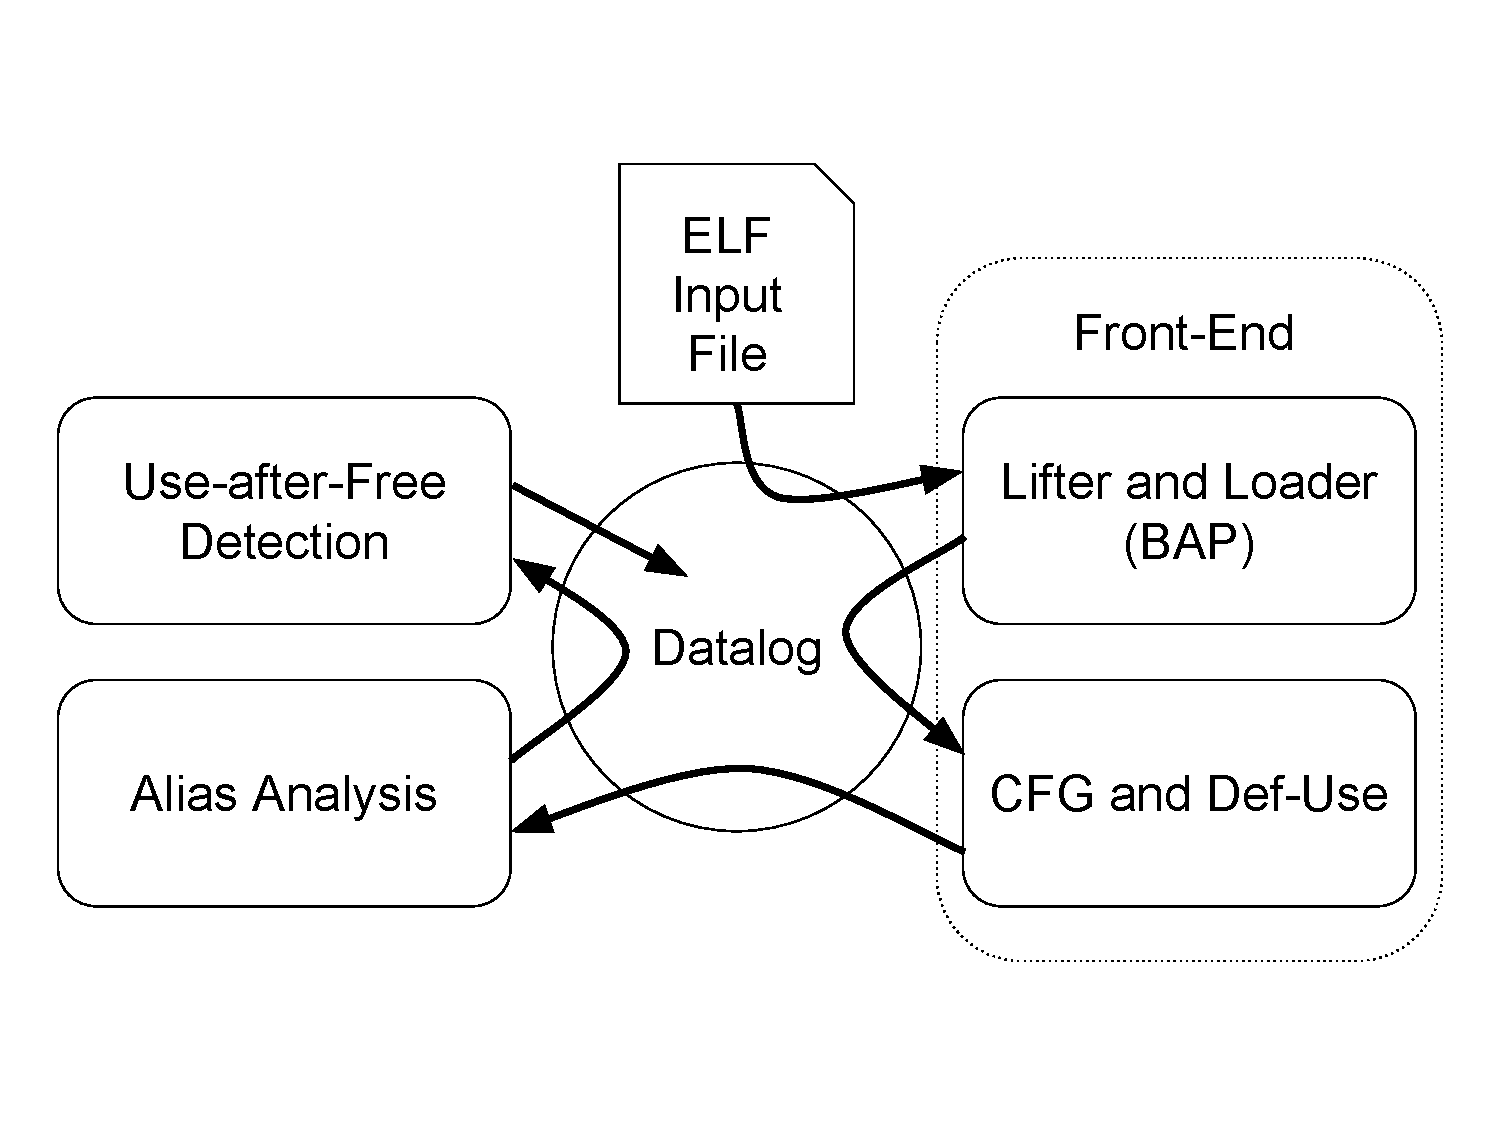
\includegraphics[scale=0.3]{alias/system.pdf}
	\caption{System Diagram}
	\label{fig:system}
\end{figure}

\subsection{Front-End}
Before we can apply our analysis, we first need to transform the raw
bytes of the input file into a form similar to the AST\footnote{Abstract Syntax Tree} received after
parsing.  Techniques in this section are not novel, and are described
for completeness to understand our overall system.

The front end:
\begin{itemize}
  \item Parses the executable file container, e.g., ELF on Linux
  \item Finds potential function entry points
%TODO if I do a codependence trial, forward reference here
  \item Builds a control flow graph
  \item Provides an intermediate language with the semantics for every reachable instruction
  \item Builds a call graph and call-site information
\end{itemize}

We use the BAP~\cite{bap} framework to provide ELF parsing, entry point identification, and instruction semantics.

\subheading{Variables}
In our approach, we use 3 kinds of variables:
\begin{itemize}
	\item Stack slots, parameterized by which function they are in. Written \texttt{sp+off@func}
	\item Registers
	\item Dynamic Allocations, parameterized by the location at which they are allocated. Written \texttt{dyn@loc}
\end{itemize}
We use an abstract location in these parameterizations.
In the context-insensitive case it is simply the address of the instruction, and in the context-sensitive case it is the pair of the address with the return stack.

Our choice of dynamic allocation variables defines our heap model.
We assume that two memory regions may only alias if they were allocated at the same program point.
This assumption matches reality unless a pointer has been released back to the allocator via free, but then used afterwards (a use-after-free bug).
This may violate the assumption because a write to or read from the now freed pointer may alias with newly returned memory.
As a result, this heap model is correct at least until the first use-after-free in an execution.
As we are not performing a value analysis, we also assume all accesses are in-bounds.
Essentially, if a use-after-free is the \emph{first} memory violation to occur, we will locate it.

\subheading{Calculating Update Summaries}
In order to avoid analyzing the full complexity of IL instructions within alias analysis, we first transform them to contain only the relevant dataflow information.
Our update summaries are then a description of the action of an IL instruction on the points-to relationship, where \texttt{a} and \texttt{b} are variables as defined above:

\begin{itemize}
\item \texttt{a = b}
\item \texttt{a = *b}
\item \texttt{a = \&b}
\item \texttt{*a = b}
\item \texttt{*a = *b}
\item \texttt{*a = \&b}
\end{itemize}

A list of these is generated for each instruction and associated with
the location of the instruction.  At allocation sites we emit the
summary \texttt{a = \&dyn@loc}, meaning that the variable \texttt{a}
(usually \texttt{RAX}) takes on the address of the allocation region
corresponding to that location.  % In our example~\ref{lst:example-asm}
% we would emit \texttt{RAX = \&dyn@0} for the instruction on line 4
% (location 0).  In the context-insensitive case, this gives us an
% abstraction parameterized only on the address of the malloc; values
% from one allocation site are assumed to never alias with those from
% another.  In the context-sensitive cases, this summary additionally
% parameterizes the abstraction by the return stack at allocation time.

\subsection{Insensitive Analysis}
In the flow-insensitive case, we modify the summaries before use to adapt our variable selection to better fit the problem.
Specifically, we annotate registers with definition sites, similar to what might be found in SSA form.

We compute the possible definition sites of each register on the right side of a summary, and clone the summary for every possible definition.
If the left side of a summary contains a register, we parameterize it with the location it came from.
We do this because a single register may hold many different logical variables at different points of time.
The register location parameterization allows us to avoid every definition of a register being potentially readable from every other site in the program.
Without our approach, the resulting alias sets would be too imprecise to be useful as a register's alias set (e.g., \texttt{RAX}) would include information about all variables ever assigned to \texttt{RAX} by register allocation.
Notably, this would include every call to \texttt{malloc}.
This parameterization adds a little bit of flow sensitivity even in otherwise insensitive analysis.

We then aggregate all update summaries from the program and solve them by equality via Steensgaard's algorithm.
Steensgaard runs  in almost linear time~\cite{steensgaard-alias} making it possible to compute over nearly any binary, though is less precise than flow-sensitive analysis, described below.
We use insensitive analysis as a baseline to help quantify the additional precision derived by adding additional sensitivity.




\subsection{Adding Flow Sensitivity}
Our flow sensitive analysis is structured as a dataflow problem.  At each assembly instruction, we use a transfer
function based on Andersen's~\cite{andersen} inclusion-style analysis.
We use the inter-procedural dataflow adaptation described next (\S\ref{sec:interproc}).
The same rules and functions are used to handle both context-sensitive
and context-insensitive analysis, as the Location's stack context is
considered optional.

A dataflow analysis is defined by a transfer function which calculates how a statement should update the dataflow facts
(alias sets in our case),
a set of control flow edges to walk from a set of starting points,
and a meet function with specifies how to merge information sets at control flow graph confluence points.
We describe these below.

By default, alias analysis calculates alias sets even when a variable is dead.
We run a pass before alias analysis to determine which variables are live.
While calculating alias analysis, we use this information to remove dead points-to information to improve performance and precision.
Performance is increased because we do not waste time and space updating and tracking points-to
sets we know will never be used.
Precision is increased because if no pointers to a given allocation exist any longer, we know any new pointer to that allocation points to copy of that region which does not need the information from the old copy.

\subheading{Transfer Function}
The actual processing of the update summaries based on summaries is calculated via the transfer function.
We follow Andersen as shown in Listing \ref{lst:process}:
\begin{itemize}
\item Definitions of variables are performed destructively.
\item Writes through variables are applied to each value they may point to.
\item Right hand sides go through 0, 1, or 2 levels of dereference for \texttt{\&b}, \texttt{b}, and \texttt{*b} respectively to generate the set to update with
\end{itemize}

\begin{figure}
	\centering
	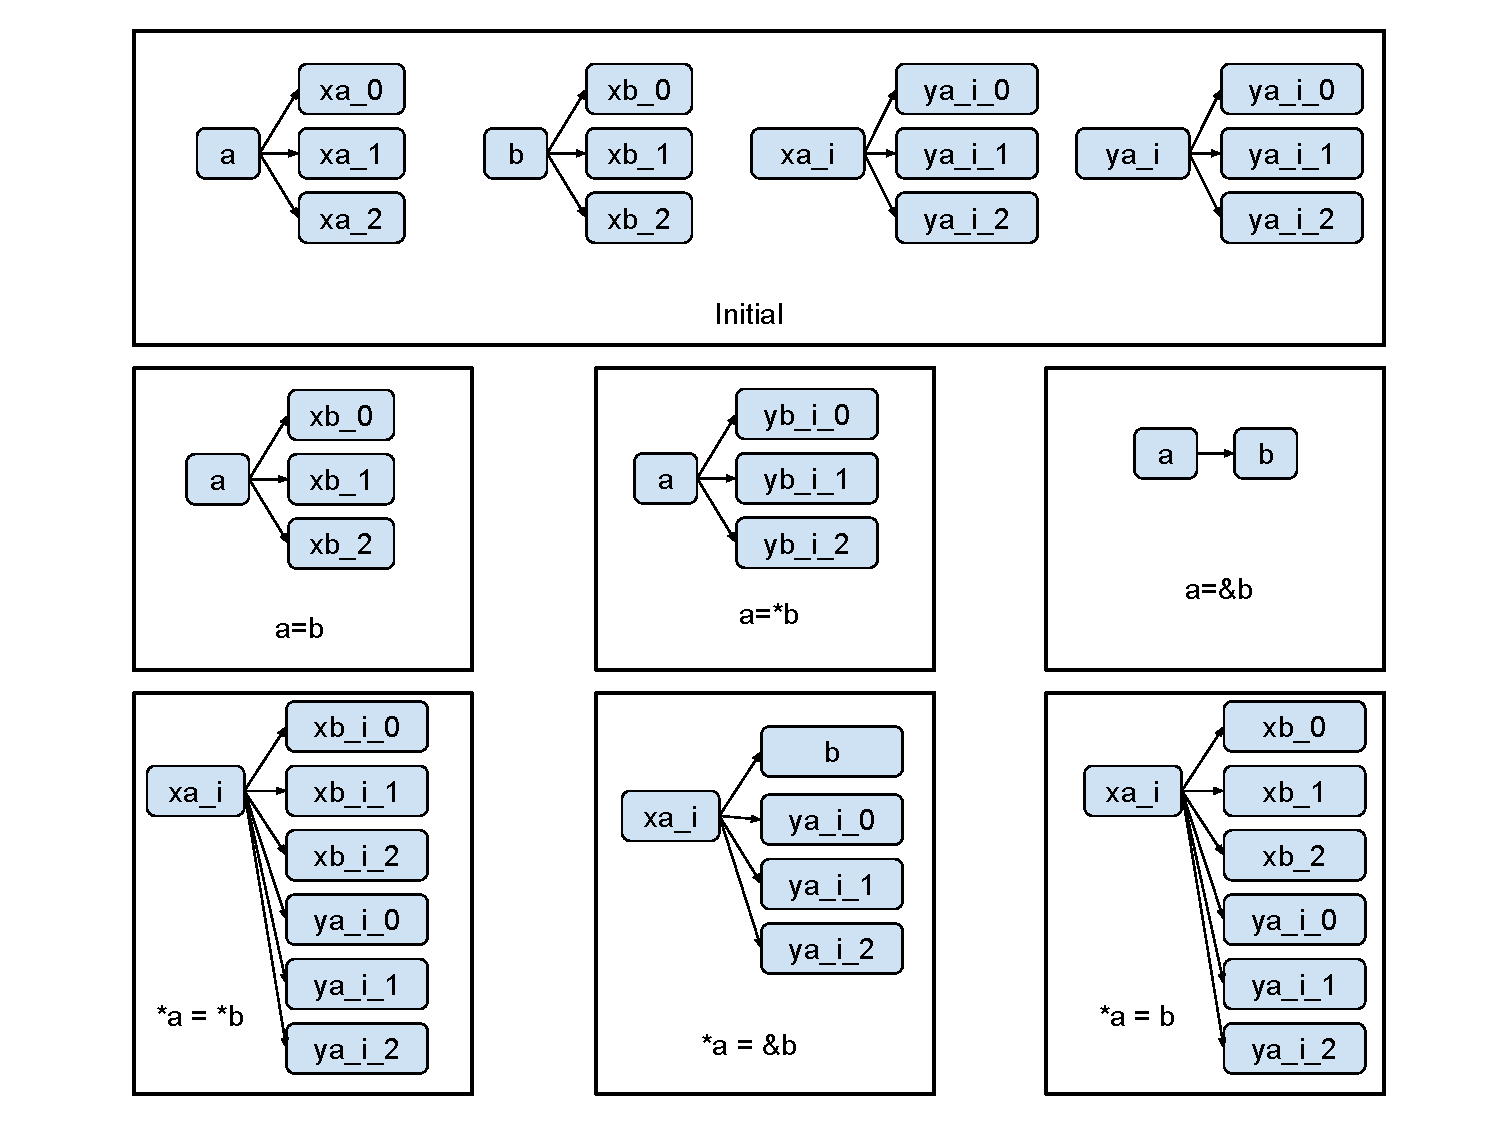
\includegraphics[scale=0.35]{alias/pts-update.pdf}
	\caption{Points-to Updates}
	\label{fig:pts-update}
\end{figure}

Figure~\ref{fig:pts-update} shows the transfer function rules for each
statement type.
%This is illustrated in Figure \ref{fig:pts-update}.
The ``Initial'' section shows a sample initial configuration a points-to relation might have.
Each other region is labeled by a statement, and shows what would change about the points-to relation.
Each time an ``i'' is used on the left, assume that portion is present 3 times, with i ranging from 0 to 2.

For updates to stack slots or registers, we can perform a ``destructive'' update.
This is demonstrated in the \texttt{a =} examples in Figure \ref{fig:pts-update}.
This means that since we know the new value
is the only value the variable could have, we can \emph{replace} the
points-to set.  In the case of pointer write though, we cannot do
this, because our analysis is not field sensitive.

In a field sensitive analysis, this destructive update logic would be
extended to writes through pointers with a points-to size of one,
allowing for more destructive updates and increasing the precision of
our analysis.
We will explain and add field sensitivity shortly in section \ref{sec:field}, but until then, pointer updates need to remain non-destructive.

After we complete the updates to the points-to structure, we remove
all variables which are no longer live according to the previously computed information.
These variables will never be used, so tracking them is imprecise and expensive.

Finally, we perform a mark-and-sweep garbage collection of the tracked pointers, using stack slots, registers, and anything that was pointed to at the entrance of the function as roots.
This last caveat is necessary so that if an argument to a function is written to, and then never used again, the parent will still see the update even though the callee no longer knows how to reference the region.
This allows us to \emph{forget} about allocations which are no longer accessible.

\paragraph{Dataflow}
\begin{lstlisting}[float=*t, caption={Flow Sensitive Pointer Analysis Rules}, label=lst:flowrules]
flow_in(Location, PointsTo^pt_union)
flow_out(Location, PointsTo)

flow_init: flow_in(loc, {}) <- malloc_call {loc}

flow_step: flow_in(dst, pts) <-
  succ {src, dst, is_call: false, is_ret: false} & flow_out(src, pts)

flow_xfer: flow_out(loc, pts2) <-
  flow_in(loc, pts) & updates(loc, us) & kill(loc, ks) & live {loc, live}
  & flow::xfer(pts, us, ks, pts2)
\end{lstlisting}
\begin{lstlisting}[float=t, caption={Process Update}, label=lst:process]
match update {
  (*\bfseries *a = \&b*) =>
    for a_target in pts[a] {
      pts_out.add(a_target, b)
    }
   (*\bfseries a = \&b*) =>
     pts_out.replace(a, {b})
   (*\bfseries a =  b*) =>
     pts_out.replace(a, pts[b])
   (*\bfseries a = *b*) =>
     pts_out.replace(pts[pts[b]])
  (*\bfseries *a =  b*) =>
    for a_target in pts[a] {
      pts_out.add(a_target, pts[b])
    }
  (*\bfseries *a = *b*) =>
    for a_target in pts[a] {
      pts_out.add(a_target,
                  pts[pts[b]])
    }
}
\end{lstlisting}

The overall flow rules we use are shown in  Listing \ref{lst:flowrules}.
Andersen-style analysis formulates updates as inclusion constraints, rather than equality constraints like Steensgaard.
In the initial declaration of predicates, \texttt{flow\_in} is declared to aggregate via set union on each points-to set.
Since each \texttt{flow\_in} value at a location produces a unique \texttt{flow\_out} value, aggregation is not necessary on that predicate.
We create an empty input map at every allocation site, because allocation is the only action which will add information to an empty points-to relation.
\texttt{flow\_step} propagates points-to relations along normal succession edges.
Finally, \texttt{flow\_xfer} performs the meat of the operation, absorbing the update summaries into the current context by applying the transfer function.

\subsection{Inter-procedural Dataflow}
\label{sec:interproc}
Our approach to inter-procedural dataflow follows the example of Reps~\cite{interproc-dataflow} with some modifications.
While many optimizations described there are inapplicable to our domain, the general structure still applies.
At the site of a call, an inter-procedural edge is added from the call site to the target function.
Following this edge elides stack slots which are not currently pointed to.
This is a departure from Reps in that their restricted domain, all local variables were not passed through.
An intra-procedural edge is added which skips over the call, applying effects (see \S \ref{sec:effects}) and clobbering variables not preserved by the function.
Finally, at each return site, an inter-procedural edge which forgets the stack slots local to that function if not pointed to is added.
We do not report an error even if a local stack slot is pointed to, as this is a legal possibility in the case of a recursive call which passes one of its stack variables by reference.
Again, we depart from Reps here by keeping around what would normally be local variables if they are pointed to.

\texttt{flow\_call} and \texttt{flow\_ret} apply when functions are entered and exited to cut down on unnecessary information being propagated around, applying the restrictions for our inter-procedural edges, as described earlier.

\texttt{flow\_call\_over} propagates information at a call site \emph{over} a function call, skipping it but removing definitions for variables known to be overwritten by the function.
This corresponds to the special intra-procedural edge added to our dataflow when processing a call.
This rule also enables analysis through functions which were not provided, albeit with the assumption that the function was effectively a no-op.

\begin{lstlisting}[float=*t, caption={Inter-procedural Rules}, label=lst:interrules]
flow_call: flow_in(dst, pts2) <-
  succ {src, dst, is_call: true} & flow_out(src, pts)
  & flow::call(pts, dst, pts2)
flow_ret: flow_in(dst, pts2) <-
  succ {src, dst, is_ret: true} & flow_out(src, pts) & func {base, contains: dst}
  & flow::ret(pts, base, pts2)
flow_call_over: flow_in(dst, pts2) <-
  call_over {src, func, dst} & flow_out(src, pts)
  & flow::over(pts, pts2)
\end{lstlisting}

\begin{lstlisting}[language=C, float=t, caption={Example (C)}, label=lst:example-c]
char* g() {
	return malloc(1);
}
void f() {
	char* x = malloc(1);
	*x = 'a'; // Safe
	char* g_a = g();
	*g_a = 'a'; // Safe
	char* g_b = g();
	*g_b = 'a'; // Safe
	free(x);
	free(g_a);
	*x = 'b'; // UaF
	*g_b = 'b'; // Safe, but needs context
}
\end{lstlisting}

\subsection{Inter-procedural Flow-Sensitive Example}
In this section, we provide an example of the context- and flow-
sensitive analysis on a simple example shown in
Listing~\ref{lst:example-c}. To provide clarity on how updating alias
sets work, this example does not show data-flow merges, which is a set
union operation as previously described.

Listing \ref{lst:example-c} contains one real use-after-free bug.  We
also show one location that is safe, but without context-sensitivity
an additional false positive will be raised. Without
context-sensitivity, both the allocations for \texttt{g\_a} and
\texttt{g\_b} get merged, making the analysis believe they are aliased
when they are not.

\lstdefinestyle{hilight-asm}{
    language={[x86masm]Assembler},
    moredelim=[is][\color{green}]{|+}{|},
    moredelim=[is][\color{blue}]{|!}{|},
    moredelim=[is][]{|~}{|},
    basicstyle=\footnotesize 
}

\lstinputlisting[style=hilight-asm,
caption={Annotated Flow-Insensitive Analysis},
label=lst:example-asm]{alias/example-annotated.asm}

The corresponding assembly, annotated with comments on the location of
the UaF and alias sets, is shown in Listing~\ref{lst:example-asm}.
Portions of the alias set hilighted in green are new bindings.
Portions in blue are bindings which have been destructively updated.
In the example, the variables are:
\begin{itemize}
	\item The stack slots of f (g has none): sp+24@f, sp+16@f, sp+8@f
	\item All used registers (other than the stack): RDI, RAX
	\item Allocations split on sensitivity, using the form dyn@addr\{stack\}
          \begin{itemize}
          \item Context-insensitive: dyn@5 and dyn@13
          \item Context-sensitive: dyn@5\{19\}, dyn@5\{25\}, dyn@13\{\}
          \end{itemize}
\end{itemize}

The alias sets are annotated as comments. For example, right before
the free on line 35, the alias set is:

\begin{figure}[h!]
\texttt{\{ RAX -> dyn@0; sp+24@f -> dyn@1;
    sp+16@f -> dyn@0; sp+8@f -> dyn@0;
    RDI -> dyn@0 \}}
\end{figure}

This shows that \texttt{RDI} is pointing to the memory location \texttt{dyn@1}, the allocation site for \texttt{x} in the source code.
Right after the \texttt{free} on line 35, the alias set changes to show \texttt{dyn@1} is now free.
The UAF detector would say any pointer that resolves to \texttt{dyn@1} is therefore a use-after-free bug, which happens on
line 53.

If we had been context-sensitive, the points-to relation at 59, the false positive, would instead be
\begin{figure}[h!]
\texttt{\{ RAX -> dyn@5\{25\}; sp+24@f -> dyn@13\{\};
    sp+16@f -> dyn@5\{19\}; sp+8@f -> dyn@5\{25\};
    RDI -> dyn@5\{19\}; dyn@13\{\} -> free@35;
    dyn@5\{19\} -> free@43 \}}
\end{figure}

The key difference here is that \texttt{RAX} points to \texttt{dyn@5\{25\}} rather than just \texttt{dyn@5}, so we can distinguish it from the freed allocation.
This allows context sensitivity to weed out more false positives.




\subsection{Adding Context Sensitivity}
Context-sensitivity requires we only change our \texttt{Location}
values to contain information about the stack.
We add an empty stack to entry points to initialize the new stack-enhanced CFG.
Called functions must copy their control flow graphs to separate versions for every stack at which they are being called.
When generating the target of a call function, we now add the current instruction's fallthrough to the stack as a return address.
If the return address is already on the stack, we truncate the stack so that it is the topmost.

Unfortunately, with an unbounded stack, of our real-world samples (\S \ref{alias:sec:eval:real}), this approach exhausts available resources (128G RAM) for all but \texttt{gnome-nettool}.
To remedy this, we use a $k$-stack approach combined with the stack truncation above.
If a call is made from a location parameterized by a stack, it is first checked to see if the call site is present.
If so, it is truncated as before.
Otherwise, it is pushed onto the stack, and if the stack is longer than $k$, the oldest entry is removed.
In the case of our example, a stack size of 1 would be sufficient, and we'd see the allocations \texttt{dyn@0\{10\}}, \texttt{dyn@0\{11\}}, and \texttt{dyn@1\{\}}.

\subsection{Adding Field Sensitivity}
\label{sec:field}
%TODO add arith and widening
Up until now, we've been treating each memory region like a single homogeneous bag:
Anything written into it ever can be read out again on any subsequent read.
This reduces precision.

In traditional alias analysis, field sensitivity can be done by simply treating each variable with a struct type as though it were several - one for each field.
Unfortunately, in the binary case, things are slightly messier for two reasons: overlapping fields, and variable offset writes.
Since this is only a pointer analysis, not a general value analysis, we only consider fields with size equal to the pointer size.

Previously, we used a simple set to denote what a variable might point to.
We now replace this with a ``field map''.
We will use the word ``reference'' to describe the pair of a variable and an offset.
The offset may be a fixed value, or a special value indicating a computed offset.

A field map has two components: a set of references for unknown offsets, and a set of references for some subset of possible fixed offsets.
If a fixed offset read is performed, we return the offset's set if defined, otherwise the unknown set.
If a computed offset read is performed, we return the union of every set (both unknown and fixed) present in the map.

We split update rules into cases for a single pointer write (so we know which memory cell was updated precisely) and for multiple.

\subheading{Single Pointer}
If a fixed offset write is performed on a variable, we destructively update the set corresponding to that offset.
If a computed offset write is performed, we extend both the unknown set, and every tracked offset to contain the new reference.
If an overlapping field is written to, the field it overlaps is emptied.

\subheading{Multiple Pointers}
If a fixed offset write is performed on a variable, extend the set corresponding to that offset.
If a computed offset write is performed, we extend both the unknown set, and every tracked offset to contain the new reference.
If an overlapping field is written to, nothing happens.

This structure is conservative so long as we accept the assumption that pointers are not constructed piece-wise.
Specifically, if pointers are constructed over the course of multiple writes, we will not know about them.
This limitation was present in the previous, field insensitive formulation, but becomes more obvious in the description of the field sensitive extension.
This practice is extremely uncommon (outside bulk copy functions like \texttt{memcpy}, which may be summarized), so we accept this limitation to limit the need to reason about the exact possible values of a computed offset.

Unfortunately, this formulation gives the alias analyzer slightly too much power.
Specifically, it can now count.
Despite the fact that we did not model actually performing arithmetic, a pointer being incremented in a loop will look like repeatedly examining relative offsets of a struct.
To deal with this, we add a widening operator\footnote{
	A widening operator is an addition to a dataflow analysis which provides termination by moving further on the lattice than is strictly necessary under certain conditions.
}which, if the same variable points to a fixed limit or more offsets in a region, will replace it with pointing to an unknown offset to that region.
This reclaims termination.

\subsection{Recent Allocation Domain}
\label{sec:effects}
Using the site or site and size of an allocation to define the allocation domain is fairly common.
However, this can have poor behavior around loops:

\begin{lstlisting}
char* x;
while(1) {
site_0:
	x = malloc(1);
	*x = 'a';
	free(x);
}
\end{lstlisting}

If running a dataflow computation to fixpoint, on the second
iteration, the allocation for \texttt{site\_0} will appear already
freed.  The usual response to this type of imprecision is to unroll
loops a fixed number of times.  However, our tool is intended to be
complete (assuming a complete control flow graph, provided functions,
etc.) so we want to avoid fixed unrollings.

To this end, we extend our allocation domain with a ``recent'' bit, similar to the MRAB vs NMRAB abstraction~\cite{vsa}, though for different purposes.
Relative to a concrete trace, the address most recently given by an allocation at a given site belongs to the set where ``recent'' is true.
All other addresses issued by that site belong to the set where ``recent'' is false.
In our static form, a value belongs to the recent set for an allocation site if there exists some trace for which it was the last allocated from that site.
It belongs to the non-recent set if there exists some trace for which it was not most recently allocated.
Note that once in static form, the recent set may have more than one member, and may even intersect with the non-recent set.

This extension is a departure from the normal Andersen alias analysis.
It is only for precision, not correctness.
It can essentially be viewed as 1 bit path-sensitivity, where path-sensitivity would be parameterizing on entire sequences of instructions which could be taken to reach the current point.

To implement this in our static alias analysis, we construct summaries for each function of allocations and possible allocations.
When processing the edge which skips the function which is meant to propagate variables not accessible to it, we update the points-to relation using information from this summary to keep recency information accurate.
We do this by modifying the behavior of \texttt{flow\_call\_over} to update the caller points-to to represent what may have happened in the callee.

We define an ``effect'' to be a set of definite allocation sites and a set of possible allocation sites that occur when a call is made.
To apply an effect to a points-to set:
For every definite allocation site, make the recent bit false.
For every possible allocation site, duplicate any recent references to have both recent and non-recent values.
Listing~\ref{lst:recent} shows this change.

%To this end, we amend the rules as in Listing \ref{lst:recent}
\begin{lstlisting}[float=*t, caption={Rules for Recent Domain}, label=lst:recent]
flow_call_over: flow_in(dst, pts2) <-
  call_over {src, func, dst} &
  flow_out(src, pts) &
  (*\bfseries func\_effect \{func, effect\} \&*)
  (*\bfseries flow::over\_effect(pts, effect, pts2)*)

local_effect {base: Location, local: Location, effect: Effect}
func_effect {func: Location, effect: Effect^effect_merge}

effect_init: local_effect {base, local: base, effect: no_op} <- func {base}
effect_ret: local_ret: func_effect(base, effect) <-
  succ {src: local, is_ret: true} &
  local_effect {base, local, effect}
effect_xfer: local_effect {base, local: local2, effect} <-
  succ {src: local, dst: local2, is_call: false, is_ret: false} &
  local_effect {base, local, effect}
effect_call: local_effect {base, local: local2, effect: effect2} <-
  call_over {src: local, func: remote, dst: local2} &
  func_effect {func: remote, effect: effect_call} &
  local_effect {base, local, effect} &
  effect::sequence_effect(effect, effect_call, effect2)
effect_malloc: local_effect {base, local: local2, effect: effect2} <-
  succ_over {src: local, dst: local2} &
  local_effect {base, local, effect} &
  malloc_call {loc: local} &
  effect::malloc(effect, local, effect2)
\end{lstlisting}

There are four new functions here.
\texttt{effect\_merge} will merge two local effects at a confluence point.
It does this by intersecting their definite allocations, and migrating all other allocations to possible allocations.
\texttt{flow::over\_effect} will apply the effect to the points-to set in addition to its earlier responsibilities.
\texttt{effect::sequence\_effect} will update the currently processed effect with the called function's effect by unioning together both possible and definite effects, then removing those possible effects which are also definite.
\texttt{effect::malloc} just adds the current site as a definite allocation to the effect.

The result is that these effect summaries allow greater precision over allocation sites, similar to what is achieved through loop unrolling, but without sacrificing fix-point semantics.

In our example earlier, this would give rise to three allocations - \texttt{dyn@0}, \texttt{dyn@1+old}, and \texttt{dyn@1}.
This would suppress the false positive by distinguishing between the two invocations of \texttt{g}.
However, were a third added, it would not be able to distinguish between the first two invocations of \texttt{g}.

\subsection{Use-after-Free}
With alias relationship in hand, we must determine which reads and writes in the program are use-after-free candidates.
For the flow and flow \& context analyses, we can augment the alias analysis itself to track most of this information for us.
When a free occurs, we generate a special form of the \texttt{*a = \&b} summary, with \texttt{a} as the pointer being freed, and \texttt{b} as a special value representing things freed at that location.
This is as presented in Listing \ref{lst:uafflow}.
\texttt{read\_vars} generates pointer access information from actual assembly instructions, and \texttt{use\_vars} imports it from summaries which can do things like determine argument count to \texttt{printf}.

\begin{lstlisting}[label=lst:uafflow, caption={Tracking Frees with Flow Sensitivity}]
read_vars: deref_var(v, loc) <-
  lift {loc, bil} &
  func {base, contains: loc} &
  uaf::reads_vars(bil, v)
use_vars: deref_var(v, loc) <-
  uses(r, loc) &
  uaf::use_vars(r, v)

free_summary: summary(loc, s) <-
  free_call{loc, args} &
  uaf::free_summary(args, s)
uaf_flow: uaf_flow(v, loc, loc2) <-
  deref_var(v, loc2) &
  flow_in(loc2, pts) &
  flow::is_freed(pts, v, loc)
\end{lstlisting}

However, this approach only works with alias information that is at least flow sensitive.
Without flow sensitivity, any pointer which was ever freed will appear freed everywhere in the program, even before it was freed.
As a result, the false positive rate would be absurd, and such a detector would be more a heap-access detector than a use after free detector.
To help it along and make the difference in false positive rates more about the precision of the alias information rather than the ability to track state changes, we add a few extra conditions to report a use after free without flow sensitivity by essentially doing flow sensitive tracking of the freed-property only.

\begin{lstlisting}[label=lst:uafins, caption={Tracking Frees Insensitively}]
base_freed: freed_base(v, loc) <-
  free_call {loc, args} &
  uaf::free_args(args, v)
all_freed: freed_var(v2, loc) <-
  freed_base(v, loc) &
  steens_point(v, vs) &
  uaf::expand_vars(vs, v2)

path_init: path_exists(loc, loc) <-
  freed_base(_, loc)
path_step: path_exists(loc, loc3) <-
  path_exists(loc, loc2) &
  succ_any {src: loc2, dst: loc3}

uaf: uaf(v, loc, loc2) <- freed_var(v, loc) & path_exists(loc, loc2) & deref_var(v, loc2)
\end{lstlisting}

The implementation of this modification is shown in Listing \ref{lst:uafins}.
In the first stanza, we mark the variable freed by the free call and everything it aliases with as potentially freed at that location.
In the next, we find those parts of the program reachable from the free site.
We then finalize the results by saying that if a path exists from a freed variable to a dereference of that same variable, then there is a use after free candidate.
While this is certainly imperfect, going much further would begin to graft flow sensitive information into the otherwise insensitive analysis.

\section{Implementation}
\label{alias:sec:impl}
Our implementation consists of 3k lines of Rust and 234 lines of datalog.
Each additional sensitivity (field, context, flow, recency) is implemented by adding an additional datlaog file.
The switches to determine which sensitivities actually run operate by adding initial facts to the database to suppress unwanted rule triggers.
As a result of this design, other than field sensitivity (which requires significant logic in both the constraint generator and points-to set structures), these additional sensitivites can be compiled out safely by simply removing the rules in question (and their associated bound functions).

\subsection{Limitations}
Our system is conservative in almost all cases, but there are a few notable exceptions.
If the provided file is linked against files which are not provided, their functions will be assumed to effectively be no-ops.
If in reality, these functions free memory or write to the heap, this may cause missed vulnerabilities.
The system uses the BAP control flow graph and any indirect jump resolution and the analysis assumes they go nowhere; we do no additional resolution beyond \texttt{ret} calls.
%This may result in an incomplete control flow graph, which in turn can lead to %missed bugs.
Control flow recovery is a general problem in binary analysis and not specific to our approach.
Essentially, if a prerequisite step gives our algorithm incomplete information, it will produce an incomplete result.
This was sufficient for the programs analyzed, which are written largely in C, but some resolution would be required to achieve good quality result on C++ programs which use vtables or programs which use a callback architecture (and so rely heavily on function pointers).

We assume the transfer of a pointer from one place to another will take place in a single assembly instruction - we do not model ``the first 3 bytes of a pointer to x'' for example.
Finally, we assume that a traditional stack discipline is being followed for purposes of points-to minimization in the sensitive cases.
If it is not, aliases from stack calculations pointing above or below your own stack frame may be missed.

\section{Evaluation}
\label{alias:sec:eval}
Our evaluation has 3 major components.
\begin{itemize}
\item Juliet - How do we perform on a labeled (true positives, false positives, false negatives) data set?
\item Real World Bugs - Can we detect real bugs? 
\item Ubuntu \texttt{\$PATH} - How often do we alarm on real bug-free code?
\end{itemize}

We evaluate over the Juliet test set both for comparability with other work~\cite{tac, juliet-eval-static-source} and to act as a baseline for our detection power and false positive rates.
It helps answer the question ``In the absences of confounding factors from the real world, how well does this work?''.
We also evaluate over real use-after-free bugs pulled from MITRE's CVE database.
Evaluating on these verifies that real world code, while potentially confounding, does not stop our technique from functioning altogether.
It also provides a measurement of the false positive rate in the presence of true positives.
Finally, we evaluate over a variety of believed-good binaries.
The intent behind this evaluation is to get a better idea of false positive rates and analysis costs for average programs believed to be non-buggy.

\subsection{Juliet}
IARPA released the Juliet test suite~\cite{juliet} as a way of providing standardized examples of CWEs.
By building only those corresponding to use-after-free, we get a high density test suite.

All three sensitivities find all intended bugs in Juliet.
Insensitive analysis generates 39834 false positives, reducing to 0 with flow sensitivity.
Run time was 19m30s for the flow sensitive version, and 30m4s for insensitive.
However, the insensitive variety generates its alias information as of 3m23s.
The system spent the remainder of the time generating reachability information.

Unfortunately, while Juliet serves as a good test for true positives, it does not do much to elicit false positives from our system, which is why both our performance and others' look too-good-to-be-true here.
Within the negative tests, there is little in the way of things that checkers are traditionally weak against (data structures, recursion, loops, etc.).
For this reason, it is important to evaluate ourselves on real world code as well.

\subsection{Live CVEs}
\label{alias:sec:eval:real}
Our system successfully detects 7 real bugs across 6 programs.
All sensitivities of the checker detected all bugs.
We assume that all potential use after frees which do not match the known bugs in each of these programs are false positives.

\begin{figure*}
\begin{center}
\begin{tabular}{|c|c||c|c|c|c|}
\hline
Program & Sensitivity & Run time & Memory & False Positives & Binary Size\\
\hline \hline
\multirow{3}{*}{gnome-nettool} & Insensitive & 38s & 1G & 1851 & \multirow{3}{*}{156k}\\
	& Flow & 30s & 1G & 0 &\\
	& Flow + Ctx & 2m34s & 2G & 0 &\\
	\hline
\multirow{3}{*}{goaccess} & Insensitive & 4m35s & 15G & 387459 & \multirow{3}{*}{635k}\\
	& Flow & 16m14s & 10G & 112420 &\\
	& Flow + Ctx & 43m34s & 34G & 87 &\\
	\hline
\multirow{3}{*}{libarchive} & Insensitive & 1m23s & 3G & 4917 & \multirow{3}{*}{366k}\\
	& Flow & 34s & 1G & 852 &\\
	& Flow + Ctx & 22m12s & 44G & 7 &\\
	\hline
\multirow{3}{*}{shadowsocks-libev} & Insensitive & 2m12s & 5G & 130760 & \multirow{3}{*}{631k}\\
	& Flow & 3hr46m21s & 62G & 22357 &\\
	& Flow + Ctx & 3hr53m26s & 72G & 115 &\\
	\hline
\multirow{3}{*}{mdadm} & Insensitive & 16m45s & 31G & 1056570 & \multirow{3}{*}{768k}\\
	& Flow & 2hr24m13s & 42G & 270683 &\\
	& Flow + Ctx & 12hr10m43s & 111G & 14566 &\\
	\hline
\multirow{3}{*}{isisd} & Insensitive & 3m46s & 8G & 58241 & \multirow{3}{*}{451k}\\
	& Flow & 18m49s & 9G & 11776 &\\
	& Flow + Ctx & 22m32s & 25G & 513 &\\
	\hline
\end{tabular}
\end{center}
\caption{Real CVE Performance}
\label{fig:cveperf}
\end{figure*}

\begin{figure*}
	\begin{center}
	\begin{tabular}{|c||c|c|c||c|c|c||c|c|}
		\hline
		Sensitivity & \multicolumn{3}{c||}{Run time} & \multicolumn{3}{c||}{Memory} & \multicolumn{2}{c|}{Alarms} \\
		\hline
		& Avg & Median & Stdev & Avg & Median & Stdev  &Avg & Imp\\
		\hline\hline
		Insensitive  & 2m26.1s & 58.4s & 3m38.1s & 241.7M & 34.1M & 1.9G & 73.1 &\\ \hline
		Flow & 2m14.2s & 54.7s & 3m19.6s & 236.8M & 34.1M & 1.9G & 0.5 & 93.1\% \\ \hline
		Flow and Ctx  & 2m22.1s & 55.6s & 3m54.9s & 349.2M & 34.0M & 2.3G & 0.2 & 43.5\% \\ \hline
	\end{tabular}
	\end{center}
	\caption{Ubuntu \texttt{/usr/bin} Performance}
	\label{fig:ubperf}
\end{figure*}

Note that while the insensitive analysis completes quickly and cheaply for every binary, the false positive rates are so high that the output would be difficult to use.
Flow sensitivity reduces false positives significantly.
Manual analysis reveals that most remaining false positives are either due to data structure usage (which decreases the precision of the alias analysis), confused allocation sites from wrapped malloc constructors, and infeasible paths.
Context sensitivity gives additional improvements by helping to differentiate between instances of calling wrapped mallocs (e.g. \texttt{new\_foo()} to allocate and initialize a \texttt{foo}).


Performance for insensitive and flow-sensitive analyses appears similar in large part because the generation of a global program reachability graph for each \texttt{free} is costly.
If the analysis is instead timed in phases, the alias-analysis-only portion for the insensitive system takes seconds, while it takes the bulk of the non-CFG-recovery time in a flow-sensitive analysis.

For the known-vulnerable set, flow sensitivity reduced the false positive set by an average of 90\%, and context sensitivity reduced it by an additional 84.1\%.
The false positive reduction for the addition of flow sensitivity is immense, and the increase in time and space needed for the alias analysis was manageable for programs in our known-vulnerable set, the largest of which was 768kb.
Adding context sensitivity further increased the time and space cost, but still yielded a major increase in precision.

\subsubsection{GUEB}
The author of the GUEB~\cite{gueb} tool made his tool open source\footnote{
	\url{https://github.com/montyly/gueb}
}, allowing us to compare against it.
We connected IDA, BinNavi, and GUEB and ran the system over the same bugs we evaluated against.
As a caveat, we could not feed them the same binaries our tool consumed - their tool's stack only accepts 32-bit, so we recompiled the same vulnerable programs in 32-bit mode.

Figure~\ref{fig:guebperf} shows the performance.
The crashes derive from unhandled cases in the input, and not fundamental to their methods.
The undetected bugs occur due to their choice to not follow back edges (either as recursion or loops) when computing their VSA.
This is an understandable choice, since VSA can become slow and be difficult to force convergence for when cycles are present in the input, but in this case it caused their analysis to miss bugs.
Likely due to this forwards-only approach, GUEB terminated rather quickly on all inputs.

In Listing~\ref{lst:isisd-gueb}, we can see one of the real vulnerabilities the lack of a fixpoint fails to detect.
The loop knows that \texttt{adj} is allocated and non-null on entry, so the first time through the loop is always fine.
However, some paths through the loop free \texttt{adj}, and go around the loop again.
At this point, a use-after-free can occur.
If back edges are not followed, the analysis cannot detect this.

\begin{figure}
\begin{center}
\begin{tabular}{|c||c|c|}
\hline
Program & False Positives & Bug Found? \\
\hline \hline
	gnome-nettool & 2 & Yes\\
	goaccess & crash & crash\\
	libarchive & 222 & Yes\\
	shadowsocks-libev & crash & crash\\
	mdadm & crash & crash\\
	isisd & 596 & No\\
\hline
\end{tabular}
\end{center}
\caption{GUEB Performance}
\label{fig:guebperf}
\end{figure}

\begin{lstlisting}[language=C, float=t, caption={\texttt{isisd} Vulnerability}, label=lst:isisd-gueb]
// ... (adj is allocated and constructed here)
for (level = IS_LEVEL_1; level <= IS_LEVEL_2; level++) {
	// ...
	else if (new_state == ISIS_ADJ_DOWN) {
		// ...
		isis_delete_adj(adj);
	}
}
// ...
\end{lstlisting}


\subsection{Ubuntu Path Sample}
Now that we know that our program will alert us to real world vulnerabilities, we also want to know how it will behave in the case where no expected vulnerabilities are present.
To this end, we ran our program across \texttt{/usr/bin} on a default Ubuntu Xenial installation, as shown in Figure~\ref{fig:ubperf}.

Adding flow sensitivity provided an average reduction in bug candidates of 93.1\% in those situations where the insensitive code found at least one candidate.
Then adding context sensitivity ($k$ = 1) reduced it by an additional 43.5\%, in those situations where the flow sensitive analysis had a bug candidate, and the context sensitive analysis terminated.

Manual auditing of the reported bugs did not reveal any true bugs, but did show that a common pattern amongst false positives was functions for whom one path freed and replaced a pointer, and the other did neither, and they rejoined.
A more aggressive analysis for dead variables could remedy this by pruning them to allow the freed region to leave the points-to relationship before the paths rejoined.

The system emitted a maximum of 22 reports on individual binaries (and this worst case had most of them clustered in the same code area).
This was few enough reports to enable practical manual auditing by a single individual.
Unfortunately, none of these reports corresponded to real bugs upon examination.
This does not guarantee these programs are bug free - while we have a conservative analysis, that is dependent on seeing the entire control flow graph.
In this case this condition is not met.
Some C++ programs which use vtables are present in this path - calls to member functions there will appear as no-ops.
Function pointers are similarly considered to be no-ops.
Calls into libraries which were not analyzed with the binary are similarly absent.
Finally, some of these are GUI or threaded applications, which utilize a callback system we again do not handle control flow edges for.

\section{Related Work}
%Related Work
\section{Related Work}
\label{sec:related}
%  Starting blurb similar to backround blurb, surprised by this...
As this work stands at the confluence of compilation, instruction set architectures, static analysis, and type theory, there is a great deal of prior work that provided the foundation to create \bitr. There have been other attempts to perform binary type recovery. Type theorists have explored the relevant formal systems that enable us to appropriately describe the constraints imposed by the wide variety of instructions. Others have tried to build decompilers, each of which contains at least an attempt at type reconstruction.
%  Chunk related work into blobs and describe, reference to sections as you do it
\subsection{Types in Compiled Code}
In large part, previous work has considered dynamic approaches, which use execution traces to get information about concrete values. Another school of thought takes a more forensics-oriented approach, attacking the problem by looking for known data structures within a dump or trace. Finally, there is the school to which this work belongs, static type recovery, where the approach regenerates type information from a representation of the code, rather than from sample runs or matching known data structures.

\noindent {\bf Dynamic Type Description.}
Rewards~\cite{rewards} takes a dynamic, trace-oriented approach to the problem, taking execution traces and known system calls, and propagating types from system calls through the trace's reads and writes. The dynamic approach has the advantage that the analysis can know what values a memory location or register actually held at a given program point. Additionally, the dynamic approach does not have to solve the problem of indirect jumps, as when working with traces the next instruction is precisely computed. Finally, since Rewards had exact aliasing information via pointer values on each trace, flowing information from the system call barrier (their major outside source of types) is easier. While Rewards seems limited for types not present during the crossing of the system call barrier, its dynamic approach, and information from the crossing of the system call barrier could provide additional constraints to a system like \bitr\ to further improve accuracy. Howard~\cite{Slowinska2011} extends the work of Rewards by focusing on access patterns instead of simple propagation, and annotating variables from the original code, rather than locations on a dump.

\noindent {\bf Type Forensics.}
Another approach known as shape analysis~\cite{August, Haller2013a,White2013,Jung2009,Cozzie} uses dynamic traces to generate shape graphs, which they then analyze to make guesses at the types of memory locations. The systems generate the shape graph by first generating a trace, then matching the access pattern to the simplest possible graph of type structures. Some generate this trace from the compiled program, and some must annotate the program prior to compilation to achieve this trace. Once the system generates the shape graph, it compares the shape graph to multiple possibilities of what the data structure might be in attempt to classify it e.g. as a binary tree or linked list. One benefit of this technique is that when the system finds a match, more information on a name of the data structure may be available. However, if the program uses a data structure not expected by the system, some of these methods will fall short. For example, MemPick will report it to be a generic graph. It also suffers from the standard dynamic analysis issue of being unable to generate types for paths the test cases did not drive it down.

\noindent {\bf Static Type Recovery.}
Like TIE~\cite{tie}, we built \bitr\ on BAP~\cite{bap}, and also took the approach of trying to generate ranges of constraints. However, TIE performs much worse under our metric, which we feel more fully represents accuracy of more complicated types. TIE's metric is problematic for the reasons described in~\cite{sw}, but the proposed replacement metric is still dependent on a notion of distance. TIE is also slow, which hobbles its use as a large scale analysis tool. The use of DIVINE's methods was one of the bottlenecks, which we avoided in \bitr\ by recovering the type of everything that is addressable through the registers or a constant integer used along a dataflow that ended in a read or write. While the type system of TIE included structure types, TIE would rarely infer them, though its metric did not demonstrate this. Finally, if run on a static binary (e.g. without dynamic library hints), the amount TIE could infer itself was minimal.

SecondWrite~\cite{sw} instead takes the approach of lifting to a LLVM-based IR~\cite{llvm}, then using \texttt{mem2reg} to detect variables and LLVM pointer analysis to compute the types. Their reconstruction is simpler and faster than TIE's, but the approach has issues: \texttt{mem2reg} is a nice shortcut, but has the problem that \texttt{mem2reg} will not promote anything which has a use other than a load or store~\cite{llvm}. As a result, if on-stack references are in use, those stack slots will not be properly promoted to variables. Additionally, dependence on pointer analysis leaves them without a way to detect recursive types within their framework, and makes nested structures unlikely to work.

Another work focusing primarily on structure recovery~\cite{comprecon} approached the problem from the angle of figuring out what idioms compilers used to address arrays and structs, and then tried to reconstruct structs and arrays. However, by the authors' own admission, this approach cannot handle nested structs. Additionally, their dependence on assumptions about how the compiler will act and how the source language must work cause the output to be of limited use for understanding properties of code which was not necessarily built by the compilers or language expected.

\subsection{Type Theory}
Some of the inspiration for this form of type characterization \S\ref{sec:typesys} came from intersection typing~\cite{Jim1995,Shao1993}. Though we did not end up using intersection types for inferrability purposes (even the decidability of the inference turns out to be difficult and limited~\cite{interdecide}), this work informed our choice of a constraint-intersection \S\ref{sec:infmeth} approach instead of type-intersection approach.

Earlier efforts to generate typed assembly~\cite{tal,stal} also bear similarity to our work. Typed assembly language methodologies are attempting to assign types to the registers in compiled code during compilation. Some of the TAL ideas are applicable, and still others could potentially help in future reconstruction work as safer types.
However, the majority are inappropriate for the work because the compiler or author must make the code conform to the system, rather than the system describing the code.

\subsection{Decompilation}
One of the main applications for type reconstruction is decompilation. Some approaches~\cite{tydecomp} even suggest that the type reconstruction can help guide the decompilation itself rather than simply being a set of annotations applied at the end. This idea has existed~\cite{dolgova2009automatic} in decompilation for a while, but progress has been slow. More recent decompilers~\cite{phoenix} have used some of the other research~\cite{tie} in the area to improve their results as well. Given the poor state of affairs in Hex-Rays~\cite{ida}, more work in this field could improving the usability of much of the decompiler work would not be surprising.


\newcommand{\mem}{\mathsf{mem}}
\newcommand{\zero}{\mathsf{zero}}
\newcommand{\tpoly}[4]{\forall #1\tsub #2\tsub #3.#4}
\newcommand{\trec}[2]{\mu #1. #2}
\newcommand{\tsub}{\mathrel{\unlhd}}
\newcommand{\tsup}{\mathrel{\unrhd}}
\newcommand{\one}{\mathbf{1}}
\newcommand{\sizeof}{\mathsf{sizeof}}
\newcommand{\sint}[1]{\mathsf{int}_{#1}}
\newcommand{\uint}[1]{\mathsf{uint}_{#1}}

\newcommand{\lptr}[2]{#1^*@#2}
\newcommand{\aptr}[2]{#1[\cdot]@#2}
\newcommand{\ptr}[2]{\lptr{#1}{#2}}
\newcommand{\sptr}[1]{\mathsf{sptr}~#1}
\newcommand{\bool}{\mathsf{bool}}
\newcommand{\jmp}[1]{\to #1}
\newcommand{\mov}[2]{#1 \gets #2}
\newcommand{\cjmp}[3]{#1 \to^? (#2, #3)}
\newcommand{\lab}[1]{#1:}
\newcommand{\load}[3]{#1[#2]_#3}
\newcommand{\store}[4]{#1[#2 \to #3]_#4}
\newcommand{\safe}[1]{#1\ \textbf{safe}}
\newcommand{\code}{\mathsf{code}}
\newcommand{\pent}{\vdash^P}
\newcommand{\tint}[1]{\mathsf{int}_{#1}}
\newcommand{\tsizeof}[1]{\mathsf{sizeof}(#1)}
\newcommand{\utop}{\top}
\newcommand{\ubot}{\bot}
\newcommand{\subt}{\sqsubseteq}

\newcommand{\bitr}{{\sc BiTR}}

\chapter{Binary Type Recovery (\bitr)}
\label{chap:bitr}
In order to show that Holmes can be used in practice, we implement a concrete system with it.
We chose to focus on the problem of use-after-free, as it is a little-explored area for static binary analysis.
We used Holmes here to link together control flow analysis, alias analysis, string recovery, and general function loading in order to build a working use-after-free engine.

% Use after free bugs are common
There were 238 use-after-free (UaF) vulnerability disclosures (CWE-416) issued in 2017 alone, with 36.2\% given a critical security
rating.
% From cvedetails.com, mitre doesn't seem to issue CVE/CWE associations.
Use-after-free bugs happen when a pointer has been freed and the memory pointed to subsequently written to or read from.
Use-after-free bugs can lead to DoS, control flow hijack, and information leaks.

Despite the number of CVEs, few tools exist that can automatically and statically detect such bugs in off-the-shelf \emph{binary} code.
However, there are tools for finding such bugs in \emph{source} code.
Requiring source code limits the applicability of these techniques to developers with full source access.

In this chapter, we focus on the question
``Can we use \sysname\ to bridge the gap between analysis for UaF bugs in source code versus compiled code?''
In particular, previous work has been unable to apply source code techniques to compiled code.
Can we adapt such techniques to be effective even without source?

At a high level, UaF bugs require reasoning about memory allocation and memory aliasing.
Source code techniques are more plentiful due to the rich and mature research area of alias, points-to, and similar schemes for reasoning about memory over the lifetime of a program.
In comparison, at the binary level the primary approach for reasoning about memory is Value Set Analysis~\cite{vsa}, which is less mature and has several limitations in practice such as inability to reason about all arithmetic operations (e.g., bit-shifts and division) and the fact it may not terminate without ad-hoc widening in the presence of loops.
For example, GUEB~\cite{gueb} was proposed to detect UaF bugs using VSA, but is handicapped by disallowing cyclic paths to allow rapid termination of VSA.

We present a new binary-level static analysis approach for detecting UaF bugs in executable programs.
One of the main technical challenges we address is showing how to adapt source-code memory alias analysis to compiled code, where previous work has instead created all-new binary-only approaches to alias
analysis like VSA.
We experiment with two classes of analysis: flow insensitive alias analysis via a Steensgaard-type~\cite{steensgaard-alias} algorithm, and  flow-sensitive alias analysis using a data flow approach adapted from Andersen~\cite{andersen} style analysis with added rules to handle binary-specific details such as calling conventions and computed addresses.
We also add context-sensitivity by allowing the analysis to reason about the call-stack discipline followed by executable code, and a type of field sensitivity appropriate for direct pointer arithmetic without type information.
To the best of our knowledge, very little work has been done in applying the literature in source alias analysis to compiled code, and no previous work has shown how to then use such techniques to find UaF bugs statically in compiled code.

We have built a tool called \aliasname\ that uses \sysname\ to drive the different levels and co-dependencies in binary analysis, alias analysis, and UaF detection.
Taking this approach allows us to have an end-to-end reasoning chain from input binary to why this particular candidate use-after-free could not be disproven with a given sensitivity.

We evaluated \aliasname\ over 7 real CVEs and the Juliet test suite released by IARPA for purposes of verifying our detection capabilities and measuring false positives in the face of bugs.
Additionally, we measured false positive rates against a background of expected-good binaries (we assume no true positives): a random sampling from the \texttt{\$PATH} of a default Ubuntu installation.

\aliasname\ is available at \url{https://github.com/maurer/marduk}.

%Model/Technique/Approach
\section{Type System}
\label{sec:typesys}
%  Define the problem precisely
We approach the problem of recovering types from compiled code with the goal of recovering the type of every register at every program point. The main complication here is that there are operations with multiple possible meanings, and we must discover which one is actually in use. For example, in the case of addition, the operation may mean any of array indexing, struct indexing, or arithmetic addition.
There may be multiple legal interpretations available in some cases.
We design our type system to try to restrict the number of legal interpretations as much as possible, while still accepting real-world programs generated under a C-like paradigm.

% Explain approach more directly
To this end, we set out to form a descriptive type system. This means we primarily focus on describing what actions are actually taken in practice; we focus on the property that if what the code is doing is reasonable, we accept and characterize how that could be the case, rather than rejecting the code outright because it does not fit our type system.
We must take an approach along these lines, because unlike in a compiler, we cannot simply reject the code if the binary fails to make clear its own safety. Before diving into the type system itself, we examine some of the decisions made when designing a type system for type reconstruction, and why we made the decisions we did. Then, we explain the type system used by \bitr\ internally to describe and infer types before \bitr\ projects the internal types out to C-like types upon completion.

%    Assumptions
%It's not exactly assumptions, but is a description of our domain, which is essentially the same thing.
\subsection{Design Space}
To describe the types of the registers in compiled programs, we have a wide variety of possibilities to consider. Along one axis, we can try to be strict or permissive in our typing. The benefit of greater strictness here is that we can claim more properties about the typed code. However, strict type systems have the downside that if we receive code that does something outside the small window of proof techniques we have envisioned, we will suddenly be getting little to no information about the binary. Adding the ability to perform more operations (for example, array indexing) to the type system is usually costly in terms of complexity of inference implementation and in terms of speed. Permissiveness has the upside of being willing to skip some of these complex operations (for example, trying to prove that an array index is in bounds and a multiple of the size) and of being more likely to give usable output even if a proof strategy fails. However, permissive type systems also have the downside that there may be more typings available for a given program. Additionally, a satisfying typing in such a system will be unlikely to provide useful properties about the program.

The specificity of our type system lies along another axis.
The more features we add, the more complex the inference will become, but also the more useful the produced typings will be. If we are strict, the specificity governs what we can and cannot type. If we are permissive, this governs how well we will be able to use the information present in the code. An example of specificity would be whether we have an all encompassing \emph{code pointer} type versus one that encodes some kinds of input and output types, or in the extreme case, preconditions and post-conditions on the values. Expressiveness instead deals with those things that we would simply be unable to even talk about otherwise. For example, without some kind of recursive type, all data structures would need to have a finite depth known ahead of time.

In our environment, permissiveness has an advantage over strictness. A strict typing system would provide much value as an analysis framework, but if we want to work generally on the bulk of programs, a strictly safe environment would exclude too many of programs from analysis. Along expressiveness and specificity, we make compromises in order to keep the system tractable. In the area of specificity, we look to differentiate regular pointers from arrays, and to allow for the description of polymorphic data structures. In expressiveness, we add support for recursive types. To the best of the authors' knowledge, we are the only reconstruction system to support polymorphic types, and one of two to support any form of recursive types~\cite{sw}.
Using our approach, we can infer recursive types for free. We also support polymorphic types through appropriate use of subtyping with a similar method.
The differentiation of pointers from arrays is a minor point theoretically, but in practice it can be convenient to know whether a variable points to a single cell or multiple.
In order to avoid complex dependent typing, we ignore array lengths and any form of proof that a computed value has some property.

%    Multiple sections explaining approach precisely
\subsection{\bitr\ Type System}
\label{subsec:typesys}
The \bitr\ type system expresses the core reasoning concepts used by the tool to decide what type to assign to a register or expression, and what range of types it is considering. In Figure~\ref{fig:tform} we show the grammar for defining the types.

\begin{figure}[t]
\begin{align*}
\tau ::=&\, \tint{w} &|&\, \mem &|&\, \bool \\
     |&\, \utop &|&\, \ubot &|&\, \top_{w} &|&\, \bot_{w}\\
     |&\, \lptr{rv}{o} &|&\, \aptr{rv}{o}\\
     |&\, \trec{A}{\tau_A} &|&\, \tpoly{\tau}{A}{\tau'}{\tau_A}\\
     |&\, \code
\end{align*}
\vspace{-2.0\baselineskip}
\begin{align*}
\rho ::=&\, (o : A)^* && \\
\tau_A ::=&\, \tau \textrm{ which may use the type variable A}\\
w ::=&\, \textrm{any positive natural number}\\
    |&\, s \textrm{ size of pointer}\\
A ::=&\, \textrm{type variables}\\
rv ::=&\, \textrm{region variables}\\
o ::=&\, \textrm{any integer}
\end{align*}
\caption{Type Grammar}
\label{fig:tform}
\end{figure}
\begin{figure}
\begin{center}
\begin{tabular}{|c|c|}
\hline
-8 & $\code$\\
0 & $\ptr{x}{n}$\\
4 & $\tint{32}$\\
\hline
\end{tabular}
\end{center}
\caption{An Example Stack Region named x}
\label{fig:region}
\end{figure}

\noindent {\bf Types.}
%Integers
The $\tint{w}$ type represents integers of width w.
%Memory
Our intermediate semantics language (BIL) represents memory writes as non-destructive updates to a global array. As such, we need a type for that array: $\mem$. This type can be directly inferred from the source language, as a value of type $\mem$ is only created by performing a write to an existing $\mem$, and that operation is unambiguous. It does not correspond to anything in C or other source language, it is just to type our memory variable.
%Bool
To represent flags or other single bit registers, we use the $\bool$ type. While it is isomorphic to a single bit integers, we are trying to recover abstractions, and would like to distinguish between things we perform arithmetic on versus boolean operations.

%Tops and bottoms
$\utop$, $\ubot$, $\top_{w}$, and $\bot_{w}$ are synthetic types for use in subtyping bounds and to complete our lattice. $\utop$ and $\ubot$ are universal top and bottom for all our types. $\top_{w}$ and $\bot_{w}$ are provide a top and bottom bound for types of size $w$. This allows us to use subtyping bounds to indicate knowledge of the size of something, as given by the width of a write or similar low level clues.

%regions
While type variables are a standard construction, region variables (and the regions they represent) are specific to our particular system.
The grammar represents regions as $\rho$.
Regions are a collection of mappings from offsets to type variables.
The regions form the basis for our inference of structs. Figure \ref{fig:region} shows the region corresponding to the stack for a function with one integer stack variable. Note that when combined with an offset, the same region can be represent the stored base pointer (if the function is a leaf function, otherwise the base pointer must be abstract), the initial stack pointer, and the stack pointer right before return. In another example, we can represent a structure representing a sized string
\begin{verbatim}
struct {
  int size;
  char* str;
}
\end{verbatim}
 in \bitr\ as $\lptr{r_0}{0}$ where
$$r_0 = (0 : t_0) (4 : t_1) \qquad t_0 = \tint{32} \qquad t_1 = \aptr{r_1}{0}$$
$$r_1 = (0 : t_2) \qquad t_2 = \tint{8}$$
At first, this might seem a clumsy way of dealing with structures, but it has a specific important benefit --- it can express that two pointers point at the same kind of structure, or that two structure members point at the same type, even when that structure definition or type information is incomplete. This allows information from different interactions with the same structure to naturally propagate into all uses.

%lptr atpr
$\lptr{rv}{o}$ and $\aptr{rv}{o}$ represent pointer and array types respectively. The $rv$ indicates which form of region the pointer points at. The $o$ acts as an offset into that region, allowing two pointers at a constant offset from one another to refer to the same region. Adding a constant value to either a pointer or an array can perform an indexing into the region, accessing one of the struct fields. Arrays can have variable values or constant values added to them to index into the array, keeping the offset constant. Were we to attempt to detect array bounds, we could describe $\lptr{rv}{o}$ as $\aptr{rv}{o}$ with size 1. However, as we allow arbitrary indexing into arrays, but not into pointers, it is useful to distinguish between the two.

%rec
$\trec{A}{\tau_A}$ introduces a recursive type. Within $\tau_A$, $A$ refers to $\tau_A$. Since our type system does not have additive types as a primitive, the only useful place to put $A$ is inside a region that a pointer uses. This provides an implicit option type (our pointers are nullable), allowing the recursive types to be finite size. This corresponds to the common C usage of using a struct pointer as a member of the struct itself.

%poly
$\tpoly{\tau}{A}{\tau'}{\tau_A}$ constructs a polymorphic type. $\tau$ is the lower bound, and $\tau'$ the upper bound. While our inference system does not directly generate polymorphic types, once inference completes we bind type variables that are only partially constrained with this construct before returning them. This allows for the expression of polymorphic linked lists and other simple data structures. This allows us to deal with some cases where C programmers use \texttt{void*} and casts to deal with their lack of polymorphism. The upper and lower bounds are most commonly used in conjunction with $\top_{w}$ and $\bot_{w}$ to indicate a type variable for which only we only know its size, but in principle could express other restrictions.

%code
$\code$ represents any pointer to code that is a valid jump target. In future work, we may attempt to type this more specifically, expressing type preconditions for the jump and treating it more like a continuation. Function pointers, and values created by \texttt{setjmp} use this type. However, its most common and practical use is to represent the return pointer the function jumps to in order to return control to its caller.

\noindent {\bf Subtyping}
An important feature of the system is subtyping --- this allows us to constrain the bounds of a type even when we do not know everything about it yet.
We define subtyping via meet: if $\tau_0 \wedge \tau_1 = \tau_0$, then $\tau_0 \subt \tau_1$.
\[
\infer{\tau \wedge \tau = \tau}{}
\qquad
\infer{\utop \wedge \tau = \tau}{}
\qquad
\infer{\tau \wedge \tau' = \tau''}{\tau' \wedge \tau = \tau''}
\qquad
\infer{\top_{s} \wedge \tau = \tau}{\textrm{sizeof}(\tau) = s}
\]
\[
\infer{\tau \wedge \tau' = \ubot}{\textrm{sizeof}(\tau) \neq \textrm{sizeof}(\tau')}
\qquad
\infer{\lptr{r}{o} \wedge \tint{w} = \lptr{r}{o}}{\textrm{sizeof}(\lptr{r}{o}), w}
\]
\[
\infer{\aptr{r}{o} \wedge \tint{w} = \aptr{r}{o}}{\textrm{sizeof}(\lptr{r}{o}), w}
\qquad
\infer{\aptr{r}{o} \wedge \lptr{r'}{o'} = \aptr{r}{o}}{r@o = r'@o'}
\]
\[
\infer{\lptr{r}{o} \wedge \lptr{r'}{o'} = \bot{s}}{r@o \neq r'@o'}
\]
\[
\infer{\aptr{r}{o} \wedge \lptr{r'}{o'} = \bot{s}}{r@o \neq r'@o'}
\qquad
\infer{\aptr{r}{o} \wedge \aptr{r'}{o'} = \bot{s}}{r@o \neq r'@o}
\]

\[
\infer{\tau \wedge \tau' = \bot_{w}}{\textrm{No above rules apply} & \textrm{sizeof}(\tau) = \textrm{sizeof}(\tau') = w}
\]
\[
\infer{\tau \wedge \tau' = \ubot}{\textrm{No above rules apply} & \textrm{sizeof}(\tau) \neq \textrm{sizeof}(\tau')}
\]
We omit structural subtyping here. This is an intentional omission, with the rationale that casting from one compatible struct to another is an uncommon operation in C, and removing the possibility of such a cast allows better propagation of information about the structures by demanding that the unification of regions to proceed.

\noindent {\bf Expressions.}
We also require rules explaining expression typing. We omit some of the more obscure rules dealing with different types of casting bitvector concatenation and slicing for brevity.
\[
\infer{\lptr{r,o-n} \subt e + n}{n\ \textrm{const} & e \subt \lptr{r}{o}}
\qquad
\infer{\aptr{r,o-n} \subt e + n}{n\ \textrm{const} & e \subt \aptr{r}{o}}
\]
\[
\infer{\aptr{r,o} \subt e + e'}{e' \subt \tint{s} & e \subt \aptr{r}{o}}
\qquad
\infer{*e : r@o(0)}{e \subt \lptr{r}{o}}
\qquad
\infer{*e : r@o(0)}{e \subt \aptr{r}{o}}
\]
$\oplus$ here is a substitute for most mathematical operations (+, -, etc), and $\phi$ is an SSA $\phi$ node.
\[
\infer{e \oplus e'}{e : \tint{w} & e' : \tint{w}} \qquad \infer{\phi(e, e') \subt \tau \vee \tau'}{e \subt \tau & e' \subt \tau'}
\]
\[
\infer{*e = e' : \mem}{e \subt \lptr{r}{o} & e' : r@o(0)}
\qquad
\infer{*e = e' : \mem}{e \subt \aptr{r}{o} & e' : r@o(0)}
\]

\noindent {\bf Type and Region Variable Binding.}
In a traditional type system, the program binds variables before use. However, as this system was primarily designed for inference rather than direct use, it assumes initially that all region variables and type variables may be mutually recursive. A set of bindings for type variables and region variables which satisfies the constraints we will describe later forms the solution to our typing problem. However, this system of a mess of mutually recursive bindings is difficult for humans to read and understand, so when the user asks for the binding for a given type variable, we narrow the scopes of type variables as much as possible, introducing $\forall$ and $\mu$ where appropriate, while substituting in region variables for their bindings, making a self-contained type. The polymorphic types arise from type variables who are insufficiently restricted in the response type. Recursive types arise from type variables whose bounds refer to themselves.

In summary, during inference, all region variables and type variables are potentially mutually recursive and exist together. When the type is output, $\mu$ and $\forall$ bind new type variables, and region variables do not exist as we substitute them with the regions they represent.

%  Discussion (summary of algorithm, brief)
\subsection{Approach}
In order to actually generate types according to this model, we first lift all the statements to BIL\cite{bap} (an IL for modeling CPUs used by BAP) to make them easier to analyze. Next, \bitr\ generates a set of subtyping constraints for each statement, restricting the types that each register could have. Finally, we search the constraint space for a maximally correct solution, generating a narrow range of types. Unfortunately, aspects of our typing system, namely ad-hoc polymorphism, subtyping, and equirecursion, do not coexist in any exiting unification system the authors could find, so the authors wrote a new one to solve the constraints.
%TODO if space, describe unification

%Design
\section{Inference Method}
\label{sec:infmeth}
% Short blurb saying why implementation is interesting
There are two major components in the inference of types for a piece of code. First, we generate type constraints based on the action of the code itself, with every update to a register assigned its own type variable. BIL statements which have multiple possible meanings (an add that could be a numeric or a pointer operation for example) generate a disjunction constraint. Then, we solve these constraints, and use the now-known types for each type variable to form the solution. The constraint generation phase occurs on SSA-form BIL, as generated by BAP~\cite{bap}.
This allows the constraint generation to use the use-def information built into SSA, allowing separate constraint generation for each statement.
The constraint solving is the more difficult part, and uses an extended form of unification in order to transform the constraints into a set of conservative conditions on the type of a given register definition.
The choice of which constraint to satisfy in each disjunction effectively specifies what operation would a decompiler would select in the translation to a typed language without intersection types~\cite{Jim1995,Shao1993}\footnote{
	Intersection types represent a more general type for values which can have multiple possible types which are not partially ordered on the subtyping lattice.
}.

% Overview: describe the different parts
\begin{lstlisting}[language=C, float=t, caption={Example (C)}, label=lst:example-c]
char* g() {
	return malloc(1);
}
void f() {
	char* x = malloc(1);
	*x = 'a'; // Safe
	char* g_a = g();
	*g_a = 'a'; // Safe
	char* g_b = g();
	*g_b = 'a'; // Safe
	free(x);
	free(g_a);
	*x = 'b'; // UaF
	*g_b = 'b'; // Safe, but needs context
}
\end{lstlisting}

\subsection{Inter-procedural Flow-Sensitive Example}
In this section, we provide an example of the context- and flow-
sensitive analysis on a simple example shown in
Listing~\ref{lst:example-c}. To provide clarity on how updating alias
sets work, this example does not show data-flow merges, which is a set
union operation as previously described.

Listing \ref{lst:example-c} contains one real use-after-free bug.  We
also show one location that is safe, but without context-sensitivity
an additional false positive will be raised. Without
context-sensitivity, both the allocations for \texttt{g\_a} and
\texttt{g\_b} get merged, making the analysis believe they are aliased
when they are not.

\lstdefinestyle{hilight-asm}{
    language={[x86masm]Assembler},
    moredelim=[is][\color{green}]{|+}{|},
    moredelim=[is][\color{blue}]{|!}{|},
    moredelim=[is][]{|~}{|},
    basicstyle=\footnotesize 
}

\lstinputlisting[style=hilight-asm,
caption={Annotated Flow-Insensitive Analysis},
label=lst:example-asm]{alias/example-annotated.asm}

The corresponding assembly, annotated with comments on the location of
the UaF and alias sets, is shown in Listing~\ref{lst:example-asm}.
Portions of the alias set hilighted in green are new bindings.
Portions in blue are bindings which have been destructively updated.
In the example, the variables are:
\begin{itemize}
	\item The stack slots of f (g has none): sp+24@f, sp+16@f, sp+8@f
	\item All used registers (other than the stack): RDI, RAX
	\item Allocations split on sensitivity, using the form dyn@addr\{stack\}
          \begin{itemize}
          \item Context-insensitive: dyn@5 and dyn@13
          \item Context-sensitive: dyn@5\{19\}, dyn@5\{25\}, dyn@13\{\}
          \end{itemize}
\end{itemize}

The alias sets are annotated as comments. For example, right before
the free on line 35, the alias set is:

\begin{figure}[h!]
\texttt{\{ RAX -> dyn@0; sp+24@f -> dyn@1;
    sp+16@f -> dyn@0; sp+8@f -> dyn@0;
    RDI -> dyn@0 \}}
\end{figure}

This shows that \texttt{RDI} is pointing to the memory location \texttt{dyn@1}, the allocation site for \texttt{x} in the source code.
Right after the \texttt{free} on line 35, the alias set changes to show \texttt{dyn@1} is now free.
The UAF detector would say any pointer that resolves to \texttt{dyn@1} is therefore a use-after-free bug, which happens on
line 53.

If we had been context-sensitive, the points-to relation at 59, the false positive, would instead be
\begin{figure}[h!]
\texttt{\{ RAX -> dyn@5\{25\}; sp+24@f -> dyn@13\{\};
    sp+16@f -> dyn@5\{19\}; sp+8@f -> dyn@5\{25\};
    RDI -> dyn@5\{19\}; dyn@13\{\} -> free@35;
    dyn@5\{19\} -> free@43 \}}
\end{figure}

The key difference here is that \texttt{RAX} points to \texttt{dyn@5\{25\}} rather than just \texttt{dyn@5}, so we can distinguish it from the freed allocation.
This allows context sensitivity to weed out more false positives.


% Subsec for each part
\subsection{Sufficiency of Register Types}
\label{subsec:regonly}
Previous work~\cite{tie,sw} has used some form of variable recovery before attempting to regenerate types in order to avoid dealing with storage locations whose type will change as the program executes. TIE used methods from DIVINE~\cite{divine} to find its list of variable locations, while SecondWrite depended on LLVM's \texttt{mem2reg} pass. As SecondWrite mentions, DIVINE is slow, and thus poorly suited to large scale analysis. SecondWrite's choice of \texttt{mem2reg} is much faster, but any nontrivial use of a stack address will prevent that slot from promotion to a variable, and therefore prevent its analysis. Instead we opt to avoid the notion of variable recovery during our type recovery. Any access to a variable must either be through one of the available registers, or via a prearranged, well-known address (i.e. for a global). As a result, if we track the types of registers, including the fields of their structures, we recover the types of the variables without even considering which areas were originally variables and which are not until evaluation. This also removes dependence on assumptions of variable access patterns, and provides a more direct view of the types at the assembly level. With  minor tweaks at function call boundaries, even the stack bears representation as another struct pointer. This major insight allows us to avoid dependence on potentially expensive or fragile analyses as preconditions for our inference.

\subsection{Constraint Generation}
%SSA means we can examine statements separately
Using a SSA-based representation means we can examine statements separately, as the transformation encodes the dataflow problem in the naming. The constraint generation does not need to ask whether this \texttt{eax} and that \texttt{eax} are the same, as the variable names identify a unique definition site. As a result, we do not need to consider the context in which a statement occurs in order to generate the constraints for that statement.
The constraints will interact with other constraints, but this will dispatch on type variable matching rather than control flow.
This greatly simplifies this step.
\subsubsection{Constraint Forms}
\newcommand{\constr}{\textrm{constr}}
\newcommand{\sconstr}{\textrm{stmt constr}}
\newcommand{\pconstr}{\textrm{program constr}}
\newcommand{\unify}{\cong}
\begin{figure}[t]
\begin{align*}
\constr ::=&\, A \subt \tau
          |\, \tau \subt A
          |\, A \subt B\\
          |&\, A \unify \tau |\, A \unify B\\
          |&\, rv : \rho\\
          |&\, \constr \wedge \constr\\
\sconstr ::=&\, \constr\\
          |&\, \sconstr \vee \sconstr\\
\pconstr ::=&\, \sconstr\\
          |&\, \pconstr \wedge \pconstr\\
\end{align*}
\caption{Constraint Grammar}
\label{fig:cform}
\end{figure}

%Kinds of constraints
We can constrain our unifier based on the statements defining and using variables. First, we can apply upper and lower bounds to a type variable. This expresses that in whatever solution we come up with, the type variable must fall in a given range. For example, if the program assigns a pointer to a variable, its type must be above the pointer type. Similarly, if the program jumps to a variable, that variable must fall below $\code$.
We represent these restrictions as $A \subt \tau$, $\tau \subt A$, or $A \subt B$.
Notably, a type variable must be alone on at least one side of the constraint. We were able to express all the expression and statement constraints in this form.
Disallowing statements of the form $\tau \subt \tau'$ made implementing the solver easier due to the ability to index any constrained entity by a type variable rather than needing the ability to break down both sides simultaneously to make a the original constraint hold true.

Additionally, we have constraints for explicit unification, of the form $A \unify \tau$ or $A \unify B$. Again, we intentionally did not allow $\tau \unify \tau'$ for simplicity. This constraint indicates that we somehow either know the exact content of a type variable, or that two type variables really refer to the same thing. This is primarily useful for dealing with assignments to structures, where we want to merge the constraints accumulated so far on fields of two regions discovered to be the same. For most purposes, unifying a type variable with a type is the same as applying an upper and lower bound of that type to the type variable. The one exception to this is for pointers, which due to their subtyping structure, will not unify their regions unless an exact match on all defined offsets is present.

The last kind of constraint is the unification of region variables with regions, written $rv : \rho$. This kind of constraint requires that those fields defined in $\rho$ are in the solution for $rv$, and unify with the type variables in those fields in $\rho$. This allows conveniently constraining portions of a structure type at a time.

By taking the conjunction of constraints formed like this, we can express any particular interpretation of a statement.
%Each statement creates a disjunction of conjunctions
However, one of the unique parts of this particular typing problem is that some of our functions (especially +) have multiple interpretations which cannot be conveniently formed into a single type. For example, it is unclear whether $x$ is a number or pointer in the expression $x + 2$, and as a result, the type of $x + 2$ is unclear.
This forces us to either consider intersection types~\cite{Jim1995,Shao1993} or use a disjunction of constraints per statement. In the intersection typing approach, the system generates as complete a type as possible for each variable. For example, if we were trying to type a function $f(x) = x + 2$, the type would be similar to $f : (\mathrm{int} \rightarrow \mathrm{int}) \wedge (\mathrm{ptr}(r@n) \rightarrow \mathrm{ptr}(r@(n+2)))$.
This approach initially seems more elegant because it allows more complete descriptions of a piece of code.
This approach fares poorly in our application because even inference of well-behaved code can quickly become exponential both in the time taken and in the size of the result type.
Instead, we opt to generate a disjunction of constraints for statements which include expressions which would require intersection typing for a most general type. As long as we are satisfying one constraint, the expression will be legal, and in practice, operations like $+$ are not used for different purposes in the same generated code. This approach leaves out some possible typings (e.g. if whether a variable is a pointer or an integer is unclear, the system will end up needing to select one) and makes a small number of programs no longer legal (for example, a non-builtin plus function used both for pointer arithmetic and for integer math). Additionally, the choice to use constraints will make our search problem (in terms of finding which interpretations work) more tractable than inference would be in the intersection typing case. As a result, a statement's constraint ($\sconstr$) is a disjunction of conjunctions of the core constraint type ($\constr$). In order to describe the entire program, we take the conjunction of all the statement constraints and solve the result.

As each of these constraints are separately generated, in a Datalog-based system we could express their generation as an external predicate on a single rule.
This rule could generate a separate fact for each possible disjunction for an IL statement, or a single no-op constraint for instructions which would normally not have yielded one.

\subsubsection{Inter-procedural Constraints}
%Inter-procedural
The basics of inter-procedural analysis are straightforwards in this system. We use unique variables when lifting each function and store them in a table. On a function call, we look up the target function's input registers, and say that their types must be a supertype of the type of those same registers at the event of function call. Next, we process the output registers similarly, applying subtyping constraints here instead. There are two issues here, both deriving from the stack: pointer super/subtyping and stack slot re-use. The first issue occurs when applying a supertyping to the stack register upon a call. The stack register's struct will then include temporaries from the callee.
This will work fine, until two functions calls occur in sequence with incompatible local stacks.
This will cause an issue because the stack is now constrained to have incompatible uses of stack slots beneath the caller's stack.

The second issue is that compilers will commonly re-use stack slots for calling functions, so if the program calls functions with incompatible inputs in sequence, the stack will be ill-typed. The easiest approach is to simply assume that the stack register has lost all meaning post function call, and re-infer the relevant portions based on its use after that. However, this will be dropping potentially useful information. A slightly more sophisticated approach would be to try to identify function call prologues and pull the stack type from before them. Unfortunately, that approach would be compiler specific.

Instead, we add the ability to erase type variables from regions after a function call occurs. For example, on an i386 system, calling a two argument function will cause the bottom three values on the stack (e.g. including the return pointer) to no longer be present in the type of the stack post call. This is one of the few convention-specific adaptations of the system; the function call ABI is agnostic, as the convention definition is just a description of what registers each call uses/defines, and what registers the convention uses for input and output. However, in order to deal with stack-based calling convention, we have adapted to the notion that the stack pointer has a special set of invariants at calls.

\subsubsection{Examples}
%Examples
One example of a simple constraint generation would be for a multiplication. If we have the a fragment of code in the IL $X_1:64 = X_0:64 * 3$, we are dealing with the simpler case of a non-intersecting expression. We know the exact bit-width of $X_0$ and $X_1$ from the lifting process. Assuming that $X_0$ and $X_1$ correspond to the type variables $\tau_0$ and $\tau_1$ respectively, we would generate the constraint $(\tau_0 \subt \tint{64}) \wedge (\tint{64} \subt \tau_1)$. Note that these constraints are only one-sided subtypings. $X_0$ is only constrained to be usable as an integer. For all we know $X_0$ could have been a pointer, and this would still be legal. $X_1$ on the other hand must be definable by an integer. As a result, if $X_1$ is later dereferenced, the system will find this to be inconsistent. In a slightly more complex example, we examine $Y_1:64 = Y_0:64 + 8$ in a system with 64-bit pointers. In this case, this statement needs to generate two possibilities --- one assuming that addition is an operation over integers, and one assuming the addition describes pointer arithmetic. Assuming type variables similar to previous example, we end up with a constraint $((\tau_0 \subt \tint{64}) \wedge (\tint{64} \subt \tau_1)) \vee ((\tau_0 \subt \lptr{rv}{0}) \wedge (\lptr{rv}{8} \subt \tau_1))$. This describes both the pointer structure indexing behavior and the integer behavior simultaneously. Later, when trying to solve the constraints, we will have to select one of these behaviors. In the actual system, we also must cope with the possibility that $8$ is an array index, so we add yet another constraint to the disjunction.

\subsection{Unification}
Unification is the process of coming up with a valid substitution for a set of type variables such that the substituted system will satisfy some set of constraints. Normally, these are only equality constraints. However, in our system we are simultaneously solving regular unification constraints and subtyping constraints to come up with a substitution for each type variable that will satisfy not only the equality constraints, but also the subtype ranges. In order to do this, we maintain a context that tracks which constraints we have absorbed, maintains a simplified form of constraints, and allows for efficient checking of whether the context is still consistent.

%Subtype
The simplest kind of constraint is a lower or upper bound. If the constraint is entirely abstract (e.g. both are type variables, and neither type variable has a known substitution) then we just record the relation into our context for consistency checking as we load other constraints. If one bound is concrete, we load that bound into the type variable's constraint in the context, taking a meet or join as necessary. If both bounds are concrete, we check that the two types are subtypes, possibly propagating requirements to the context if both are pointers.
In the special case where the constrained types are pointers, we want to delay processing of this constraint until the context has processed the rest of the constraints.
The reason for this is that we need all of the offsets defined on the pointers that ever will be in order to propagate them across during this. In practice, these constraints tend to match function calls, and so running them last is usually a good decision; each function is usually understandable on its own.

%TVTVUnify
When two type variables must be equal by a constraint, if both are abstract, the context merges their bounds, and one of their equivalence classes chosen as the representative for both. If only one is concrete, the system checks that the determined type matches concrete bounds (e.g. bounds which are types) and then takes all the bounds which are on type variables, and sends them to the corresponding type variable. For example, if we are unifying $\tau_0$ and $\tau_1$, and we know $\tau_0$ is a $\tint{64}$, and $\tau_1 \subt \tau_2$ in the context, then we might end up picking $\tau_0$ as the representative for $\tau_1$, deleting $\tau_1$'s constraint entry, and adding $\tau_1 \subt \tau_2$ to $\tau_2$'s constraints. If both type variables are concrete, the system verifies equality, unifying argument regions in the case of pointers.

%RVUnify
During pointer unification, region variables will need unification. First, we need to make sure that for each element in the region, we unify those type variables. Then, we need to select one region variable to be the representative for all the equivalent region variables. Notably, since all pointers are modulo offsets, each region variable also needs to know its offset from the representative. Finally, we update that region with all the type variables that had definitions in one but not the other. If we want to unify a region variable with a sample region, the core operation is to provide a set of type variable unifications for some subset of offsets.

The primary design issues here are to avoid cycles in updates when there are cycles in the types, and to track only the relevant parts of the constraints (effectively reducing them). This allows us to efficiently check whether or not we have violated constraints in order to ensure that our search through the possible disjoint constraints can take place efficiently.

%Datalog repr
This operation, when implemented in Datalog, would need some care to avoid excessive redundant computation.
When adding two constraints to the solution context, the order should not matter if both of them would succeed.
Specifically, they should commute.
Additionally, if we have solved some set of constraints together, we do not wish to attempt to solve any subset.
These two properties together suggest a lattice-like aggregation structure.

\subsection{Search}
% Necessary due to disjunctions
As we alluded to before, instead of dealing with exponentially sized types, we choose to use constraints which were potentially disjunctive. Unfortunately, having disjunctions in our constraints means we have to make choices when attempting to unify them. This forms a sort of search problem where for each statement, we want to select the statement that will lead us to a valid unifier, if possible. Initially, this seems worrisome, as there are a potentially exponential number of choices. Luckily, as alluded to in our discussion of how to absorb a constraint into the context, we can cheaply check for correctness in partially inferred contexts. As a result, we can make a choice, and then if the choice is wrong, stop before we have spent time dealing with the whole path. This, combined with the desire to only require a single path, not all paths, reduces what would naively be an exponential process to a tractable one.
% Note: Assuming I fix the bugs I have, runtime will be O(nlogn), at the moment, runtime is O(n^2logn) which is nothing to write home about, thus the use of "tractable"

% What to do when not all satisfiable
Unfortunately, not all programs are typeable. This can occur for a number of reasons, including the program doing something that is actively unsafe, unmodeled operations, and lifting or control flow analysis errors. A good type recovery algorithm needs to be robust in the face of this, so we need some goal for what to do if the constraints are not simultaneously satisfiable. We choose to select an answer which satisfies the maximum number of constraints. In the degenerate case where all constraints are simultaneously satisfiable, the satisfying solution is still the best one.
In situations where the constraints are not simultaneously satisfiable, this goal corresponds to assuming we misunderstood the meaning of a minimum number of statements.

% Strategy
First, we sort the constraints by the number of disjunctive clauses. This means that in the case where the constraints are satisfiable, the solver processes the non-branching constraints first. This is both positive from a search perspective (early decisions are less likely to be wrong), and from a domain specific perspective, as pointer reads and writes are of this form. Processing pointer reads and writes early means that incorrect choices for pointer arithmetic are likely to fail immediately.
Then, for every constraint, we process each disjunction into a separate possible context. We then score each context with a triple of the number of constraints possibly satisfied, the number of constraints already satisfied, and a tie-breaker value.
In each of the constraints, the disjunction ordering matches how probable the interpretation is. For example, doing array indexing by a constant is less likely than doing struct indexing by a constant.
We base the tie breaker on the combined likelihood of each disjunction choice in a vacuum.
At each step, we take the current context under examination, grab its next constraint, then for each choice, or the choice of dropping the constraint, generate the possible next steps, and place them into a heap. The sorting order for the heap is first by constraints already processed (to avoid backtracking when we do not need to), then by possible constraints to solve (to ensure we will search for the best solution first), and finally by the tie breaker, to prefer constraint choices that are more likely a priori.

\subsection{Non-Monotonicity}
\label{bitr:sec:circ}
% Datalog link
Searching for a minimum number of dropped constraints again informs Holmes design.
Enabling the arbitrary dropping of constraints in a Datalog representation would result in an intermediate state too large to deal with.
Even if dropping only one constraint is sufficient, a program written in this way would compute the potential dropping of every possible constraint, resulting in an enormous set of facts.
In order to make this more practical, we would either need to introduce control flow primitives (such as Prolog's cut) or some form of non-monotonic reasoning.
Assuming no explicit control flow primitives, we require non-monotonic reasoning because adding a new arm to a disjunctive constraint would add a fact, but possibly \emph{reduce} the number of facts which a correctly designed system would derive due to decreasing the number of dropped constraints.

This form of non-monotonicity matches circumscription in combination with the call/cc feature.
We can structure a maximum number of dropped constraints as a closed world hypothesis (circumscription), making an assumption that the number of constraints to drop will not increase.
Then, if for a given number of maximum dropped constraints, it can determine that no complete solution can exist, the maximum number of dropped constraints can increase (call/cc), retracting the insolubility assertion in the process.

%  Limitations
\subsection{Limitations}
\bitr\ does not implement every possible type, or understand every form of invariant. For example, \bitr\ does not know how to deal with union types, even if a tag indicates which type the variable is. We could extend to deal with such types, but doing so would make the system a good deal more complicated, and move from being only dataflow dependent to being control flow dependent as well. Additionally, \bitr\ does not analyze value bounds on types, as one might expect from an enumeration type or an array index. Adding this form of analysis would require more detailed understanding of the numeric operation, and would require analysis resembling VSA\cite{vsa}.

Another issue is in the use of functions with variable arity. In order to do inter-procedural analysis, \bitr\ matches the input and output registers together for unification. However, without separate instantiation of the function at each call site, the varargs portions of the function's input stack will not match across usage of the functions. If functions were separately instantiated however, information from each call site would not propagate to another. It would be possible to write code that special cased the varargs on x86 calling convention, but this is specialization and future work.

Finally, the more inconsistent the program, the longer the system will take to recover the types. Especially nonsensical programs can take a long time as the system attempts to optimize for the fewest number of broken constraints.

\label{alias:sec:eval}
Our evaluation has 3 major components.
\begin{itemize}
\item Juliet - How do we perform on a labeled (true positives, false positives, false negatives) data set?
\item Real World Bugs - Can we detect real bugs? 
\item Ubuntu \texttt{\$PATH} - How often do we alarm on real bug-free code?
\end{itemize}

We evaluate over the Juliet test set both for comparability with other work~\cite{tac, juliet-eval-static-source} and to act as a baseline for our detection power and false positive rates.
It helps answer the question ``In the absences of confounding factors from the real world, how well does this work?''.
We also evaluate over real use-after-free bugs pulled from MITRE's CVE database.
Evaluating on these verifies that real world code, while potentially confounding, does not stop our technique from functioning altogether.
It also provides a measurement of the false positive rate in the presence of true positives.
Finally, we evaluate over a variety of believed-good binaries.
The intent behind this evaluation is to get a better idea of false positive rates and analysis costs for average programs believed to be non-buggy.

\subsection{Juliet}
IARPA released the Juliet test suite~\cite{juliet} as a way of providing standardized examples of CWEs.
By building only those corresponding to use-after-free, we get a high density test suite.

All three sensitivities find all intended bugs in Juliet.
Insensitive analysis generates 39834 false positives, reducing to 0 with flow sensitivity.
Run time was 19m30s for the flow sensitive version, and 30m4s for insensitive.
However, the insensitive variety generates its alias information as of 3m23s.
The system spent the remainder of the time generating reachability information.

Unfortunately, while Juliet serves as a good test for true positives, it does not do much to elicit false positives from our system, which is why both our performance and others' look too-good-to-be-true here.
Within the negative tests, there is little in the way of things that checkers are traditionally weak against (data structures, recursion, loops, etc.).
For this reason, it is important to evaluate ourselves on real world code as well.

\subsection{Live CVEs}
\label{alias:sec:eval:real}
Our system successfully detects 7 real bugs across 6 programs.
All sensitivities of the checker detected all bugs.
We assume that all potential use after frees which do not match the known bugs in each of these programs are false positives.

\begin{figure*}
\begin{center}
\begin{tabular}{|c|c||c|c|c|c|}
\hline
Program & Sensitivity & Run time & Memory & False Positives & Binary Size\\
\hline \hline
\multirow{3}{*}{gnome-nettool} & Insensitive & 38s & 1G & 1851 & \multirow{3}{*}{156k}\\
	& Flow & 30s & 1G & 0 &\\
	& Flow + Ctx & 2m34s & 2G & 0 &\\
	\hline
\multirow{3}{*}{goaccess} & Insensitive & 4m35s & 15G & 387459 & \multirow{3}{*}{635k}\\
	& Flow & 16m14s & 10G & 112420 &\\
	& Flow + Ctx & 43m34s & 34G & 87 &\\
	\hline
\multirow{3}{*}{libarchive} & Insensitive & 1m23s & 3G & 4917 & \multirow{3}{*}{366k}\\
	& Flow & 34s & 1G & 852 &\\
	& Flow + Ctx & 22m12s & 44G & 7 &\\
	\hline
\multirow{3}{*}{shadowsocks-libev} & Insensitive & 2m12s & 5G & 130760 & \multirow{3}{*}{631k}\\
	& Flow & 3hr46m21s & 62G & 22357 &\\
	& Flow + Ctx & 3hr53m26s & 72G & 115 &\\
	\hline
\multirow{3}{*}{mdadm} & Insensitive & 16m45s & 31G & 1056570 & \multirow{3}{*}{768k}\\
	& Flow & 2hr24m13s & 42G & 270683 &\\
	& Flow + Ctx & 12hr10m43s & 111G & 14566 &\\
	\hline
\multirow{3}{*}{isisd} & Insensitive & 3m46s & 8G & 58241 & \multirow{3}{*}{451k}\\
	& Flow & 18m49s & 9G & 11776 &\\
	& Flow + Ctx & 22m32s & 25G & 513 &\\
	\hline
\end{tabular}
\end{center}
\caption{Real CVE Performance}
\label{fig:cveperf}
\end{figure*}

\begin{figure*}
	\begin{center}
	\begin{tabular}{|c||c|c|c||c|c|c||c|c|}
		\hline
		Sensitivity & \multicolumn{3}{c||}{Run time} & \multicolumn{3}{c||}{Memory} & \multicolumn{2}{c|}{Alarms} \\
		\hline
		& Avg & Median & Stdev & Avg & Median & Stdev  &Avg & Imp\\
		\hline\hline
		Insensitive  & 2m26.1s & 58.4s & 3m38.1s & 241.7M & 34.1M & 1.9G & 73.1 &\\ \hline
		Flow & 2m14.2s & 54.7s & 3m19.6s & 236.8M & 34.1M & 1.9G & 0.5 & 93.1\% \\ \hline
		Flow and Ctx  & 2m22.1s & 55.6s & 3m54.9s & 349.2M & 34.0M & 2.3G & 0.2 & 43.5\% \\ \hline
	\end{tabular}
	\end{center}
	\caption{Ubuntu \texttt{/usr/bin} Performance}
	\label{fig:ubperf}
\end{figure*}

Note that while the insensitive analysis completes quickly and cheaply for every binary, the false positive rates are so high that the output would be difficult to use.
Flow sensitivity reduces false positives significantly.
Manual analysis reveals that most remaining false positives are either due to data structure usage (which decreases the precision of the alias analysis), confused allocation sites from wrapped malloc constructors, and infeasible paths.
Context sensitivity gives additional improvements by helping to differentiate between instances of calling wrapped mallocs (e.g. \texttt{new\_foo()} to allocate and initialize a \texttt{foo}).


Performance for insensitive and flow-sensitive analyses appears similar in large part because the generation of a global program reachability graph for each \texttt{free} is costly.
If the analysis is instead timed in phases, the alias-analysis-only portion for the insensitive system takes seconds, while it takes the bulk of the non-CFG-recovery time in a flow-sensitive analysis.

For the known-vulnerable set, flow sensitivity reduced the false positive set by an average of 90\%, and context sensitivity reduced it by an additional 84.1\%.
The false positive reduction for the addition of flow sensitivity is immense, and the increase in time and space needed for the alias analysis was manageable for programs in our known-vulnerable set, the largest of which was 768kb.
Adding context sensitivity further increased the time and space cost, but still yielded a major increase in precision.

\subsubsection{GUEB}
The author of the GUEB~\cite{gueb} tool made his tool open source\footnote{
	\url{https://github.com/montyly/gueb}
}, allowing us to compare against it.
We connected IDA, BinNavi, and GUEB and ran the system over the same bugs we evaluated against.
As a caveat, we could not feed them the same binaries our tool consumed - their tool's stack only accepts 32-bit, so we recompiled the same vulnerable programs in 32-bit mode.

Figure~\ref{fig:guebperf} shows the performance.
The crashes derive from unhandled cases in the input, and not fundamental to their methods.
The undetected bugs occur due to their choice to not follow back edges (either as recursion or loops) when computing their VSA.
This is an understandable choice, since VSA can become slow and be difficult to force convergence for when cycles are present in the input, but in this case it caused their analysis to miss bugs.
Likely due to this forwards-only approach, GUEB terminated rather quickly on all inputs.

In Listing~\ref{lst:isisd-gueb}, we can see one of the real vulnerabilities the lack of a fixpoint fails to detect.
The loop knows that \texttt{adj} is allocated and non-null on entry, so the first time through the loop is always fine.
However, some paths through the loop free \texttt{adj}, and go around the loop again.
At this point, a use-after-free can occur.
If back edges are not followed, the analysis cannot detect this.

\begin{figure}
\begin{center}
\begin{tabular}{|c||c|c|}
\hline
Program & False Positives & Bug Found? \\
\hline \hline
	gnome-nettool & 2 & Yes\\
	goaccess & crash & crash\\
	libarchive & 222 & Yes\\
	shadowsocks-libev & crash & crash\\
	mdadm & crash & crash\\
	isisd & 596 & No\\
\hline
\end{tabular}
\end{center}
\caption{GUEB Performance}
\label{fig:guebperf}
\end{figure}

\begin{lstlisting}[language=C, float=t, caption={\texttt{isisd} Vulnerability}, label=lst:isisd-gueb]
// ... (adj is allocated and constructed here)
for (level = IS_LEVEL_1; level <= IS_LEVEL_2; level++) {
	// ...
	else if (new_state == ISIS_ADJ_DOWN) {
		// ...
		isis_delete_adj(adj);
	}
}
// ...
\end{lstlisting}


\subsection{Ubuntu Path Sample}
Now that we know that our program will alert us to real world vulnerabilities, we also want to know how it will behave in the case where no expected vulnerabilities are present.
To this end, we ran our program across \texttt{/usr/bin} on a default Ubuntu Xenial installation, as shown in Figure~\ref{fig:ubperf}.

Adding flow sensitivity provided an average reduction in bug candidates of 93.1\% in those situations where the insensitive code found at least one candidate.
Then adding context sensitivity ($k$ = 1) reduced it by an additional 43.5\%, in those situations where the flow sensitive analysis had a bug candidate, and the context sensitive analysis terminated.

Manual auditing of the reported bugs did not reveal any true bugs, but did show that a common pattern amongst false positives was functions for whom one path freed and replaced a pointer, and the other did neither, and they rejoined.
A more aggressive analysis for dead variables could remedy this by pruning them to allow the freed region to leave the points-to relationship before the paths rejoined.

The system emitted a maximum of 22 reports on individual binaries (and this worst case had most of them clustered in the same code area).
This was few enough reports to enable practical manual auditing by a single individual.
Unfortunately, none of these reports corresponded to real bugs upon examination.
This does not guarantee these programs are bug free - while we have a conservative analysis, that is dependent on seeing the entire control flow graph.
In this case this condition is not met.
Some C++ programs which use vtables are present in this path - calls to member functions there will appear as no-ops.
Function pointers are similarly considered to be no-ops.
Calls into libraries which were not analyzed with the binary are similarly absent.
Finally, some of these are GUI or threaded applications, which utilize a callback system we again do not handle control flow edges for.

%Related Work
\section{Related Work}
\label{sec:related}
%  Starting blurb similar to backround blurb, surprised by this...
As this work stands at the confluence of compilation, instruction set architectures, static analysis, and type theory, there is a great deal of prior work that provided the foundation to create \bitr. There have been other attempts to perform binary type recovery. Type theorists have explored the relevant formal systems that enable us to appropriately describe the constraints imposed by the wide variety of instructions. Others have tried to build decompilers, each of which contains at least an attempt at type reconstruction.
%  Chunk related work into blobs and describe, reference to sections as you do it
\subsection{Types in Compiled Code}
In large part, previous work has considered dynamic approaches, which use execution traces to get information about concrete values. Another school of thought takes a more forensics-oriented approach, attacking the problem by looking for known data structures within a dump or trace. Finally, there is the school to which this work belongs, static type recovery, where the approach regenerates type information from a representation of the code, rather than from sample runs or matching known data structures.

\noindent {\bf Dynamic Type Description.}
Rewards~\cite{rewards} takes a dynamic, trace-oriented approach to the problem, taking execution traces and known system calls, and propagating types from system calls through the trace's reads and writes. The dynamic approach has the advantage that the analysis can know what values a memory location or register actually held at a given program point. Additionally, the dynamic approach does not have to solve the problem of indirect jumps, as when working with traces the next instruction is precisely computed. Finally, since Rewards had exact aliasing information via pointer values on each trace, flowing information from the system call barrier (their major outside source of types) is easier. While Rewards seems limited for types not present during the crossing of the system call barrier, its dynamic approach, and information from the crossing of the system call barrier could provide additional constraints to a system like \bitr\ to further improve accuracy. Howard~\cite{Slowinska2011} extends the work of Rewards by focusing on access patterns instead of simple propagation, and annotating variables from the original code, rather than locations on a dump.

\noindent {\bf Type Forensics.}
Another approach known as shape analysis~\cite{August, Haller2013a,White2013,Jung2009,Cozzie} uses dynamic traces to generate shape graphs, which they then analyze to make guesses at the types of memory locations. The systems generate the shape graph by first generating a trace, then matching the access pattern to the simplest possible graph of type structures. Some generate this trace from the compiled program, and some must annotate the program prior to compilation to achieve this trace. Once the system generates the shape graph, it compares the shape graph to multiple possibilities of what the data structure might be in attempt to classify it e.g. as a binary tree or linked list. One benefit of this technique is that when the system finds a match, more information on a name of the data structure may be available. However, if the program uses a data structure not expected by the system, some of these methods will fall short. For example, MemPick will report it to be a generic graph. It also suffers from the standard dynamic analysis issue of being unable to generate types for paths the test cases did not drive it down.

\noindent {\bf Static Type Recovery.}
Like TIE~\cite{tie}, we built \bitr\ on BAP~\cite{bap}, and also took the approach of trying to generate ranges of constraints. However, TIE performs much worse under our metric, which we feel more fully represents accuracy of more complicated types. TIE's metric is problematic for the reasons described in~\cite{sw}, but the proposed replacement metric is still dependent on a notion of distance. TIE is also slow, which hobbles its use as a large scale analysis tool. The use of DIVINE's methods was one of the bottlenecks, which we avoided in \bitr\ by recovering the type of everything that is addressable through the registers or a constant integer used along a dataflow that ended in a read or write. While the type system of TIE included structure types, TIE would rarely infer them, though its metric did not demonstrate this. Finally, if run on a static binary (e.g. without dynamic library hints), the amount TIE could infer itself was minimal.

SecondWrite~\cite{sw} instead takes the approach of lifting to a LLVM-based IR~\cite{llvm}, then using \texttt{mem2reg} to detect variables and LLVM pointer analysis to compute the types. Their reconstruction is simpler and faster than TIE's, but the approach has issues: \texttt{mem2reg} is a nice shortcut, but has the problem that \texttt{mem2reg} will not promote anything which has a use other than a load or store~\cite{llvm}. As a result, if on-stack references are in use, those stack slots will not be properly promoted to variables. Additionally, dependence on pointer analysis leaves them without a way to detect recursive types within their framework, and makes nested structures unlikely to work.

Another work focusing primarily on structure recovery~\cite{comprecon} approached the problem from the angle of figuring out what idioms compilers used to address arrays and structs, and then tried to reconstruct structs and arrays. However, by the authors' own admission, this approach cannot handle nested structs. Additionally, their dependence on assumptions about how the compiler will act and how the source language must work cause the output to be of limited use for understanding properties of code which was not necessarily built by the compilers or language expected.

\subsection{Type Theory}
Some of the inspiration for this form of type characterization \S\ref{sec:typesys} came from intersection typing~\cite{Jim1995,Shao1993}. Though we did not end up using intersection types for inferrability purposes (even the decidability of the inference turns out to be difficult and limited~\cite{interdecide}), this work informed our choice of a constraint-intersection \S\ref{sec:infmeth} approach instead of type-intersection approach.

Earlier efforts to generate typed assembly~\cite{tal,stal} also bear similarity to our work. Typed assembly language methodologies are attempting to assign types to the registers in compiled code during compilation. Some of the TAL ideas are applicable, and still others could potentially help in future reconstruction work as safer types.
However, the majority are inappropriate for the work because the compiler or author must make the code conform to the system, rather than the system describing the code.

\subsection{Decompilation}
One of the main applications for type reconstruction is decompilation. Some approaches~\cite{tydecomp} even suggest that the type reconstruction can help guide the decompilation itself rather than simply being a set of annotations applied at the end. This idea has existed~\cite{dolgova2009automatic} in decompilation for a while, but progress has been slow. More recent decompilers~\cite{phoenix} have used some of the other research~\cite{tie} in the area to improve their results as well. Given the poor state of affairs in Hex-Rays~\cite{ida}, more work in this field could improving the usability of much of the decompiler work would not be surprising.


\begin{figure*}
\centering{
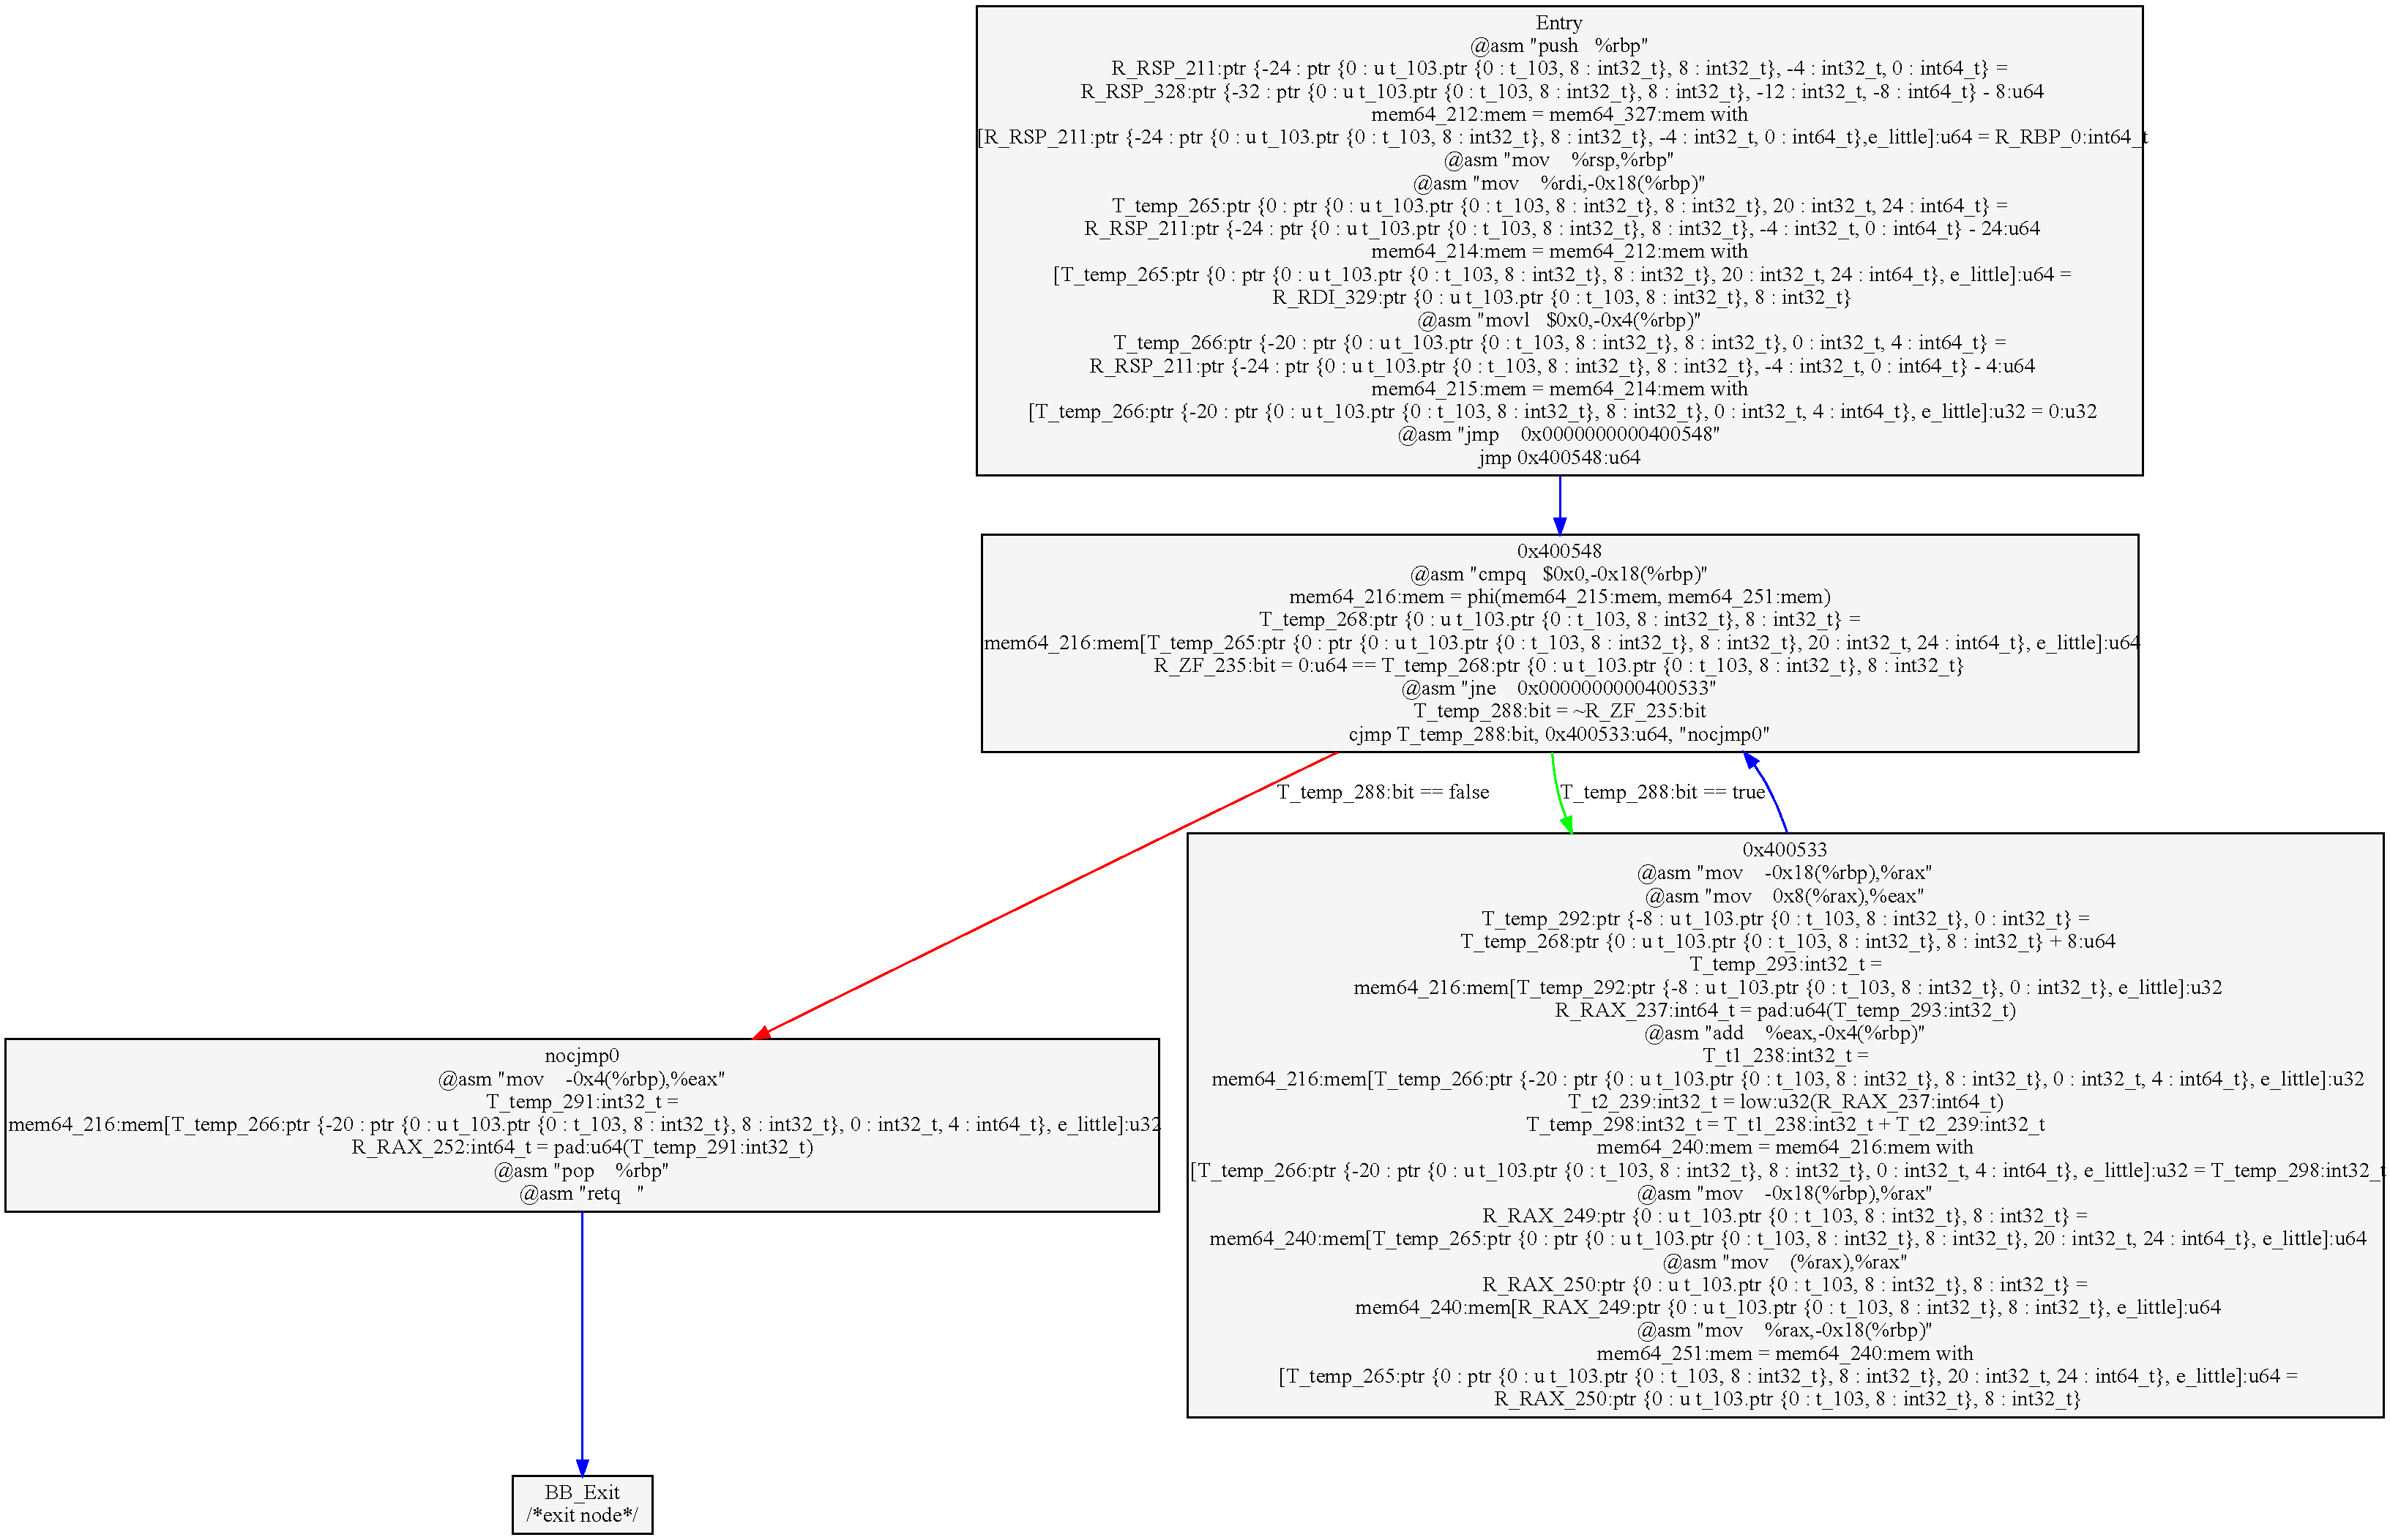
\includegraphics[scale=0.40,angle=90]{bitr/out2.pdf}
}
\caption{Solved List Summation}
\label{fig:solvedlist}
\end{figure*}


\newcommand{\tachyon}{\textsc{Tachyon}\xspace}
\chapter{\tachyon: Tandem Execution for Efficient Live Patch Testing}
\newcommand{\allsystemcallreplay}{patil:2010,guo:2008}
\newcommand{\allinstructionlevelreplay}{patil:2010,gdb,undodb}
\newcommand{\allvmreplay}{retrace,simics,vmware-replay}
\newcommand{\patched}{P}
\newcommand{\unpatched}{P'}
\newcommand{\tuple}[3]{\langle #1, #2, #3 \rangle}
\newcommand{\size}[1]{|#1|}
\newcommand{\len}[1]{\mathsf{len}(#1)}
\newcommand{\seqlen}[1]{\mathsf{seqlen}(#1)}
\newcommand{\impl}{\rightarrow}
\newcommand{\etal}{et al.\ }

In order to show that Holmes can be used in practice, we implement a concrete system with it.
We chose to focus on the problem of use-after-free, as it is a little-explored area for static binary analysis.
We used Holmes here to link together control flow analysis, alias analysis, string recovery, and general function loading in order to build a working use-after-free engine.

% Use after free bugs are common
There were 238 use-after-free (UaF) vulnerability disclosures (CWE-416) issued in 2017 alone, with 36.2\% given a critical security
rating.
% From cvedetails.com, mitre doesn't seem to issue CVE/CWE associations.
Use-after-free bugs happen when a pointer has been freed and the memory pointed to subsequently written to or read from.
Use-after-free bugs can lead to DoS, control flow hijack, and information leaks.

Despite the number of CVEs, few tools exist that can automatically and statically detect such bugs in off-the-shelf \emph{binary} code.
However, there are tools for finding such bugs in \emph{source} code.
Requiring source code limits the applicability of these techniques to developers with full source access.

In this chapter, we focus on the question
``Can we use \sysname\ to bridge the gap between analysis for UaF bugs in source code versus compiled code?''
In particular, previous work has been unable to apply source code techniques to compiled code.
Can we adapt such techniques to be effective even without source?

At a high level, UaF bugs require reasoning about memory allocation and memory aliasing.
Source code techniques are more plentiful due to the rich and mature research area of alias, points-to, and similar schemes for reasoning about memory over the lifetime of a program.
In comparison, at the binary level the primary approach for reasoning about memory is Value Set Analysis~\cite{vsa}, which is less mature and has several limitations in practice such as inability to reason about all arithmetic operations (e.g., bit-shifts and division) and the fact it may not terminate without ad-hoc widening in the presence of loops.
For example, GUEB~\cite{gueb} was proposed to detect UaF bugs using VSA, but is handicapped by disallowing cyclic paths to allow rapid termination of VSA.

We present a new binary-level static analysis approach for detecting UaF bugs in executable programs.
One of the main technical challenges we address is showing how to adapt source-code memory alias analysis to compiled code, where previous work has instead created all-new binary-only approaches to alias
analysis like VSA.
We experiment with two classes of analysis: flow insensitive alias analysis via a Steensgaard-type~\cite{steensgaard-alias} algorithm, and  flow-sensitive alias analysis using a data flow approach adapted from Andersen~\cite{andersen} style analysis with added rules to handle binary-specific details such as calling conventions and computed addresses.
We also add context-sensitivity by allowing the analysis to reason about the call-stack discipline followed by executable code, and a type of field sensitivity appropriate for direct pointer arithmetic without type information.
To the best of our knowledge, very little work has been done in applying the literature in source alias analysis to compiled code, and no previous work has shown how to then use such techniques to find UaF bugs statically in compiled code.

We have built a tool called \aliasname\ that uses \sysname\ to drive the different levels and co-dependencies in binary analysis, alias analysis, and UaF detection.
Taking this approach allows us to have an end-to-end reasoning chain from input binary to why this particular candidate use-after-free could not be disproven with a given sensitivity.

We evaluated \aliasname\ over 7 real CVEs and the Juliet test suite released by IARPA for purposes of verifying our detection capabilities and measuring false positives in the face of bugs.
Additionally, we measured false positive rates against a background of expected-good binaries (we assume no true positives): a random sampling from the \texttt{\$PATH} of a default Ubuntu installation.

\aliasname\ is available at \url{https://github.com/maurer/marduk}.

\section{Design of \tachyon}



\subsection{Overview of \tachyon and Challenges}

\begin{figure}
  \centering
  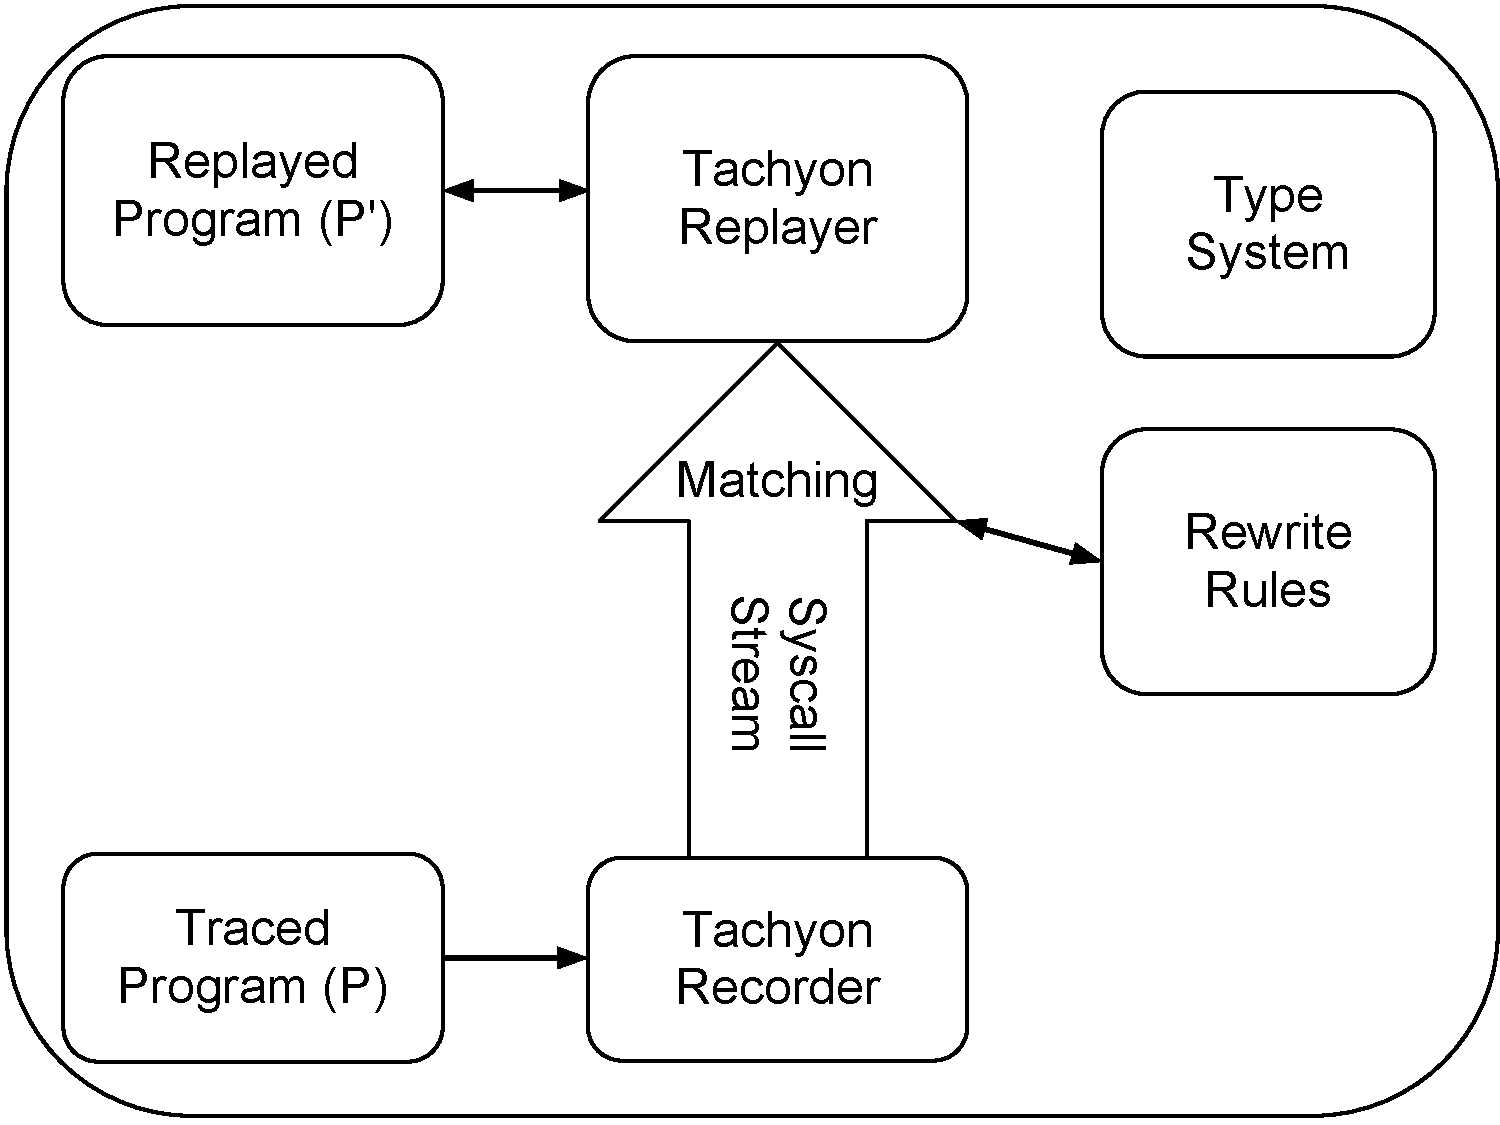
\includegraphics[scale=0.5]{tachyon/TachyonDiagram.pdf}
  \caption{Tachyon System Overview}
  \label{tach:fig:system}
\end{figure}

The overall architecture of \tachyon is shown in
Figure~\ref{tach:fig:system}.
We will refer to the program running
live  as $\patched$ (e.g., the patched program) and the program running
in-tandem with simulated syscalls as $\unpatched$ (e.g., the unpatched
program).  \tachyon is a user-land program that utilizes the Linux
ptrace facility to interpose on syscalls issued by $\patched$ and
$\unpatched$.  Like replay schemes, \tachyon has a recorder and a
replay module. The recorder records the stream of system calls
issued by $\patched$ and outputs a stream of tuples
$\tuple{C}{\vec{I}}{\vec{O}}$ where $C$ is the system call number,
$\vec{I}$ is a list of inputs to the system call, and $\vec{O}$ is a
list of outputs.  The replay module interposes on $\unpatched$, and
for each syscall $C$ with arguments $\vec{I}$ made by $\unpatched$,
simulates the OS by returning $\vec{O}$.

\begin{lstlisting}[float,caption={Example patch},label={tach:lst:example}]
-int fd = open("/tmp/fileA", O_RDONLY);
+int fd = open("/tmp/fileB", O_RDWR);
-int *storage = malloc(...);
-/* ... Do some processing with storage..  */
+fstat(fd, statBuf);
 char* incoming = malloc(chunksize);
 ssize_t size = read(fd, incoming, chunksize);
 if (size != -1)
   write(fdOut, incoming, size);
\end{lstlisting}

Consider the example shown in Listing~\ref{tach:lst:example}, with the
patch difference being displayed in diff style with full context. The first
edit changes the file opened from \texttt{/tmp/fileA} to
\texttt{/tmp/fileB}. The next few edits remove an unneeded call to
{\tt malloc}, and add {\tt fstat}.  The rest of the program is the
same. Note that since a {\tt malloc} call was removed, the returned
memory chunk for {\tt incoming} will be at a different address, even
on systems with a deterministic memory layout.  Overall, this patch
example illustrates three challenges: patches may change arguments to
system calls, may change system calls issued, may change memory
allocation patterns, and any of these changes may have effects on subsequent
execution.

% Essentially, we see here an earlier bit of processing which used an allocation
% was removed, along with an unneeded \texttt{fstat}. The call to \texttt{write}
% emphasizes the challenge of isolation for tandem execution, as a bad program
% would clobber the output of the good program. The change in allocations between
% the two moves the memory layout around, making memory diffing techniques
% ineffective for recording effects, emphasizing the second challenge. Finally,
% the spurious \texttt{fstat} which is dropped in the patch should be accepted,
% showing the need for a system call stream rewriting.


The above challenges motivate three main requirements of live patch
testing as distinguished from a normal replay system. First, instead
of offline replay, a live patch testing solution should be
\emph{online} where $\patched$ produces the syscall stream that
$\unpatched$ should consume.  Second, a live patch tester should not
depend upon pointers because absolute memory addresses may change
between runs. For example, $\unpatched$ and $\patched$ may issue
calls to {\tt malloc} for different amounts or ASLR may be enabled.
Either case prevents patch testing. As a result, we cannot determine
$\vec{O}$ by simply diffing the memory state
before and after a syscall, as in previous syscall replay
schemes~\cite{\allsystemcallreplay}.  Additionally, memory diffing
does not allow us to determine the inputs $\vec{I}$ to system
calls. As a good live patch tester should verify the inputs as well,
we need some way to extract all inputs of a system call. Without a
semantic model, we will be unable to both locate all the relevant
components of the input, and to avoid capturing irrelevant components.
Thus, we need a semantic model of the inputs. Third, since a patch
may remove or add system calls, the live patch testing scheme should
allow for the syscall stream to be rewritten during replay. This can be accounted for by allowing
rewriting of the tuple stream $\tuple{C}{\vec{I}}{\vec{O}}$.  


\subsection{System Calls and Side-Effects}

\tachyon needs to determine what the semantic inputs and outputs
to a syscall are in order to record and replay them.  Specifically, it needs to (1) determine the types of
arguments to a syscall, (2) differentiate input from
output, and (3) pointers from the pointed-to data. While existing C
syscall prototypes are sufficient  for (1), they do not provide enough
information for (2) and (3). Consider the
\texttt{read} syscall declaration:
\begin{lstlisting}
ssize_t read(int fd, void *buf, size_t count);
\end{lstlisting}

This C declaration misses crucial information.  First, it
gives no clue how the void pointer buf works. How big is it? Is it
null-terminated? Are the contents relevant before the call, after, or
both? We need to answer all these questions in order to copy the
appropriate semantic data.  We can see that even the assertion that a
pointer points at some data before or after the system call is not the
case, as with \texttt{sbrk} (pointer points at the end of your address space)
 and \texttt{mmap} (one pointer is only a suggestion). {\tt read} is one of the
simple cases; several syscalls have complicated dependencies between
input and output parameters, as will be discussed later in~\S\ref{tach:sec:types}.

\tachyon addresses the challenges associated with understanding the
syscall semantics by adding type annotations, as described in~\S\ref{tach:sec:types}. The \tachyon 
annotation language is a light-weight dependent type system that says
how to parse the inputs and arguments into semantic data at runtime.
These type annotations only need to be written once per system call,
and are portable across systems with the same syscall signatures.

\subsection{Syscall Stream Rewriting}

%\edissue{Maurer: Done. Honestly, I liked cURL better, but I understand trying to have a single example for the section.}

Many patches also change the sequence of syscalls made in addition to
the actual parameters.  Consider Listing~\ref{tach:lst:example}.  The
system call stream when executing the patched program is $\langle ...,
{\tt open}, {\tt fstat}, {\tt read}, {\tt write}, ...\rangle$.
However, the call after {\tt open}  in the unpatched program is {\tt
  read}, not {\tt fstat}.  

%Thus, the two programs have semantically
%different behavior, which we will report as a deviation.



New patched versions often have new system call patterns that cause
the program to behave differently at an IO level. It is not possible
to tell whether a particular change in system call patterns is valid
without a human to validate it. For example, if it turns out the
above code is just shifting a few things around and adding a new
inconsequential call to \texttt{fstat}, then the user may want to
ignore the deviation.  However, the \texttt{fstat} may have been
inserted for security, and a deviation may indicate an attack.  When
opening files in \texttt{/tmp/} a common security practice is to
then call \texttt{fstat} to obtain the user ID and group ID of the
file to make sure they are correct in order to detect race
conditions. \tachyon should report the deviation and halt execution in
such instances. 

Although we cannot automatically decide which deviations matter,
\tachyon does \emph{automate finding deviations}, as well as provide a
mechanism to ignore such deviations when found to continue testing.
The rewriting engine relies upon rules that are created for each
patched program that detail how to handle semantic differences. For
example, if a system administrator decides the above deviation is
inconsequential a rule can be written to ignore the {\tt fstat} call.
Alternatively, patch creators could write such rules and distribute
them with their patches to aid testing.

\subsection{Road Map}
In the rest of this chapter, we first describe the \tachyon type system in detail. We
then discuss how \tachyon rewrites system calls, as well as some
common rules we have found in patches we have tested. We next describe
our implementation and evaluation. We finally discuss several
applications of \tachyon outside automated patch testing.


%%% Local Variables: 
%%% mode: latex
%%% TeX-master: "paper"
%%% End: 

\section{System Call Types}
\label{tach:sec:types}

The C function declarations for syscalls do not describe all
side-effects. \tachyon proposes an extension to the C type
declarations to encode all semantic information necessary to record
which parameters are inputs, which are outputs, and how to identify
all bytes for each parameter. While this problem has been attacked before~\cite{guo:2008},
our particular needs are different due to the binary only-nature of our
approach, as we discuss in \S~\ref{tach:sec:related}.

The \tachyon type system takes advantage of the
user-space/kernel-space barrier for interposition. The barrier
provides a clean separation that can be monitored without
requiring source to the program. In addition, the barrier allows
\tachyon to not monitor internal kernel state. The reason is that the only
way $\unpatched$ and $\patched$ can interact with the underlying
system is via \tachyon, and \tachyon's mechanism ensures that both
programs see an identical state.  This is a vital complexity
reduction.

\tachyon uses a limited form of lightweight dependent types (types
which depend on values). Our lightweight use avoids pitfalls such as
undecidability normally associated with dependent types. In the rest
of this section, we first provide an intuition on the issues and how
dependent types are used, and then describe the full system.


\subsection{Intuition}

A basic approach for recording syscalls is to decorate C types with
information about which parameters should be treated as inputs,
outputs, or both.  We call such annotations the IO class for each
parameter.  In order to specify how to copy output parameters, we also
need to know the size of their values.  The size information is needed
because we need to copy all output bytes from {\tt buf} in the
monitored program $\patched$ to the address space of $\unpatched$.
For example, we could imagine annotating the {\tt read} call as:
\begin{lstlisting}
ssize_t read(int fd, void output* buf{ret}, size_t count);
\end{lstlisting}
The parameter {\tt buf} has been annotated as an output parameter,
thus should be copied and replayed to $\unpatched$.  The annotation
also specifies that {\tt ret} bytes should be copied, where {\tt ret}
is the return value.


Unfortunately, such simple annotations are insufficient with many data
structures, such as vectors. A prime example of a difficult system
call is \texttt{readv}, which provides vectored reads of a file
descriptor. Its C type declaration is:
\begin{lstlisting}
ssize_t readv(int fd, const struct iovec *iov, int iovcnt);
struct iovec {
  void  *iov_base; /* Starting address */
  size_t iov_len; /* Num bytes in iov_base */
};
\end{lstlisting}
The main issue demonstrated is that a complete description of the IO behavior of
parameters may refer to other parameters.  The {\tt iov\_base} length
is determined by {\tt iov\_len}, and the total number of {\tt iov}
items is given by {\tt iovcnt}.  \texttt{readv} is not alone: it has
many friends such as \texttt{writev}, \texttt{preadv}, and
\texttt{pwritev}. In order to handle such cases, we need a type system
that allows us to express \emph{relationships} between parameter values.

% Suddenly, it is less clear exactly how to encode this, and this system
% call is not alone, there are a number of others like it, though it
% and its friends 
% are somewhat unique in that they exercise three cases not addressed by the
% previous system (pointers not in an argument, sizes not in an argument,
% and variable numbers of pointers). In particular, we are now on to a more
% dependent type system, as the exact type is dependent upon a function of the
% values, e.g., the size of the buffer pointed at by \texttt{iov\_base} is
% determined by the lenth next to it.


\begin{figure}
	\begin{center}
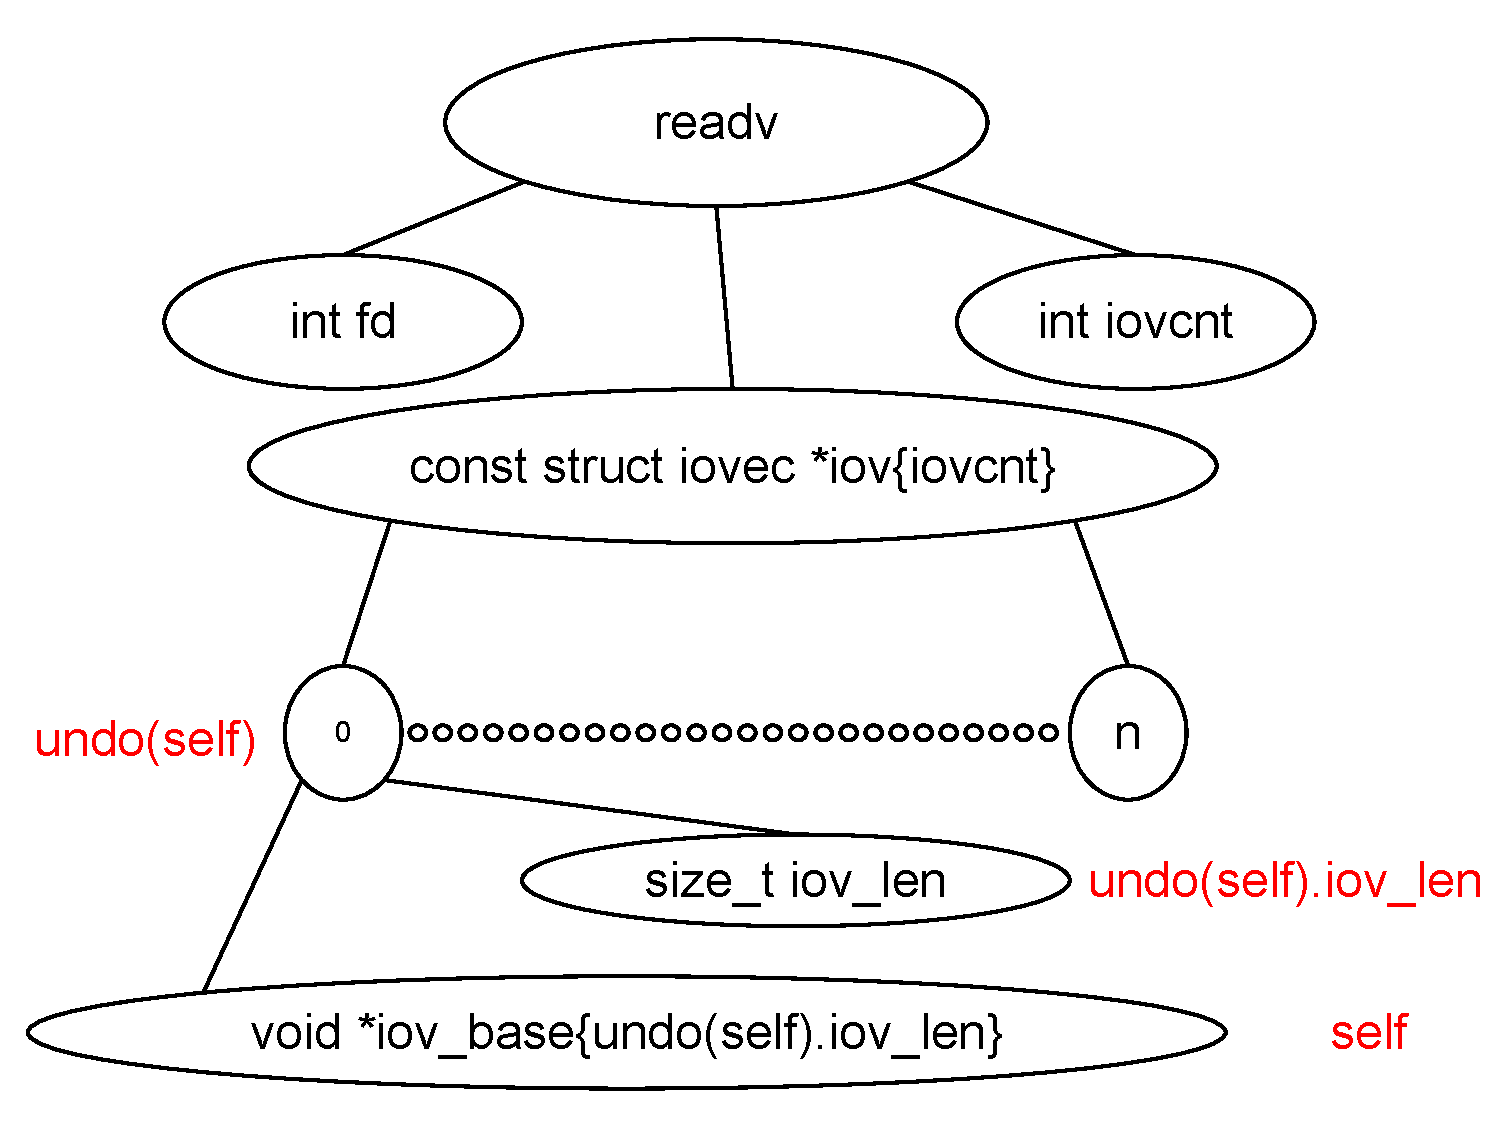
\includegraphics[scale=0.4]{tachyon/LookupDiagram.pdf}
	\end{center}
\caption{A lookup in action}
\label{tach:fig:lookup}
\end{figure}


\tachyon uses lightweight dependent types that can express
relationships between the value of one parameter and the value of
another.  We view types as a tree, and use dependent types to walk the
tree to determine a value.  


The types allow us to walk from the top of the tree, or from the
current parameter.  In \tachyon, we specify {\tt readv} as:
\begin{lstlisting}
ssize_t readv(int fd, const struct inputoutput iovecin *iov{iovcnt}, int iovcnt);
struct iovecin {
  void input *iov_base{undo(self).iov_len};
  size_t iov_len;
}
\end{lstlisting}
We now call the struct \texttt{iovecin}, because while both
\texttt{readv} and \texttt{writev} take an \texttt{iovec}, they are
used differently, and so are assigned differing types (specifically,
in one case the buffers inside are output, while in the other they
are input).  The only new annotations compared to before are
\texttt{undo} and \texttt{self}, which are used to walk the type
tree to reference other fields. The semantic meaning is that
\texttt{iov\_base} is \texttt{iov\_len} bytes.  \texttt{self} refers
to the location at which the current value is being read from.
\texttt{undo} simply says to step back along whatever indexing step
was done to get there.  In this case, this means that \texttt{self}
represents the tree traversal up through that instance of
\texttt{iov\_base}. The ``undo'' brings us up a level, to be looking
at the struct. Then, we index the struct to \texttt{iov\_len} and are
done.  Figure~\ref{tach:fig:lookup} graphically shows the type tree for
\texttt{readv} and how the syntax expresses fields in the tree.

% This is useful as a point of
%reference so that structs can have self contained types, allowing for
%reuse across functions (and can exist in arrays like the one we have
%here).


\subsection{The Tachyon Type System}
The full \tachyon dependent type system is shown in
Figure~\ref{tach:fig:annotations}, and is taken directly from the \tachyon
source code in Haskell.  The language is similar to BNF, where
non-terminals are to the left of the equal sign, and brackets denote
a list (e.g., [A] is a list with elements of type A).


\begin{figure}
\lstset{language=Haskell}
\begin{lstlisting}
data SysSig = SysSig Type [Type]
data Type = Small Int
          | Struct [Type]
          | Ptr IOC Type Bound T
data T = NT | UT
data IOC = In | Out | InOut
data Bound = Const Int | Lookup Lookup
data Lookup = Ret | Arg Int | Index Int Lookup | Self | Undo Lookup
\end{lstlisting}
\caption{The \tachyon annotation language}
\label{tach:fig:annotations}
\end{figure}

In \tachyon's language, IOC represents an IO class, that is, whether
the pointer is input, output, or both.  T represents some form of
termination, to allow us to include null-terminated data. NT is for
null-terminated data; UT is for unterminated data. If a pointer is
null-terminated, reading will cease when a 0 is hit, if this happens prior
to the end of the buffer. The index operation is used on both arrays
and structs, where the $i$'th index refers to the $i$'th field
(counting from 0).

The types available are
\begin{itemize}
\item Small - These correspond to basic integer C types, like
  \texttt{char} or \texttt{long}, and indicate values that should not
  be treated as pointers. The type parameter is the number of bytes of
  the type, e.g., Small(1) is a 1-byte value corresponding to a {\tt
    char}.

\item Struct - an aggregate of other types. Note that previous replay
  work treated such types as raw buffers because they could determine
  size by simply diffing memory before and after a syscall.  In live
  replay, we explicitly lay out all fields because the underlying
  types may yield further information.

\item Ptr - a pointer  annotated with an IO class, the type of
  element it is pointing to, a way to tell how many elements it points
  to, and whether or not it respects a null termination convention.
\end{itemize}

We introduce the concept
of a ``lookup''. This is just a series of steps that can be performed
from either the arguments of a function in the case of an input or
in/out class pointer, or the arguments and return value in the case of
an output pointer, to arrive at a memory location or register. This is
demonstrated in Figure~\ref{tach:fig:lookup}. The Ret and Arg
constructs for a lookup are used to allow us to reference the return
value or various arguments in a system call, respectively.  This is
just the generalization of the tree walking described earlier.

Given this, the encoding of a bound as either a constant or a lookup
is rather natural. It is the use of this bound that makes us lightly
dependently typed---the type depends on the data in question.

Finally, we can build the fundamental structure all this is for---the
system signature.  A system signature, indicated by SysSig, is what is
assigned to each system call in order to allow the tracer to
record and play back its effects. The first parameter is the type of
the return value, and the second is a list of the types of its
arguments.

\paragraph{Type Checking \tachyon Declarations.}

The \tachyon types need only be written once for each system call,
and can be reused for any program.  However, since they are written
manually, we would like to prevent mistakes.  In order to achieve
this, \tachyon also provides type-checking to make sure the
annotations make sense. In particular, \tachyon checks:
\begin{enumerate}
\item Bounds are numbers, not pointers or something else.
\item Bounds use only information which is available for the IO class of the pointer (e.g., input class may not use the return value as a size).
\item Output pointers do not contain structure; they are raw data.
\item Types are potentially compatible with the original C type.
\end{enumerate}
These checks ensure annotations which are usable, self-consistent, and match
the C type. 


%%% Local Variables: 
%%% mode: latex
%%% TeX-master: "paper"
%%% End: 

\section{System Call Stream Deviation Detection and Rewriting}
\label{tach:sec:equiv}

Patches often add, delete, or modify  new system calls in the original
buggy program.  Our example in Listing~\ref{tach:lst:example} shows all
three cases.  When the streams of syscalls differ, then the two programs are
semantically different.  While this means we cannot automatically tell
if the differences are meaningful, we can (a) automatically detect
deviations and (b) rewrite deviations when informed by the user that
the semantic differences are permitted. The heart of detection and
rewriting is \tachyon's syscall stream matching and rewriting engine.

% When the syscalls change between$\patched$ and
% $\unpatched$, then 

% Since the patch introduces semantically different I/O, it is
% impossible to automatically decide whether the changes are
% inconsequential or not. However, we can (a) automatically
% \emph{detect} 

% Naively, you might expect that pre and post-patch programs will always
% issue the same set of system calls on normal inputs.
% Unfortunately, this is not the case.
% For example, if a program changes the size of the
% buffer in a bulk transfer from 1024 to 4096, this will
% cause a change in the system call stream (fewer read/write calls), while causing
% little or no change in the effects.

\subsection{Stream Matching}

\tachyon uses a rule-based system for rewriting
system call streams during execution, designed to be employed by a
user of the tracing software to explain to the system what behaviors
it should consider equivalent. The rules must consume a sequence of system calls by
$\patched$, and produce a corresponding set of system calls for $\unpatched$ to
make in order to allow for writing call results into $\unpatched$ and checking
that $\unpatched$ indeed matches the particular equivalence rule.

As we execute, we have two streams of tuples. \tachyon represents the
stream from $\patched$ as $\tuple{C_i}{\vec{I}_i}{\vec{O}_i}$, and the
stream from $\unpatched$ as $\tuple{C'_i}{\vec{I}'_i}{\vec{O}'_i}$.
The easy case is when the two programs are semantically equivalent by
issuing the same system calls, i.e., $\forall i: C_i = C'_i \land \vec{I}_i = \vec{I}'_i$.  In this case no rule is needed, and
\tachyon will send the corresponding $\vec{O}_i$ for each $\vec{I}_i$ to $\unpatched$.

Any time the syscall input arguments do not line up, \tachyon reports a
semantic deviation.  In order to permit some deviations, \tachyon
provides the ability to rewrite the system call stream.  The rewrite
engine takes in a set of rewriting rules $f$.  Each rewrite rule $f_k$
is a function which takes in $\tuple{C_i}{\vec{I}_i}{\vec{O}_i}$ and
$\langle C_i', \vec{I}'_i \rangle$. 
The rule uses pattern matching
to decide if it applies, and if so, returns a pair of equivalent syscall
streams to perform a substitution with.
After a
match, the stream continues to be consumed by the simulated program $\unpatched$. 

% In the simplest case, each sub-stream is of length 1, and so we
% get a deletion sub-stream that looks like
% $\tuple{C_i}{\vec{I}_i}{\vec{O}_i}$, and an insertion sub-stream that
% looks like $\tuple{C'_i}{\vec{I}'_i}{\vec{O}'_i}$, where $\vec{O}'_i$
% is generated by the function in question.

The overall mechanism can be used for:
\begin{itemize}
\item Determining roughly equivalent  syscalls, e.g., many small
  writes being patched to be one big rewrite.
\item Ignoring syscalls, e.g., the $\patched$ program issues a call
  that is not needed by $\unpatched$. 
\item Limited reordering, e.g., allowing for syscalls to be switched.
\end{itemize}


%\edissue{You suggested this section needed to be rewritten for clarity. Have these changes done the trick?}


\subsection{Rewriting Rules}

Each rewrite rule $f$ takes a system call (the one made by $\patched$)
and the input to a potential system call made by $\unpatched$, and
returns a substitution in the stream. The substitution is implemented
as a pair of lists, where the left list indicates the syscalls
consumed by the rule, and the right list indicates the corresponding
substitution produced by the rule.  The type signature for $f$ in
\tachyon is:
\[
\text{Syscall}  \impl \text{SysReq} \impl \text{Maybe ([Syscall],
  [Syscall])}
\]
\noindent where the ``$\text{Maybe}$'' indicates that the rule may also return that
no substitution was performed. 


The rewriting rules are pure functions, which means they have no
access to outside resources like the current syscall stream or
application state.  By being pure we ensure that rewrite rules can be
applied in any order.  In addition, it ensures that the rule engine
itself will not continually accumulate state, i.e., while individual
rewrites may take substantial space, the space used will remain
constant in the number of system calls which have gone through, which
is vital to an online system.


During execution, the matching engine maintains a queue of syscalls
executed by the live program $\patched$.  Suppose the queue contains
any syscall $x$ that is not \texttt{write}, but the simulated program
$\unpatched$ issues a \texttt{write} syscall.  The simplest rule is to
ignore the \texttt{write}.  This is accomplished by adding a
\texttt{write} to the queue before $x$.  When the matching engine
re-examines the queue, it will match the still-pending \texttt{write} to the
one in the queue, and not report a deviation.

In \tachyon, the rule is written as:
\lstset{language=Haskell}
\begin{lstlisting}
ignoreWrite :: Syscall
            -> SysReq
            -> Maybe ([Syscall], [Syscall])
ignoreWrite x (Write 2 buf sz) =
  Just ([x],
        [Syscall (Write 2 buf sz) sz, x])
ignoreWrite _ _ = Nothing
\end{lstlisting}

This rule fires when line 4 is matched. This occurs when $\patched$
issues a syscall $x$ that doesn't match $\unpatched$'s syscall
\texttt{write}. On line 5 the rule directs it to consume whatever is
on the stream at the moment, and replace it on line 6 with the stream
of \texttt{Write} followed by $x$. This can be thought of as
``faking'' the call for \texttt{Write} to the stream matcher so that
it does not report a deviation. On line
7, we catch the case where our conditions are not met, and
indicate we did not modify the stream.

The simple, no-look-behind method of replaying with this equivalence
is to replay the stream normally until a match fails. At this point,
the two syscalls that failed to match are fed into all rewrite rules,
and their replacement list for the original stream is checked. If
there is still more than one rewrite rule remaining, one is chosen
arbitrarily. In future work, checkpointing could be used here to allow
for the ability to rewind if the wrong replacement was chosen.  In
practice, the rules we tested have only yielded one matching rewrite.

%In this way, we can safely describe a looser form of equivalence that
%still allows for the replaying of the new system call results to the
%program, and so allows us to continue the trace.


A more complex example is what we call write splitting, which occurs
when a larger write in the original program is translated into two smaller writes in the
replayed program. This is useful if the buffer size used in a
transmission was decreased during the patch, as it allows for a roughly
equivalent operation---writing one part of the message, then the other---to
be treated the same as the original system call writing the entire
message. A concrete example would the difference between the program fragments:
\begin{lstlisting}
-#define CHUNK 4096
+#define CHUNK 1024
 while(buf < end) {
   buf += write(fd, buf, min(end - buf, CHUNK));
 }
\end{lstlisting}

In the patched case here, we will see on average 4 times as many
system calls, but fundamentally, the same thing is happening. A
rewriting rule for write splitting says that a sequence of previous
writes can be used to fill on big write request:
\lstset{language=Haskell}
\begin{lstlisting}
writeSplit :: Syscall
           -> SysReq
           -> Maybe ([Syscall], [Syscall])
writeSplit (Syscall (Write fd buf sz0) sz) --sz is return size
           (Write fd' buf' sz')
 | (fd == fd')
  && (sz' < sz)
  && ((take sz' buf) == buf')
     = Just ([Syscall (Write fd buf sz0) sz],
             [Syscall (Write fd' buf' sz') sz',
              Syscall (Write fd' (drop sz' buf)
                                 (sz0 - sz'))
                        (sz - sz'))
writeSplit _ _ = Nothing
\end{lstlisting}

This rule states that if we have a write call in the original
stream, and the replayed program is trying to make a non-matching
write call, but it matches on the file descriptor, and has a smaller
size, and the write it is trying to make is a prefix of the original
write, then we can replace the original write with two smaller writes,
the first of which is the target write, and the second of which is set
up to represent the rest of the write.

In line 6, we do a sanity check that the file descriptors we are
writing to are the same, followed by a similar check in line 7 that
the request from $\unpatched$ has a smaller size than the original
form $\patched$. Finally, in line 8 we make sure that what is trying to be
written is a prefix of the appropriate length of the original write.
Given these conditions, we know that we can provide a replacement rule
which will allow the trace to proceed. In line 9, it tells its caller
to consume the most recent call, asserting that it matches the call
passed into us. In line 10, we see the first call that is going to end up
on the new stream, which matches the input vector we've received from
$\unpatched$, and so will allow the trace to continue. In the 11,12,
and 13, the function returns an additional item for the system call
stream, which represents the rest of the write that has been split.
In 14, we catch the case where we don't apply, and simply return no
pattern.


%%% Local Variables: 
%%% mode: latex
%%% TeX-master: "paper"
%%% End: 

\section{Implementation}
\label{holmes:sec:impl}
In order to evaluate the language as a means towards program analysis, we need a running implementation.
\subsection{Holmes (Old Implementation)}
Initially, I produced a database backed implementation which compiled down to a combination of Rust and SQL (initially C++ and SQL) and had Postgres handle joins, deduplication, and data storage.
This had the advantage of being able to handle significantly larger working sets in theory, but in practice had significant performance issues which lead me to change approaches.
Despite this, I feel it is worth discussing here both because the failures of the implementation point out some of the unique challenges and simplifications that can be made in evaluating datalog, but also because it seems inevitable that to analyze programs substantially larger than those examined in this thesis, either a distributed platform or a disk-backed system will need to be used.
It is my hope that these lessons learned will help a future external-database based implementor avoid the same pitfalls.
Most of the details here are focused on Postgres, but other systems take a generally similar approach so similar problems are likely to occur.

As a result, this section is mostly focused on what went wrong, rather than on how the system was constructed.
If you want to see how the system was constructed, source is available at \url{https://github.com/maurer/holmes}, but be aware that it does not represent a complete implementation of the language.
In particular, it only has partial support for aggregation, and no support for circumscription.

\subsubsection{Indices}
% Which indexes to make?
%TODO cite postgres/mysql/mssql?
Database software usually does not know which indices would be ideal to keep, and since keeping extra indices is is expensive in both time and disk, most SQL systems require the user to specify the indices to keep manually.
Work is ongoing~\cite{peloton} to remedy this problem, but is not yet a production tool.
In the meantime, if we wish our translated datalog queries to run efficiently, the database must be provided with a list of indices to keep.

We tried a number of heuristics, including indexing in a global attribute ordering, indexing per query based on left-to-right joins, and just indexing all fields in order, and having the programmer reorder fields to boost performance.
None of these approaches worked in practice.
Both the global ordering and the left-to-right joins failed in large part because the query planner would choose to reorder the joins at runtime in multiple different ways.
The programmer manually ordering fields could find local optima, but because predicates are used in multiple ways, it too falls short.

The solution in use at the time this approach was switched away from was to annotate the program with an explicit set of indexes to keep.
We generated these indices by profiling the running program, and adding indices which would allow the query planner to avoid nested loops or full table scans where possible.

\subsubsection{Append-Only, High Write}
% Append only workload
One interesting aspect of a datalog system that the workload is entirely append-only other than retraction events, which are intended to be rare.
This knowledge is unused by the database in executing queries.
If it materializes a view to execute a query, and an underlying table is updated by an append, it will re-materialize the whole view, not perform any kind of incremental maintenance.

One of the expensive parts of many queries was insisting that it only return results which contained at least one \emph{new} fact - one which hadn't been returned in this query before.
That tables can only be appended to could enable the incremental maintenance of the join, allowing more efficient computation of the join, and retrieval of only the new data.

There are also some database schemas (such as the star schema) which become more possible in the absence of mutation or deletion.
\subsubsection{Query Planning}
Query planning, while of benefit to users who do not know all their SQL ahead of time, or whose tables remain in steady states, was the biggest issue with this approach.
Databases commonly use a component called a query planner to translate SQL statements into an internal representation (loops, merge joins, hash joins, index walks, etc) that they can concretely execute.
This component depends on a variety of information, including but not limited to:
\begin{itemize}
	\item Whether the statement was prepared
	\item If prepared, how many times it has been executed
	\item What indices are available
	\item Information from the statistics daemon
\end{itemize}
Other than examinining what indices are available, these conditions turn out to be highly anti-productive for a datalog workload.

The statistics daemon is designed with the assumption that there is a sort of ``steady state'' for a database, in which the relative sizes of the tables will remain similar.
This makes sense for usual customers of databases, but in our case, a large part of operation looks like heavy insert activity on a specific table.
As a result, the statistics daemon's information is generally woefully out of date.

We prepare virtually all statements, since we intend to execute them repeatedly and want to avoid time in the parser.
However, as of the time this system was developed, postgres would ossify the query plan as of the 5th time a prepared statement was executed.
This was done based on the assumptions that SQL connections do not live so long that the database changes a lot, so by the fifth time the query is run, the plan is unlikely to be improved, and performance will be increased by avoiding the planner entirely.
In practice, this means that any recursive rule (like one marking nodes as reachable, or performing a dataflow) will have suboptimal performance.
The rule executes five times, and during that time, the statistics daemon either has old out of date information, or even if it updates, information that the table it's reading out of is terribly small.
The query planner then makes bad decisions based on this, then sets them in stone.
As a result, indices sit there unused, and logarithmic operations are done linearly.

If the statements are not prepared, we incur parsing and planning overhead on every query.
While unfortunate, those costs were low in comparison to the troublesome queries.
The true problem with completely non-prepared statements is that the query planner would rapidly change strategies, meaning that which indices are needed would change at different points in execution.

Since in our case we have a fixed query set and a rapidly changing database, it would most likely make more sense to absorb the query planner into the compilation process somehow.
Postgres did not at the time of implementation have a way for a client to provide it with an explicit query plan short of building and providing a plugin which ran said plan as a function.

\subsubsection{Star Schema}
%TODO: note that this is equivalent to picking a good $I$ for our model, finding it, then swapping it back to Herbrand at the end
As alluded to earlier, one benefit of an append-only workload is that star schemas have lower overhead, as garbage collecting the child tables is not necessary.
Star schemas are normally used for ``data warehousing'', a sort of large scale database where an organization's data is all loaded into a single schema before being pulled out again into smaller databases for actual processing.
The idea is that most values are referenced rather than included directly in tables.
Warehousing personell are largely interested in the standardization of these values and the resulting compression.

In our case, a star schema is interesting both for reasons of compression, and for ease of indexing.
Indexing an IL instruction sequence\footnote{
IL instruction sequence refers to a lifted representation of an assembly instruction or sequence of assembly instructions into an "intermediate language" which as fewer, more orthogonal operations.
}, whether by hash or by ordering, is much slower than sorting by a tuple of integers.
We discovered this technique after the pivot to an in-memory database, so I have no observations of its performance, but I expect it would help.

\subsubsection{Large Objects}
With an external database, the use of large objects becomes nontrivially expensive.
If the database is local, and the bus between the program and the database is shared memory, this is not a major issue.
However, even over a local unix socket, repeated accesses to large objects can inhibit performance.

This shows up in practice when dealing with binary sections and segments during lifting.
If the lifting rule needs the segment, the architecture, and an offset into that segment to perform the lifting, this can incur several copies of the segment per instruction.
In my sample programs, most segments were between 300k and 600k bytes, causing this to incur a nontrivial cost.

The first solution, specific to this problem, was an all-at-once chunking of the segment.
We requested the segment from the database, then produced a 16-byte chunk (maximum length of an x86 instruction is 15 bytes) at every offset, and sent it back.
In the future, requests would access this chunked data rather than the original.
This resulted in a 16-17x blowup of the space to store the base binary, but as that paled in comparison to everything else it was not especially significant.

The second solution was to add another extension to datalog allowing some functions to exist as special external predicates to be run database side.
These all needed to be builtins, and while the approach was slightly more efficient, overall I no longer think the improvement warranted the complexity.

If I were to address this again today, I would use a star schema database side, and implement a cache client side for fetched star objects.

\subsection{Mycroft}
\label{sec:mycroft}
Mycroft is a row-oriented, single-threaded, in-memory datalog engine, taking into account the experiences of the initial implementation.
It operates as a macro which transforms datalog into Rust code, which can then be compiled into a running program.
In its current form, it addresses most, though not all, of the pain points encountered with Postgres.
The query planner is replaced by a single plan, generated at compile time, which parameterizes itself only on the size of the relevant tables at that moment.
This replacement also means that we know precisely what indices will be useful, and can generate them.
The join algorithm is aware of the incrementality of append only joins, and uses this to speed up requests for new results. 
As Mycroft is in process and in memory, large objects are not a problem.
They are returned as read-only references to the existing strucure, and can be operated on that way.
The implementation is available at \url{https://github.com/maurer/mycroft}, and as a crate on \texttt{crates.io} for direct inclusion in rust projects.

\subsubsection{Typed Storage}
Rather than store data values directly in rows as was done in the Postgresql-based implementation, here we keep a separate deduplication table for each type of data on which we operate.
This allows us to efficiently map back and forth between values, which the callbacks need to consume, and integer keys, which are convenient for indexing and join algorithms. 
This is reminiscent of the star schemas discussed before.
As our system is mostly-append (other than retractions due to circumscription) we design this as an insert-only structure.
An additional benefit, more relevant here than with Postgres, is that this greatly reduces our memory footprint.

At compile time, each type present in one or more predicates has a modified robin-hood hash table declared for it.
This table has two pieces: a vector backing which stores the actual data, and a vector of hash/key pairs.
There are two operations this table needs to support: acquiring the key for an object, whether or not it's present already, and acquiring an object from its key.
Finding the key for an object is accomplished by using a lookup on the hashtable portion of the structure, inserting into both the table and the vector of data in the event of a lookup failure.
Finding the object for a key (the more common case) works by indexing into the vector.

The only principal difference between this and a simpler design (a standard hash table mapping from the value to the key, and a vector mapping from a key to a value) is that it stores the data only once, and without any indirection.
While this may not sound like much, this gave a modest 23\% time performance boost over the standard library implementation in time, and approximately halved space on an earlier version of the use-after-free detector.
The closest approach still using the standard data structure would have been to use a smart pointer to share data between the data structures, or a hashtable of hashes.
The smart pointer caused trouble with the interfaces, and hashing twice incurred a performance penalty, so we used this custom hastable design for deduplication and unique key assignment.

\subsubsection{Aggregation}
As aggregation is described at the predicate level, we can implement it directly on the tuple storage.
Tuple storage is structured as a map from the tuple of non-aggregate fields (reordered to the front) to a tuple of aggregate fields.
These aggregate fields are represented by a triple of the value-keys to be aggregated, a current aggregate value, and an index indicating how many of the value-keys are aggregated in the cached value.
This allows for a lazily updated computation of the meet.

When a tuple is inserted into the store, if a value with the same non-aggregate fields is present, the value-key list is extended, but the aggregate is left alone.
If it is not present, we initialize the aggregate value with the value of the key in that slot, fill in the key in the keys-to-be-aggregated, and set the index to 1.
When retrieving a tuple, we check whether the index is equal to the length of the comprising keys.
If it is not, we start the iteration at the index, and perform iterative meets until the aggregate is up to date.
We then return the tuple, extended by the aggregate fields and reordered.

\subsubsection{Join Computation}
Datalog computation is join-heavy, and as a result attempting to compute the join naively can lead to disasterous execution times.
There are a variety of existing join approaches.
% Cite postgres?
RDBMSes tend to favor straightforward strategies, such as nested looping, hash join, and merge join.
Merge joins require a relevant index, but generally perform substantially better unless tables are extremely small.
Hash joins operate by creating an intermediate data structure of one of the tables which is indexed by the hash of the joined values.

However, for high-arity join patterns, better algorithms exist, usually formulated as ``worst-case join'' algorithms.
Ngo showed~\cite{nprr} that it is possible to develop join algorithms which are optimal even under these conditions.
This algorithm is rather complex, and is intended for theoretical results rather than actual implementation.
However, LogicBlox~\cite{logicblox} developed an algorithm known as Leapfrog Triejoin~\cite{lftj} which achieves these same bounds while remaining practically implementable over traditional indices.
Unfortunately, this algorithm is patented, and so could not be used.
This indicates a potential for future implementations to derive a novel approach from the AGM~\cite{agm} bound or Ngo's~\cite{nprr} approach, but developing such an algorithm is beyond the scope of this thesis.

In Mycroft, we used a simultaneous merge join ordered from smallest table to largest table.
An index is selected for each table which walks it in unification argument order, with constant arguments being sorted to the front.
The first index is advanced to the first tuple where all the constant arguments match.
This is made easier by the use of integer-only tuples, as the non-constant arguments can be represented as 0 in a query to the index.
Then, candidate variable bindings are made to the unification terms (if possible) and the next table is considered.
When on the last table, if a candidate set of assignments to the unification terms can be completed, it is emitted and the index advanced by one step.
If the index cannot advance or the index fails to unify with earlier tables, we know that no further result is possible, and go back one table, and continue.
This approach keeps around only a small amount of additional state, linear in the number of clauses in the query, as it is returning results.

However, due to our need for \emph{incremental} results, we can improve this mechanism substantially.
Rather than computing the entire join at once, we split it into subjoins, one for each clause in the query.
We have a separate, much smaller index for ``new'' facts in referenced predicates, requested by the query at database initialization time.
We perform a subjoin with each predicate's large index swapped for this small index to get exactly those results which we would receive that we did not before, then chain them for a result.
The small indexes are emptied during this operation, so they will not yield the same results again.

As an example, consider evaluating the query $A(x, y) \& B(y, z) \& C(z, x)$ for incremental results.
The first time it is evaluated, we perform a full join, ignoring the subjoin strategy - it would be equivalent to performing the full join 3 times.
Then, we insert two facts into $A$, and one into $C$.
Running the query again, we perform three subjoins, one on $A', B, C$, one on $A, B', C$, and one on $A, B, C'$.
In our join algorithm above, remember that we sorted the smallest table to the left.
As a result, the join with $B'$ immediately terminates, yielding no results.
For the join with $C'$, it essentially acts as a join on $A$ and $B$ only, with a constant restriction.
The join with $A'$ is similar, but the $A'$ portion of the join yields two facts, so it essentialy runs two constant constrained joins of $B$ and $C$.

\subsubsection{Provenance Tracking}
In order to later manage circumscription, or to allow a human to trace the reasoning of a program, we need to keep track of where facts come from.
To do this, in conjunction with each tuple we store a list of possible justifications.
A justification is composed of the ID of a rule, and the IDs of the facts used to match the body clause of that rule.
An aggregation is represented simply as the list of fact IDs aggregated for the match.
A map is additionally maintained from fact IDs to justifications which contain them.

\subsubsection{Circumscription, Call/CC, and Retraction}
Implementing circumscription essentially involves monitoring accessed aggregations to see if they would change, and responding with a retraction.
The previous description of aggregates does not easily allow for this.
A tuple insertion does not know if something has depended on this aggregation's completeness, and if so what.
To deal with this, if a tuple is circumscriptively fetched, we replace the list of merged keys in the aggregate field with a newly minted aggregate ID.
Three maps are maintained for aggregate IDs:
\begin{itemize}
	\item Aggregate ID to comprising Fact IDs
	\item Aggregate ID to dependent justifications
	\item Fact IDs to Aggregate IDs they comprise
\end{itemize}

If a tuple insertion occurs and would need to update an aggregate represented by an aggregate ID, that aggregate ID is retracted.
The retraction code acts as a worklist, initially populated by the broken aggregation.
First, it removes any justifications broken by the current retracted item.
Then, it retracts (by adding to the worklist) any facts which now lack justification.
If the current retracted item is a fact, it also retracts any aggregate IDs which now have one fewer fact.

In the special case where the tuple just inserted was also retracted, we replace its justification with one referencing the members of its now broken aggregate ID.
This ensures that while this justification no longer cares about the expansion of the circumscription, it will still be properly retracted if one of the facts in the original aggregate becomes invalid.

%TODO explain how we deal with cyclically supported facts
% e.g. \neg B -> A; A -> A; discover B, how do we ensure we retract A?
% Also explain how this works in the presence of circumscription.

\subsubsection{Future Work}
There is plenty of room for improvement in the concrete implementation of the language engine.

Currently, we keep more indices than are strictly necessary.
Even with our current join strategy, the count of indices kept scould be reduced through a mechanism to match attribute ordering between queries more frequently.
With a more modern join like tetris join~\cite{tetris} it could even be possible to keep a single index per predicate.

Results of some subjoins get used repeatedly, and can be known not to change through topological sorting.
Currently, this is exploited through manual tabling - the creation of dummy predicates to keep the completed join as a realized structure.
However, it should be possible to generate these temporary structures automatically in some cases.

Pivoting indices from a simple in-memory btree to a MVCC\footnote{
	MVCC stands for Multiple Version Concurrency Control.
	MVCC trees are common in database design because they map well to the block-at-a-time disk update structure and because they allow for multiple transactions to act on the same index in a way that makes it clear if the index was invalidated while using it.
	They accomplish this by retaining any portion of the tree which is being accessed by some transaction, and garbage collecting as threads leave.
	This results in "multiple versions" of the tree being accessible simultaneously in order to deal with concurrency contention, thus the name.
}-style structure would allow multiple worker threads to be evaluating rules at the same time.
As modern systems generally have additional cores, this should lead to performance improvements overall (though degradation in bottlneck phases).
This approach also meshes well with optionally backing some data structures with disk due to either large size or low traffic.
Many MVCC trees are already designed as on-disk data structures due to their use in traditional RDBMS systems.
Allowing some data to reside on disk would increase the maximum size of analysis the system could perform on a single binary, or allow for easier multi-binary analysis.

In an ideal world, this system could even be distributed.
Other than circumscription and the decision to terminate, every component of this system can operate safely with a partial knowledge of the database.
As a result, it seems plausible that with appropriate heuristics for shuffling and synchronization around circumscription, this language could be well suited for distributed execution.

\section{Evaluation}
\label{tach:sec:eval}

We have evaluated \tachyon with respect to three main
questions. First, can \tachyon detect deviations where the patched
program is semantically different than the unpatched, and how hard is
it to write rules to ignore deviations that do not matter? Second,
what is the performance factors for \tachyon, including best and worst
case settings? Third, what is the performance on real programs?  In
this section, we describe our results.

\subsection{Detecting Deviations}

To test the effectiveness of \tachyon, we used it on real patches
to detect known deviations.  The patches we tested are shown in
Figure~\ref{tach:fig:bug}. In this experiment, we tested the program on
normal inputs, and verified that \tachyon did not report a
deviation. We then tested on inputs that triggered known deviations,
e.g., exploits in the original program or bugs in the patch.

\begin{figure}
	\begin{center}
	\begin{footnotesize}
\begin{tabular}{|c|c|c|}
\hline
Program & Issue ID & Description\\
\hline \hline
cURL & CVE-2011-2192 & Improper key delegation\\
\hline
mplayer & EDB-ID 11792 & Table index out of bounds \\
\hline
php5 & CVE-2012-0832 & Bad Argument handling \\
\hline
php5 & CVE-2011-1938 & Buffer Overflow\\
\hline
ncompress & CVE-2001-1413 & Buffer overflow \\
\hline
htget & CVE-2004-0852 & Buffer overflow \\
\hline
gs & CVE-2010-1869 & Buffer Overflow\\
\hline
glftpd & EDB-ID-476 & Buffer Overflow\\
\hline
socat & CVE-2004-1484 & Format String\\
\hline
corehttp & CVE-2009-3586 & Off-by-one Buffer\\
\hline


\end{tabular}
\end{footnotesize}
\caption{Successfully Detected Deviations for Security Patches}
\label{tach:fig:bug}
	\end{center}
\end{figure}

% In these cases, the experiment performed was to first execute on several
% valid inputs the pre and post patch binary
% in order to check that no deviation was detected. Then, an input known to
% generate the erroneous behavior was fed into the patched system, and \tachyon
%  detected a deviation and terminated.

For cURL, the patched vulnerability was an information disclosure
bug. In the unpatched version, Kerberos credentials were (accidentally)
forwarded instead of just a proof the user was authorized.  We
verified that the unpatched program would send credentials, and the
patched program did not.  In order to test the patch and allow normal
operation of safe inputs, we had to write two rules for cURL that
totaled 11 lines.  The rules were necessary
because cURL added a non-security feature that affected file
descriptors in their patch.

% In cURL's case, the deviation appeared as a write with a different
% payload, which would trigger when attempting to talk to a Kerberos
% enabled server. The different payload was in fact a fully delegated
% credential rather than just what was required to make the connection
% and authenticate. In the other cases, the deviation appeared as a
% non-synchronized program termination, except when a proper exploit was
% available, in which case it appeared as one program making a
% legitimate system call, as the other tried to call
% \texttt{system("/bin/sh")}.


CVE-2011-4885 addresses a problem in PHP where hash collisions are
easy to find, which can be used to launch a remote denial of service
attack. \tachyon required no rewrite rules
to run the patch on safe inputs.  The patch, however, broke the
argument handling for arrays after loading many
arguments. CVE-2012-083 addressed this problem.  For CVE-2012-083, we
again required no rewrite rules for safe inputs.

CVE-2011-4885 and CVE-2012-0832 demonstrate a patch that is broken,
and provide motivation for \tachyon. Since CVE-2011-4885 fixed a
purported vulnerability, it should be applied immediately. However,
after applying CVE-2011-4885, a \emph{new} vulnerability is
introduced. \tachyon detects those new exploits as deviations
immediately. In particular, we checked exploits (addressed in
CVE-2012-0832) that were unknown in 2011, and verified that they
caused detected deviations. Thus, if an administrator had been running
\tachyon, and immediately applied the patch, they would detect
exploits immediately against the vulnerability introduced.


The EDB-ID 11792, CVE-2001-1412, and CVE-2004-0852 all patch typical
security bugs by adding inline checks. These checks did not change the
system call pattern or arguments, thus no rules were needed for patch
testing.

For CVE-2010-1869, \texttt{gs}'s memory problems required a rewrite rule
to admit additional or skipped calls to $\texttt{brk}$.
8 lines were required for these rewrite rules. Three lines were required
for EDB-ID-476 to allow for rewriting of the format of a usage
message. Four were required to deal with the new \texttt{lstat}s in the patch for CVE-2009-3586.

\subsection{False Positive Testing}
To show that \tachyon is fairly precise, we tested it on the most recent 207 patches to coreutils. (The number 207 was chosen because that was how far backwards we could go easily with an automated building system.) From this, we found that in 18 cases out of 1656 executions, a deviation was reported, or \tachyon crashed. Looking at the output, 16 of these were \tachyon bugs, but are not systematic, so that re-running the test produced correct results. 2 of these were actual deviations. In the first, a call to \texttt{fadvise()} was introduced into \texttt{cp}. An equivalence can be reached with a one-line rewrite rule. In the second, a buffer size was changed. The read/write splitting/coalescing rules described earlier in this chapter allow an equivalence to be reached. Overall, this indicates that while \tachyon is not perfectly bug free, it never reported a deviation when one had not happened, and deviations that should be acceptable could be easily expressed in the rule system.

We also ran \tachyon on patches for two common utilities with no known
vulnerabilities:
\texttt{/bin/ls} and \texttt{/bin/cat}, and used them interactively.
In the one month testing period, \tachyon was able to use tandem
execution on these utilities for normal day-to-day use with no
perceived slowdown. Further, \tachyon
reported no deviations (i.e., had no false positives).

\subsection{Micro-benchmarks}


\tachyon has three main sources of overhead: our approach to syscall
interposition, transferring bytes from the source to the sync
application, and running both $\unpatched$ and $\patched$
in tandem. Overall we measured a linear overhead for both data transfer and
system calls, and 0\% of CPU time, as detailed below.


\paragraph{Syscall interposition overhead.} \tachyon is a user-space
system call interposition scheme, which imposes additional context
switches but provides for a clean separation of interposition, kernel,
and user-space application.  Our user-space interposition has 4 context
switches per call issued by the live application $\patched$. For each
syscall in $\patched$, \tachyon context switches from $\patched$ to
the kernel, from the kernel to \tachyon, from \tachyon back to the
kernel, and finally back to $\patched$. Normal operation only has two
context switches: from user to kernel space, and back again.


In order to test the effect of these two extra switches, we wrote a simple
program that executed \texttt{getpid()} in a tight loop.
We were sure to call the system call directly, as the standard version of
\texttt{getpid()} in C actually caches its result.


\paragraph{Data copy overhead.} \tachyon needs to copy the output data
from $\patched$ to $\unpatched$.  A first naive implementation
actually incurred 6 copies.  \tachyon originally copied output data
from $\patched$ into \tachyon for syscall rewriting, and then copied
it to $\unpatched$.  Each copy between systems was actually two
copies: one from the user-space into kernel space, and one from
kernel-space into user-space. This lead to a huge slowdown in early
benchmarks (over 6x).  To reduce this, we added the ability to the
Linux kernel to map a remote process's memory via
\texttt{/proc/pid/mem} under most situations, making the normal case
of reading from the remote process only have one copy.


\begin{figure*}
\begin{minipage}[b]{0.49\linewidth}
\centering
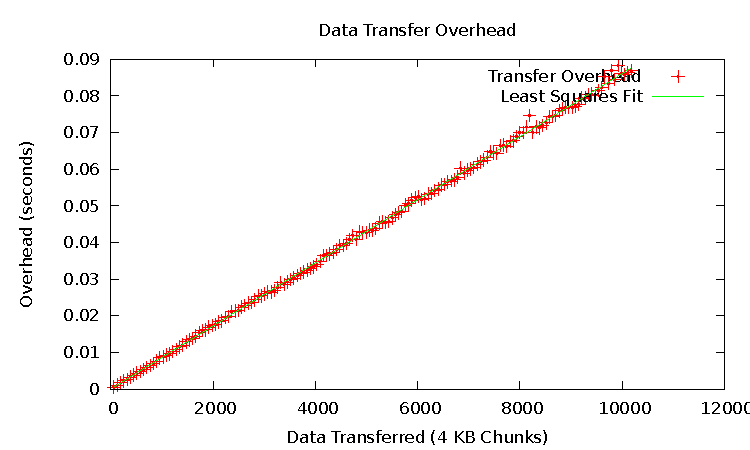
\includegraphics[scale=0.5, trim=40mm 0mm 20mm  0mm]{tachyon/dataData.pdf}
\caption{Data Transfer Overhead}
\label{tach:fig:dover}
\end{minipage}\begin{minipage}[b]{0.49\linewidth}
\centering
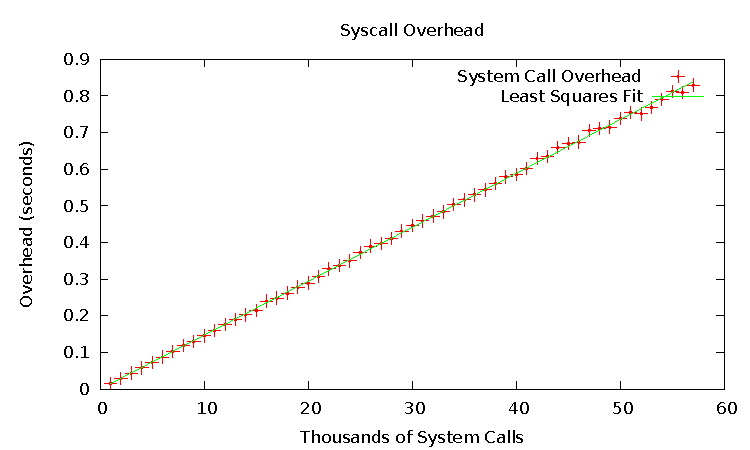
\includegraphics[scale=0.5]{tachyon/sysData.pdf}
\caption{Syscall Overhead}
\label{tach:fig:sover}
\end{minipage}
\end{figure*}

In Figure \ref{tach:fig:dover}, we see the overhead is in a linear relationship.
The overhead here is the total overhead
time for the system. While they make a difference for small data transfers, they are
rapidly dominated. This can be seen by the rapid transition to a tight grouping
around a linear relationship.


In Figure \ref{tach:fig:sover}, we again observe a nice linear relationship, showing no residual effects on performance from processing a system call. It shows that it takes less than a second of overhead to process 60,000 syscalls.

When varying the CPU load of the traced program, no noticeable difference in execution time was noticed, as we do not intercept regular computation, only system calls.

Given this, if it is known how many system calls are used, how much data is being
transferred, and how much time is being spent on the CPU, we can model how long
a given workload would take under our tracer.
\tachyon previously incurred a large number of copies and control transfers to move buffers around
in comparison with the register fetching it does for simple system calls, and
the remote memory fetch path is not optimized in the OS. However, a kernel patch
allowing for \texttt{mmap} to be used on the special file \texttt{/proc/pid/mem}
considerably ameliorate this, resulting in the new statistics above.

\paragraph{Tandem execution CPU time.}
The final source of overhead is in CPU operations.  Since \tachyon
sleeps when system calls are not being issued, it does not slow down
applications that are CPU-intensive. This is a significant advantage
over instruction-level interposition tools such as Pin~\cite{luk:2005} and
Valgrind~\cite{nethercote:2003:valgrind}, which typically suffer at least several
times overhead.

However, we are running both $\unpatched$ and $\patched$. We verified
that \tachyon can utilize independent cores to run both programs with
no additional overhead (other than the memory transfer and syscall
overhead measured above). Thus, we conclude that \tachyon can utilize
multi-core to test patches.

\paragraph{Efficiency on real programs.}

To test the efficiency of \tachyon interposition, we measured its
tandem execution against \texttt{strace} and \texttt{gdb}'s reverse
execution.  {\tt strace} is a tool built on top of \texttt{ptrace}
used to monitor system calls.  \texttt{gdb} allows programs to
back-step through operations.\footnote{We were unable to test against
  what is likely the most similar system, R2~\cite{guo:2008}, as it is
  both Windows only and requires build-time support (as well as not
  being public).} Note these tools have different goals than \tachyon;
we only use them to evaluate performance.

\texttt{gdb}'s replay mechanism derived from its reversible debugging
support. However, it proved wholly unsuitable for regions of more than
a few instructions. Due to a lack of SSE support, memcpy would be
improperly rewound and replayed. Additionally, even then the recording
overhead was more than 100x native execution, and built up a huge
memory data structure, making it impractical to benchmark.

\begin{figure}
\begin{small}
	\begin{center}
\begin{tabular}{|c|c|c|c|c|c|c|c|}
\hline
Program & Load & \tachyon  & \texttt{strace} \\
\hline \hline
\texttt{compress}  & 32M Random & 1.41  & 19.78 \\
\hline
\texttt{primegaps} & First 35 & 1.00 & 1.00 \\
\hline
\texttt{mencoder}  & h264 & 1.07 & 1.12\\
\hline
\end{tabular}
\end{center}
\end{small}
\caption{Tracing Performance (relative to native execution)}
\label{tach:fig:strace}
\end{figure}

The results compared to \texttt{strace} are shown in
Figure~\ref{tach:fig:strace}.  Overall, \tachyon was faster, sometimes by a
large margin, than a comparable syscall interposition scheme. 
This is partially because \tachyon can and does process some of its overhead while the traced program is doing work, but mostly due to the massively improved facility for retrieving remote memory via our patch to mmap /proc/pid/mem.

\paragraph{Web Server Tests.} We also tested the throughput of
\texttt{lighttpd} and \texttt{thttpd} when monitored under \tachyon.
In this test, we use ApacheBench (ab) configured to make 1000 requests
in two threads, downloading 4096 byte web page.  We ran the experiment
in two scenarios: on localhost and across the Internet.  

In the network experiment, the web servers ran at one university, and
requests were made from another university on the opposite US coast.
There was no detectable degradation for \texttt{thttpd}, and only
about a 30\% slowdown for \texttt{lighttpd}. Essentially, what this
shows is that while the system does not deal well with applications
whose progress is primarily based on the rate at which they can issue
system calls, when we move closer to a real deployment, applications
do not tend to have that as their primary limiting factor.

In the second experiment, we ran ab on localhost.  This is a
worst-case test because both web servers spin in a tight loop on a
syscall (\texttt{lighttpd} spins on \texttt{epoll}, and
\texttt{thttpd} on \texttt{poll}). 
This creates a pathological case for \tachyon, because the application
spends most of its time neither doing IO, nor doing computation, but
instead spends most of its time moving across the system call barrier.

\tachyon
took 8.9 times longer on $\texttt{lighttpd}$ (throughput decreased to
10\% of original values) and 14.2 times longer on $\texttt{thttpd}$
(throughput decreased to 7\% of original values).

To round things out, we also ran a test over a few hops on the local network.
As expected, intermediate results were measured to be between the two, with
1.17 times untraced completion to complete the test with $\texttt{thttpd}$, and 3.72
times untraced completion to complete the test with $\texttt{lighttpd}$.

With a more real network (or a more complicated webapp), we can see the
slowdown is lessened. With a real network, \texttt{epoll} will spend more
time waiting, diminishing the perceived effects.

% \texttt{mencoder} was run in a record only mode, as
% it aggressively uses all available cores, and so attempting to run two copies in
% tandem (which none of the other tracing utilities do) will necessarily produce
% massive overhead, and not truly measure the overhead of \tachyon.



%%% Local Variables: 
%%% mode: latex
%%% TeX-master: "paper"
%%% End: 

\section{Discussion}
\label{tach:sec:discussion}

\paragraph{Other Patch Testing Scenarios.} While throughout this chapter we have focused on online patch testing
where the patched version is run live, we could also run the unpatched
version live.  We note that the live program can continue executing
after a deviation, but currently the syscall sync application cannot.
Thus, by running the patched live, we are assuming that after a
deviation the right thing is to continue executing the patched
version.  However, by running the  unpatched version live, we can
check for incompatibilities while allowing for the original program to
continue executing after a deviation.

\paragraph{Honeypots.} \tachyon can also be used as a type of
lightweight honeypot. Let $\patched$ be a patch for a security
vulnerability, and $\unpatched$ be the vulnerable program. Observe
that $\patched$ and $\unpatched$ differ on exploits by definition.  By
running $\patched$ and $\unpatched$ in-tandem, \tachyon will report a
deviation on attacks.

A clever approach to running a honeypot is to run $\patched$ as the live
program, with $\unpatched$ as the sync. In this setting an attacker
only seeing the buggy program. \tachyon will report attacks, e.g., by
logging a deviation when shellcode tries to execute \texttt{/bin/sh}.
However, the system is safe from a real compromise because \tachyon
can be configured to abort execution after the deviation.



\paragraph{Debugging.} One of the most difficult to debug classes of
bugs is commonly known as heisenbugs. These are bugs which will
seemingly randomly occur or not occur with all of the inputs the
programmer knows about held constant. These traces, and the
associated replay mechanism, provide a way to step through the program
in a completely deterministic way, so that once a heisenbug has been
caught with tracing on, it has been captured and the sequence leading
to it can be carefully explored and debugged. As we capture all
inputs, this also makes it possible for the programmer to debug a
crash that took place on another machine, without having to try to
replicate the OS state to reproduce the crash.

\paragraph{Efficiency.}
Recall \tachyon uses user-land syscall interposition, and has
our approach to syscall interposition as its primary source of overhead
Currently, interposing on each system call on the live program requires 4
context switches. \tachyon context switches from $\patched$ to the
kernel, from the kernel to \tachyon, from \tachyon back to the kernel,
and finally back to $\patched$. Normal operation only has two context
switches: from user to kernel space, and back again.  A kernel-space
interposition scheme would also have only two switches. 

Recall from \S~\ref{tach:sec:eval} the overhead from copying data is almost
linear in the amount data transferred between $\patched$ and
$\unpatched$. A basic in-kernel approach would still have a linear
overhead (since data has to be copied into both virtual memory
spaces), but likely with a smaller constant factor.

Our user-land approach was chosen because it offers a clean separation
of functionality, isn't kernel dependent, and offers an easier
development environment.  Moving the system call interposition into
the kernel would not have these advantages, but would likely improve
performance. We leave further study of in-kernel tandem execution schemes
as future work.

%%% Local Variables: 
%%% mode: latex
%%% TeX-master: "paper"
%%% End: 


%Related Work
\section{Related Work}
\label{sec:related}
%  Starting blurb similar to backround blurb, surprised by this...
As this work stands at the confluence of compilation, instruction set architectures, static analysis, and type theory, there is a great deal of prior work that provided the foundation to create \bitr. There have been other attempts to perform binary type recovery. Type theorists have explored the relevant formal systems that enable us to appropriately describe the constraints imposed by the wide variety of instructions. Others have tried to build decompilers, each of which contains at least an attempt at type reconstruction.
%  Chunk related work into blobs and describe, reference to sections as you do it
\subsection{Types in Compiled Code}
In large part, previous work has considered dynamic approaches, which use execution traces to get information about concrete values. Another school of thought takes a more forensics-oriented approach, attacking the problem by looking for known data structures within a dump or trace. Finally, there is the school to which this work belongs, static type recovery, where the approach regenerates type information from a representation of the code, rather than from sample runs or matching known data structures.

\noindent {\bf Dynamic Type Description.}
Rewards~\cite{rewards} takes a dynamic, trace-oriented approach to the problem, taking execution traces and known system calls, and propagating types from system calls through the trace's reads and writes. The dynamic approach has the advantage that the analysis can know what values a memory location or register actually held at a given program point. Additionally, the dynamic approach does not have to solve the problem of indirect jumps, as when working with traces the next instruction is precisely computed. Finally, since Rewards had exact aliasing information via pointer values on each trace, flowing information from the system call barrier (their major outside source of types) is easier. While Rewards seems limited for types not present during the crossing of the system call barrier, its dynamic approach, and information from the crossing of the system call barrier could provide additional constraints to a system like \bitr\ to further improve accuracy. Howard~\cite{Slowinska2011} extends the work of Rewards by focusing on access patterns instead of simple propagation, and annotating variables from the original code, rather than locations on a dump.

\noindent {\bf Type Forensics.}
Another approach known as shape analysis~\cite{August, Haller2013a,White2013,Jung2009,Cozzie} uses dynamic traces to generate shape graphs, which they then analyze to make guesses at the types of memory locations. The systems generate the shape graph by first generating a trace, then matching the access pattern to the simplest possible graph of type structures. Some generate this trace from the compiled program, and some must annotate the program prior to compilation to achieve this trace. Once the system generates the shape graph, it compares the shape graph to multiple possibilities of what the data structure might be in attempt to classify it e.g. as a binary tree or linked list. One benefit of this technique is that when the system finds a match, more information on a name of the data structure may be available. However, if the program uses a data structure not expected by the system, some of these methods will fall short. For example, MemPick will report it to be a generic graph. It also suffers from the standard dynamic analysis issue of being unable to generate types for paths the test cases did not drive it down.

\noindent {\bf Static Type Recovery.}
Like TIE~\cite{tie}, we built \bitr\ on BAP~\cite{bap}, and also took the approach of trying to generate ranges of constraints. However, TIE performs much worse under our metric, which we feel more fully represents accuracy of more complicated types. TIE's metric is problematic for the reasons described in~\cite{sw}, but the proposed replacement metric is still dependent on a notion of distance. TIE is also slow, which hobbles its use as a large scale analysis tool. The use of DIVINE's methods was one of the bottlenecks, which we avoided in \bitr\ by recovering the type of everything that is addressable through the registers or a constant integer used along a dataflow that ended in a read or write. While the type system of TIE included structure types, TIE would rarely infer them, though its metric did not demonstrate this. Finally, if run on a static binary (e.g. without dynamic library hints), the amount TIE could infer itself was minimal.

SecondWrite~\cite{sw} instead takes the approach of lifting to a LLVM-based IR~\cite{llvm}, then using \texttt{mem2reg} to detect variables and LLVM pointer analysis to compute the types. Their reconstruction is simpler and faster than TIE's, but the approach has issues: \texttt{mem2reg} is a nice shortcut, but has the problem that \texttt{mem2reg} will not promote anything which has a use other than a load or store~\cite{llvm}. As a result, if on-stack references are in use, those stack slots will not be properly promoted to variables. Additionally, dependence on pointer analysis leaves them without a way to detect recursive types within their framework, and makes nested structures unlikely to work.

Another work focusing primarily on structure recovery~\cite{comprecon} approached the problem from the angle of figuring out what idioms compilers used to address arrays and structs, and then tried to reconstruct structs and arrays. However, by the authors' own admission, this approach cannot handle nested structs. Additionally, their dependence on assumptions about how the compiler will act and how the source language must work cause the output to be of limited use for understanding properties of code which was not necessarily built by the compilers or language expected.

\subsection{Type Theory}
Some of the inspiration for this form of type characterization \S\ref{sec:typesys} came from intersection typing~\cite{Jim1995,Shao1993}. Though we did not end up using intersection types for inferrability purposes (even the decidability of the inference turns out to be difficult and limited~\cite{interdecide}), this work informed our choice of a constraint-intersection \S\ref{sec:infmeth} approach instead of type-intersection approach.

Earlier efforts to generate typed assembly~\cite{tal,stal} also bear similarity to our work. Typed assembly language methodologies are attempting to assign types to the registers in compiled code during compilation. Some of the TAL ideas are applicable, and still others could potentially help in future reconstruction work as safer types.
However, the majority are inappropriate for the work because the compiler or author must make the code conform to the system, rather than the system describing the code.

\subsection{Decompilation}
One of the main applications for type reconstruction is decompilation. Some approaches~\cite{tydecomp} even suggest that the type reconstruction can help guide the decompilation itself rather than simply being a set of annotations applied at the end. This idea has existed~\cite{dolgova2009automatic} in decompilation for a while, but progress has been slow. More recent decompilers~\cite{phoenix} have used some of the other research~\cite{tie} in the area to improve their results as well. Given the poor state of affairs in Hex-Rays~\cite{ida}, more work in this field could improving the usability of much of the decompiler work would not be surprising.


%Conclusion
\section{Conclusion}
\label{sec:conclusion}
%  First something or other (narrow until you've got it)
\bitr\ forms the first type recovery system able to recover \emph{recursive}, \emph{polymorphic}, and \emph{structure} types from compiled code.
%  Real Problem
Type reconstruction is a real problem encountered in a variety of areas, ranging from debugging of foreign code to decompilation and analysis.
%  We made a tool to deal with it
In this paper, we have shown that \bitr\ recovers types in a fashion which is both more accurate and specific than previous work. \bitr\ accomplishes this by applying techniques inspired by the field of programming languages. Finally, by being a general type system, \bitr\ forms a way of looking at type recovery that is more extensible and applicable to a wider variety of problems.

%Code is freely available at blah
%Well, it's not, so this point is absent


\backmatter
\singlespacing
\renewcommand{\bibsection}{\chapter{\bibname}}
\bibliographystyle{plain}
\bibliography{thesis,bitr/BiTR-0,tachyon/tachyon}

\end{document}
